% octopus-manual.tex -- the Octopus reference manual. Build with ./build.sh (or make).
\documentclass[11pt,a4paper,twoside,openany]{book}
% preamble.tex -- packages, fonts, colours, boxes and macros for the Octopus manual.
\usepackage[T1]{fontenc}
\usepackage[utf8]{inputenc}
\usepackage{plex-serif}            % body: IBM Plex Serif
\usepackage{plex-sans}             % headings, captions: IBM Plex Sans
\usepackage{plex-mono}             % code: IBM Plex Mono (matches the figures)
\usepackage{microtype}
\usepackage[a4paper,margin=2.2cm,headheight=14pt]{geometry}
\usepackage{graphicx}
\graphicspath{{figures/pdf/}{figures/paper/}{figures/png/}}
\usepackage{xcolor}
\usepackage{booktabs,longtable,array,tabularx,multirow,rotating,pdflscape,adjustbox}
\usepackage{caption,subcaption}
\newcolumntype{Y}{>{\raggedright\arraybackslash}X}   % a left-aligned X column (no justification gaps)
\usepackage{enumitem}
\usepackage{listings}
\usepackage{tikz}
\usetikzlibrary{arrows.meta,positioning,calc,shapes.geometric,fit,backgrounds,chains,decorations.pathreplacing,matrix}
\usepackage{pgf-umlsd}
\usepackage[most]{tcolorbox}
\usepackage{fancyhdr}
\usepackage{titlesec}
\usepackage{imakeidx}
\usepackage{amsmath,amssymb,pifont}
\usepackage[style=ieee,backend=biber,maxbibnames=6]{biblatex}
\addbibresource{references.bib}
\usepackage[hidelinks,pdfusetitle]{hyperref}
\usepackage[capitalise,noabbrev]{cleveref}

% ---- the palette of the SVG figure series, so TikZ figures match ----
\definecolor{octink}{HTML}{14212A}
\definecolor{octquiet}{HTML}{5E6E76}
\definecolor{octteal}{HTML}{0E7C73}
\definecolor{octamber}{HTML}{B45309}
\definecolor{octpurple}{HTML}{4B32A8}
\definecolor{octred}{HTML}{BE3F24}
\definecolor{octpaper}{HTML}{FCFBF8}
\definecolor{octmem}{HTML}{EAF1F6}
\definecolor{octio}{HTML}{F4F1FB}
\definecolor{octctl}{HTML}{FDF6E6}
\definecolor{octrule}{HTML}{5A6B75}

\makeindex[name=cfg,title=Index of configuration keys,columns=2]
\makeindex[name=idx,title=Index,columns=2]

% ---- typography ----
\titleformat{\chapter}[display]{\sffamily\bfseries\Huge\color{octink}}{\sffamily\mdseries\Large\color{octquiet}Chapter \thechapter}{0.6em}{}
\titleformat*{\section}{\sffamily\bfseries\Large\color{octink}}
\titleformat*{\subsection}{\sffamily\bfseries\large\color{octink}}
\titleformat*{\subsubsection}{\sffamily\bfseries\color{octink}}
\captionsetup{font={sf,small},labelfont={bf,color=octink},labelsep=period,width=0.92\textwidth}
\setlist{nosep,leftmargin=1.4em}
\pagestyle{fancy}\fancyhf{}
\fancyhead[LE]{\sffamily\small\nouppercase\leftmark}\fancyhead[RO]{\sffamily\small\nouppercase\rightmark}
\fancyfoot[C]{\sffamily\small\thepage}
\renewcommand{\headrulewidth}{0.3pt}
\setlength{\parskip}{0.35em}\setlength{\parindent}{0pt}
\setcounter{secnumdepth}{2}\setcounter{tocdepth}{1}

% ---- code ----
\lstset{basicstyle=\ttfamily\small,backgroundcolor=\color{octpaper},frame=single,rulecolor=\color{octrule!40},
  framesep=4pt,xleftmargin=4pt,breaklines=true,breakatwhitespace=false,columns=fullflexible,keepspaces=true,
  showstringspaces=false,commentstyle=\color{octquiet},keywordstyle=\color{octpurple}\bfseries,stringstyle=\color{octteal},
  upquote=true,literate={→}{{$\rightarrow$}}1 {←}{{$\leftarrow$}}1 {—}{{---}}1 {–}{{--}}1 {·}{{$\cdot$}}1 {≈}{{$\approx$}}1 {≠}{{$\neq$}}1 {×}{{$\times$}}1}
\lstdefinestyle{shell}{language=bash,morekeywords={cmake,make,git,python,bash,cd,export},keywordstyle=\color{octink}\bfseries,commentstyle=\color{octquiet}\itshape}
\lstdefinestyle{csv}{language={},commentstyle=\color{octquiet},morecomment=[l]{\#}}
\lstdefinestyle{cpp}{language=C++,morekeywords={override,virtual,uint64_t,uint16_t,uint8_t,size_t,Message,ControllerAction}}
\lstdefinestyle{plain}{language={}}

% ---- boxes ----
\newtcolorbox{wherebox}[1][Where in the code]{enhanced,colback=octmem!60,colframe=octrule,fonttitle=\sffamily\bfseries,title={#1},before upper=\raggedright,arc=2pt,boxrule=0.6pt,left=5pt,right=5pt,top=4pt,bottom=4pt,before skip=8pt,after skip=10pt}
\newtcolorbox{trapbox}[1][Trap]{enhanced,colback=octctl,colframe=octamber,fonttitle=\sffamily\bfseries,title={#1},before upper=\raggedright,arc=2pt,boxrule=0.6pt,left=5pt,right=5pt,top=4pt,bottom=4pt,before skip=8pt,after skip=10pt}
\newtcolorbox{notebox}[1][Design note]{enhanced,colback=octio,colframe=octpurple,fonttitle=\sffamily\bfseries,title={#1},before upper=\raggedright,arc=2pt,boxrule=0.6pt,left=5pt,right=5pt,top=4pt,bottom=4pt,before skip=8pt,after skip=10pt}
\newtcolorbox{findbox}{enhanced,colback=octpaper,colframe=octrule!50,arc=2pt,boxrule=0.5pt,left=5pt,right=5pt,top=3pt,bottom=3pt,before skip=6pt,after skip=8pt,fontupper=\small,before upper=\raggedright}

% ---- macros ----
\newcommand{\octopus}{Octopus}
\newcommand{\brkus}{\textunderscore\allowbreak}
\newcommand{\code}[1]{{\let\_\brkus\ttfamily #1}}   % monospace that may break after an underscore
\newcommand{\file}[1]{\path{#1}}   % verbatim argument: write raw _ and *, breaks at / and _
\newcommand{\key}[1]{\code{#1}\index[cfg]{#1@\code{#1}}}
\newcommand{\env}[1]{\code{#1}\index[idx]{#1@\code{#1} (environment)}}
\newcommand{\state}[1]{\textsf{#1}}
\newcommand{\act}[1]{\code{#1}\index[idx]{#1@\code{#1} (FSM action)}}
\newcommand{\evt}[1]{\code{#1}}
\newcommand{\stamp}[1]{\code{#1}}
\newcommand{\col}[1]{\textsf{#1}}
\newcommand{\figwide}[3]{\begin{figure}[htbp]\centering\includegraphics[width=\textwidth]{#1}\caption{#2}\label{#3}\end{figure}}
\newcommand{\figmed}[4]{\begin{figure}[htbp]\centering\includegraphics[width=#4\textwidth]{#1}\caption{#2}\label{#3}\end{figure}}
\newcommand{\gitcommit}{3cb0f8b0\unskip}
\newcommand{\whatyoufind}[1]{\begin{findbox}\textbf{\sffamily What you will find here.} #1\end{findbox}}


\title{Octopus\\[0.3em]\large A cycle-accurate memory-system simulator for predictable multicores\\[0.6em]\normalsize Reference manual}
\author{Fanos Research Lab, McMaster University}
\date{Revision \gitcommit\ \textperiodcentered\ \today}

\begin{document}
\frontmatter
\begin{titlepage}
  \centering
  \vspace*{2.5cm}
  
\includegraphics[width=4.2cm]{logo.png}\par\vspace{1.4cm}
  {\sffamily\bfseries\fontsize{40}{44}\selectfont\color{octink}Octopus\par}\vspace{0.5cm}
  {\sffamily\Large\color{octquiet}A cycle-accurate memory-system simulator\\for predictable multicores\par}\vspace{1.2cm}
  {\sffamily\LARGE\color{octink}Reference manual\par}\vspace{2.5cm}
  {\sffamily\large Fanos Research Lab \textperiodcentered\ McMaster University\par}\vspace{0.4cm}
  {\sffamily\color{octquiet}Revision \gitcommit\ \textperiodcentered\ \today\par}
  \vfill
  {\sffamily\small\color{octquiet}\url{https://github.com/FanosResearch/OctopusSimulator}\par}
\end{titlepage}

\chapter*{About this manual}
\addcontentsline{toc}{chapter}{About this manual}

To be written: what Octopus is, who this manual is for, how to read it, where the sources live.

\tableofcontents
\listoffigures

\mainmatter
\chapter{Introduction}\label{ch:introduction}

\whatyoufind{To be written.}

\chapter{Getting started}\label{ch:getting-started}

\whatyoufind{To be written.}

\chapter{System organization}\label{ch:system-organization}

\whatyoufind{The four principles the simulator is built on and the two base classes that
carry them; the clock model, which is the reason every latency it reports is comparable; the
map of components and the classes behind them; and the exact system that
\file{MultiCoreSystem.csv} builds when you run the shipped configuration --- the system every
later chapter's figures are drawn on.}

\section{Design principles}

Octopus models a multicore memory hierarchy as a \emph{network of clocked, configurable
components} joined by bounded, back-pressured \emph{interfaces}. A memory request is a
first-class \code{Message} object that travels this network; a single global clock steps every
component; and every hop is timestamped for the Logger. Four principles shape the code, and
they are realised through two base classes that every component inherits
(\cref{tab:base-classes}).

\begin{itemize}
\item \textbf{Modularity.} Each component is self-contained behind a narrow interface, so
  changing one does not ripple into others. A cache controller does not know whether it is an
  L1 or the LLC, nor which protocol it runs; a bus does not know what it carries.
\item \textbf{Extensibility.} Inheritance and polymorphism: a new arbiter, replacement policy,
  topology or memory model is a subclass with a handful of virtual methods; a new coherence
  protocol is a CSV file. The effect shows in the code size of protocols derived from a common
  family (\cref{ch:coherence-engine}).
\item \textbf{Configurability.} Every component derives from \code{Configurable}: it reads its
  defaults from its own CSV, a parent may override a child's, and the command line overrides
  everything, so the whole design space is reachable without recompiling
  (\cref{ch:configuration}).
\item \textbf{Integrability.} The two endpoints --- the request source and the memory sink ---
  are swappable for external simulators: a trace-driven CPU or gem5 on one side, a fixed-latency
  model or MCsim's DDR controllers on the other, with the hierarchy between them unchanged
  (\cref{ch:integration-modes}).
\end{itemize}

\begin{table}[htbp]\centering\small
\caption{The two base classes every component inherits.}\label{tab:base-classes}
\begin{tabularx}{\textwidth}{@{}lX@{}}
\toprule base class & gives every component \\ \midrule
\code{ClockedObj} & \code{m\_clk\_period} and \code{cycleProcess()}: the component can be advanced one tick by the \code{ClockManager} \\
\code{Configurable} & \code{name}, \code{parent\_name}, \code{parameters}, \code{parseFile()}: hierarchical parameters read from CSV and overridable from the CLI \\
\bottomrule
\end{tabularx}
\end{table}

\section{The clock model}

\begin{figure}[htbp]\centering
% The clock model: one ClockManager advances every ClockedObj by one tick; components
% never call each other, they only exchange Messages through interfaces between ticks.
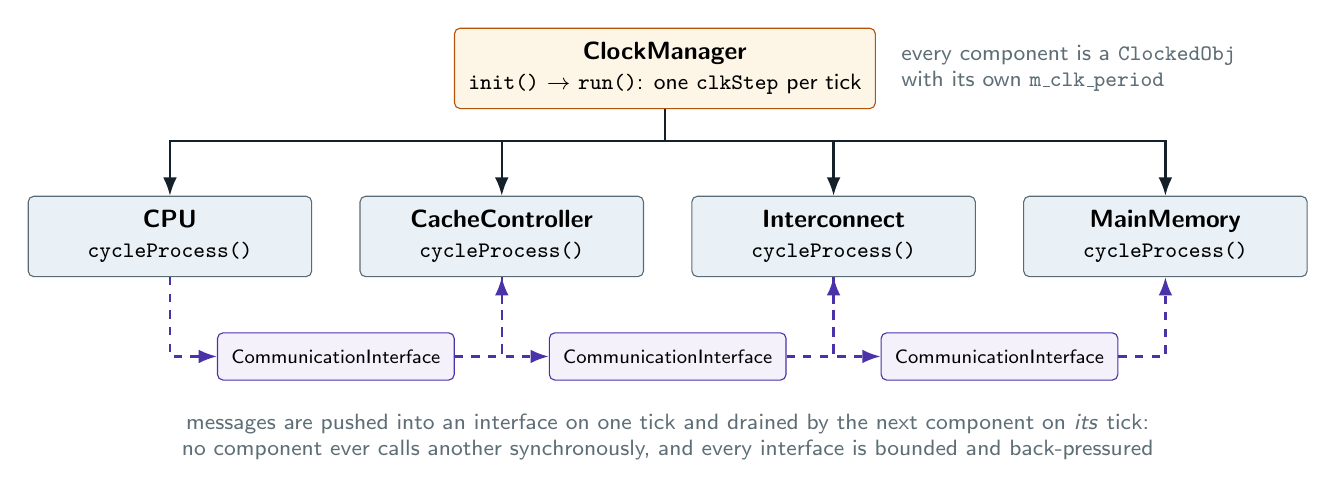
\begin{tikzpicture}[
  font=\sffamily\small, >=Latex,
  box/.style={draw=octrule, fill=white, rounded corners=2pt, minimum height=9mm, inner sep=5pt, align=center},
  clk/.style={box, fill=octctl, draw=octamber, minimum width=34mm},
  comp/.style={box, fill=octmem, draw=octrule, minimum width=36mm},
  iface/.style={box, fill=octio, draw=octpurple, minimum width=22mm, minimum height=6mm, font=\sffamily\scriptsize},
  wire/.style={->, thick, octink},
  msg/.style={->, thick, octpurple, dashed},
]
  \node[clk] (cm) {\textbf{ClockManager}\\\footnotesize \code{init()} $\rightarrow$ \code{run()}: one \code{clkStep} per tick};
  \node[comp, below left=11mm and 18mm of cm] (cpu) {\textbf{CPU}\\\footnotesize \code{cycleProcess()}};
  \node[comp, right=6mm of cpu] (l1) {\textbf{CacheController}\\\footnotesize \code{cycleProcess()}};
  \node[comp, right=6mm of l1] (ic) {\textbf{Interconnect}\\\footnotesize \code{cycleProcess()}};
  \node[comp, right=6mm of ic] (mem) {\textbf{MainMemory}\\\footnotesize \code{cycleProcess()}};
  \foreach \c in {cpu,l1,ic,mem} \draw[wire] (cm.south) -- ++(0,-4mm) -| (\c.north);
  \node[iface, below=7mm of $(cpu.south)!0.5!(l1.south)$] (i1) {CommunicationInterface};
  \node[iface, below=7mm of $(l1.south)!0.5!(ic.south)$] (i2) {CommunicationInterface};
  \node[iface, below=7mm of $(ic.south)!0.5!(mem.south)$] (i3) {CommunicationInterface};
  \draw[msg] (cpu.south) |- (i1.west);  \draw[msg] (i1.east) -| (l1.south);
  \draw[msg] (l1.south) |- (i2.west);   \draw[msg] (i2.east) -| (ic.south);
  \draw[msg] (ic.south) |- (i3.west);   \draw[msg] (i3.east) -| (mem.south);
  \node[below=3mm of i2, font=\sffamily\footnotesize, text=octquiet, align=center] {messages are pushed into an interface on one tick and drained by the next component on \emph{its} tick:\\no component ever calls another synchronously, and every interface is bounded and back-pressured};
  \node[right=2mm of cm, font=\sffamily\footnotesize, text=octquiet, align=left] {every component is a \code{ClockedObj}\\with its own \code{m\_clk\_period}};
\end{tikzpicture}

\caption{The clock model. One \code{ClockManager} advances every \code{ClockedObj} by one tick;
components exchange messages only through interfaces, which the next component drains on its
own tick.}
\label{fig:clock-loop}
\end{figure}

The \code{ClockManager} owns the simulation loop. On each \code{clkStep} it advances every
\code{ClockedObj} whose period has elapsed by calling its \code{cycleProcess()}
(\cref{fig:clock-loop}). Components never call each other synchronously: they communicate only by
placing \code{Message}s into interfaces, which the receiving component drains when it is next
stepped. That decoupling is what makes the hierarchy modular and back-pressured --- an interface
that is full simply refuses the push, and the sender tries again on its next tick.

Because all components step under one manager, latencies are consistent system-wide: the Logger
measures every stage of a request in the \emph{originating core's} clock, whichever component
stamps it (\cref{ch:monitoring}). Each component carries its own \code{m\_clk\_period}, so a
memory model may legitimately tick at a different rate from the cores; in the shipped
configuration every period is 100 and one tick is one cycle everywhere.

\begin{notebox}[Design note: a clock-period bug worth knowing about]
The MCsim bridge once ticked the DRAM model once per \emph{manager} step rather than once per
LLC cycle --- a hundred DRAM cycles per core cycle --- so DRAM looked like a one-cycle device.
The LLC's period is now passed into the bridge; any DRAM number produced before that fix is
untrustworthy. The lesson generalises: a component with its own period must be stepped by the
manager, never by whoever happens to call it.
\end{notebox}

\section{Component map}

\figmed{SystemConfiguration3.pdf}{What a configured system can contain: clusters of cores with
private caches on direct interconnects, further cache levels inside or across clusters, a
shared last-level cache and main memory --- all of it chosen by configuration, not
hard-coded.}{fig:organization}{0.62}

A system is clusters of CPU cores, each with private caches and a direct interconnect, joined
through configurable interconnects to a shared LLC and main memory (\cref{fig:organization}).
\Cref{tab:roles} names the class behind each role; \cref{fig:classes} shows how they relate.

\begin{table}[htbp]\centering\small
\caption{Roles and the classes that play them.}\label{tab:roles}
\begin{tabularx}{\textwidth}{@{}lp{0.47\textwidth}X@{}}
\toprule role & class(es) & notes \\ \midrule
clock & \code{ClockManager}, \code{ClockedObj} & drives \code{cycleProcess()} each tick \\
configuration & \code{Configurable} & hierarchical CSV + CLI parameters \\
core & \code{CPU} (trace), \code{ExternalCPU} (gem5) & issues \code{Message}s; the trace CPU has an out-of-order window of \key{m\_number\_of\_OoO\_requests} \\
transport & \code{CommunicationInterface} & \code{pushMessage} / \code{peekMessage} / \code{popFrontMessage}; bounded \\
message & \code{Message} & \code{msg\_id}, \code{addr}, \code{cycle}, \code{owner}, \code{source}, \code{data}, \code{kind} \\
cache & \code{BaseController} $\rightarrow$ \code{CacheController} $\rightarrow$ \code{CacheControllerExclusive}, \code{CacheController\_End2End}, \code{CacheControllerDirectory} & processing queue + handlers (\cref{ch:cache-controller}) \\
coherence & \code{CoherenceProtocolHandler} $\rightarrow$ MSI / MESI / MOESI, their LLC and directory variants & driven by \code{FSMReader} (\cref{ch:coherence-engine}) \\
data & \code{CacheDataHandler} $\rightarrow$ \code{CacheDataHandler\_COTS} & array, MSHRs, write-back buffer, replacement, port arbiter \\
interconnect & \code{InterconnectTopology} + \code{InterconnectController} + \code{Arbiter} & bus, mesh, NoC (\cref{ch:interconnects}) \\
memory & \code{MainMemoryController} (fixed latency), \code{MCsimInterface} & the sink (\cref{ch:main-memory}) \\
monitoring & \code{Logger}, \code{DebugPrint} & \cref{ch:monitoring} \\
\bottomrule
\end{tabularx}
\end{table}

\figwide{Octopus.pdf}{The class diagram. Cache-related classes in red, interconnect-related in
blue, utilities in white.}{fig:classes}

\section{The system as shipped}\label{sec:shipped-system}

\begin{figure}[htbp]\centering
% The system MultiCoreSystem.csv builds: four cores with private L1s on a TripleBus, one
% shared inclusive LLC, a point-to-point memory bus and a fixed-latency main memory.
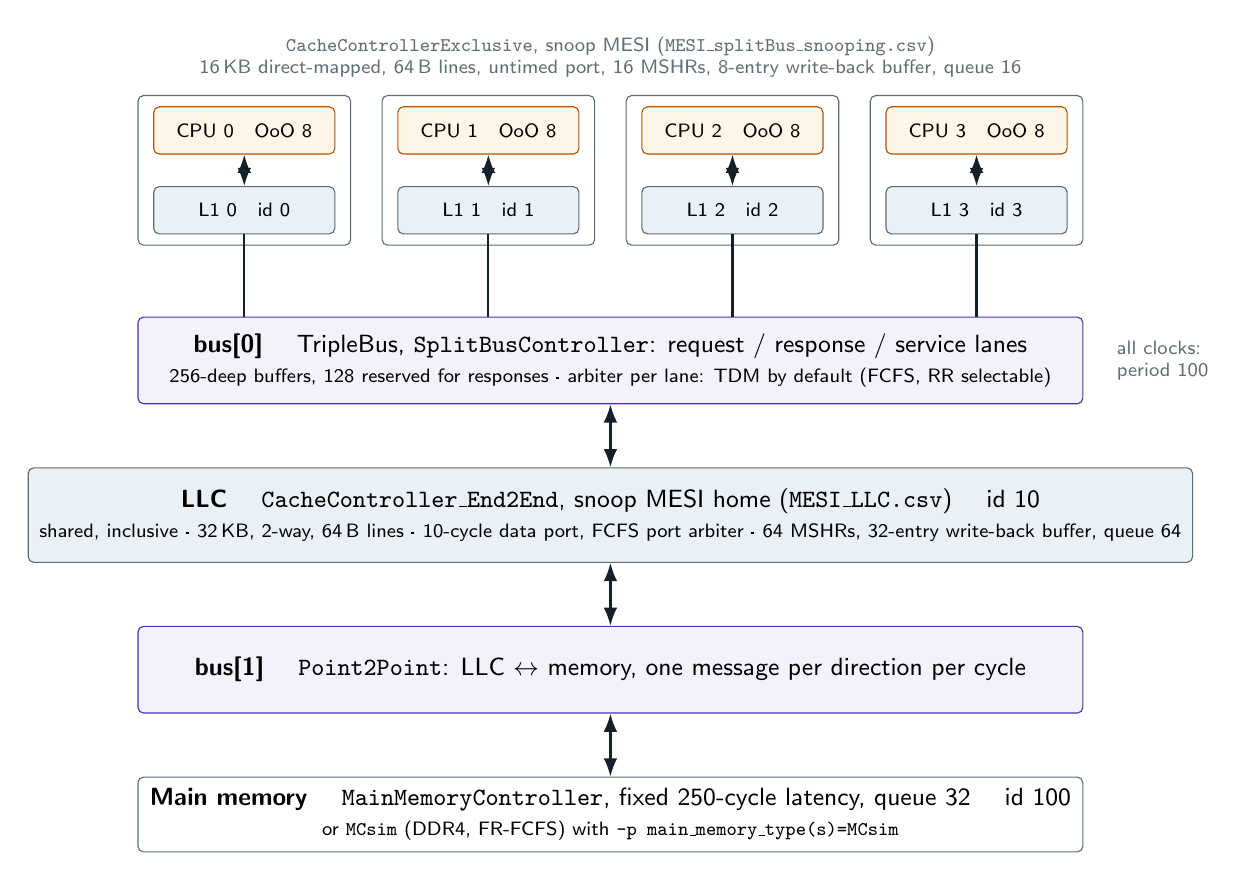
\begin{tikzpicture}[
  font=\sffamily\small, >=Latex,
  box/.style={draw=octrule, rounded corners=2pt, inner sep=4pt, align=center, minimum height=8mm},
  core/.style={box, fill=white, minimum width=27mm, minimum height=19mm},
  cpu/.style={box, fill=octctl, draw=octamber, minimum width=23mm, minimum height=6mm, font=\sffamily\scriptsize},
  l1/.style={box, fill=octmem, minimum width=23mm, minimum height=6mm, font=\sffamily\scriptsize},
  bus/.style={box, fill=octio, draw=octpurple, minimum height=11mm},
  llc/.style={box, fill=octmem, draw=octrule, minimum height=12mm},
  mem/.style={box, fill=white, minimum height=9mm},
  sidenote/.style={font=\sffamily\scriptsize, text=octquiet},
  wire/.style={thick, octink},
]
  \foreach \k in {0,1,2,3} {
    \node[core] (c\k) at (\k*31mm, 0) {};
    \node[cpu] (cpu\k) at ($(c\k.north)+(0,-4.5mm)$) {CPU \k \quad OoO 8};
    \node[l1] (l1\k) at ($(c\k.south)+(0,4.5mm)$) {L1 \k \quad id \k};
    \draw[wire, <->] (cpu\k) -- (l1\k);
  }
  \node[font=\sffamily\scriptsize, text=octquiet, align=center, above=1mm of $(c1.north)!0.5!(c2.north)$]
    {\code{CacheControllerExclusive}, snoop MESI (\code{MESI\_splitBus\_snooping.csv}) \\ 16\,KB direct-mapped, 64\,B lines, untimed port, 16 MSHRs, 8-entry write-back buffer, queue 16};
  \node[bus, below=9mm of $(c1.south)!0.5!(c2.south)$, minimum width=120mm] (b0)
    {\textbf{bus[0]} \quad TripleBus, \code{SplitBusController}: request / response / service lanes \\ \scriptsize 256-deep buffers, 128 reserved for responses \textperiodcentered\ arbiter per lane: TDM by default (FCFS, RR selectable)};
  \foreach \k in {0,1,2,3} \draw[wire] (l1\k.south) -- (l1\k.south |- b0.north);
  \node[llc, below=8mm of b0, minimum width=120mm] (llc)
    {\textbf{LLC} \quad \code{CacheController\_End2End}, snoop MESI home (\code{MESI\_LLC.csv}) \quad id 10 \\ \scriptsize shared, inclusive \textperiodcentered\ 32\,KB, 2-way, 64\,B lines \textperiodcentered\ 10-cycle data port, FCFS port arbiter \textperiodcentered\ 64 MSHRs, 32-entry write-back buffer, queue 64};
  \draw[wire, <->] (b0.south) -- (llc.north);
  \node[bus, below=8mm of llc, minimum width=120mm] (b1)
    {\textbf{bus[1]} \quad \code{Point2Point}: LLC $\leftrightarrow$ memory, one message per direction per cycle};
  \draw[wire, <->] (llc.south) -- (b1.north);
  \node[mem, below=8mm of b1, minimum width=120mm] (mem)
    {\textbf{Main memory} \quad \code{MainMemoryController}, fixed 250-cycle latency, queue 32 \quad id 100 \\ \scriptsize or \code{MCsim} (DDR4, FR-FCFS) with \code{-p main\_memory\_type(s)=MCsim}};
  \draw[wire, <->] (b1.south) -- (mem.north);
  \node[sidenote, right=3mm of b0.east, align=left] {all clocks:\\period 100};
\end{tikzpicture}

\caption{The system \code{MultiCoreSystem.csv} builds. Four trace-driven cores with private
MESI L1s on a TripleBus, one shared inclusive LLC, a point-to-point memory bus and a
fixed-latency main memory. Every number is a configuration key (\cref{app:config-keys}).}
\label{fig:shipped-system}
\end{figure}

Running \code{Octopus\_Simulator -s MultiCoreSystem} instantiates the C++ system class
\code{MultiCoreSystem} and configures it from
\file{configuration/SystemConfigurations/MultiCoreSystem.csv}. \Cref{fig:shipped-system} is that
system; it is the one every route, datapath and sequence figure in this manual is drawn on, and
the one the tutorial runs first. The points that matter when reading a report:

\begin{itemize}
\item \textbf{Four cores} (\key{num\_cores}), each a trace-driven \code{CPU} with an
  out-of-order window of eight outstanding requests, and each with a private L1 of
  \code{CacheControllerExclusive} running snoop MESI --- 16\,KB, direct-mapped, 64-byte lines,
  an untimed data port, 16 MSHRs, an 8-entry write-back buffer and a 16-deep processing queue.
\item \textbf{\code{bus[0]}} is a TripleBus under a \code{SplitBusController}: three lanes ---
  request, response, service --- each with its own arbiter, TDM by default
  (\file{SplitBusController.csv}); 256-deep buffers with 128 entries reserved for in-flight
  responses so that the request lane stalls before responses can overflow.
\item \textbf{The LLC} (id 10) is a \code{CacheController\_End2End}: shared, inclusive, 32\,KB,
  2-way, 64-byte lines, a 10-cycle data port with an FCFS port arbiter, 64 MSHRs, a 32-entry
  write-back buffer and a 64-deep queue. Its \code{MESI\_LLC} FSM is the home of the protocol.
\item \textbf{\code{bus[1]}} is point-to-point between the LLC and memory (id 100).
\item \textbf{Main memory} is a \code{MainMemoryController} with a fixed 250-cycle latency;
  \code{-p "main\_memory\_type(s)=MCsim"} swaps in cycle-accurate DDR4 (\cref{ch:main-memory}).
\end{itemize}

Two sibling presets build the same topology with a different protocol:
\file{MultiCoreSystem_Snoop.csv} (snoop MSI) and \file{MultiCoreSystem_Directory.csv} (directory
MSI, pinned to an FCFS bus); \file{MultiCoreSystem_Mesh.csv} replaces the bus with a mesh
(\cref{ch:interconnects}). A protocol is five coupled keys, which is why these are presets and
not single \code{-p} overrides (\cref{ch:configuration}).

\begin{wherebox}
\file{src/ClockManager.cpp}, \file{header/ClockManager.h} --- the clock and
\code{ClockedObj}; \file{src/Configurable.cpp} --- parameters;
\file{header/Interconnect/CommunicationInterface.h} --- \code{Message} and the interfaces;
\file{src/SystemConfigurations/MultiCoreSystem.cpp} --- the system class that wires
\cref{fig:shipped-system}; \file{configuration/SystemConfigurations/MultiCoreSystem.csv} --- its
parameters; \file{Octopus_Simulator.cpp}, \file{src/CacheSim.cpp} --- \code{main} and the run.
\end{wherebox}

\chapter{The cache controller}\label{ch:cache-controller}

\whatyoufind{What every cache in Octopus is made of, whether it is a private L1 or the shared
LLC: two interfaces, one processing queue, a protocol handler that reads a CSV state machine,
and a data handler that owns the array, the MSHRs and the write-back buffer. How a message
becomes a list of actions; what the controller admits and what it stalls; how the fields of a
\code{Message} are decoded; and the one ordering rule at the bus interface that a snoop
protocol's correctness rests on.}

\section{One class, every level}

A cache controller is the same object at every level of the hierarchy. \code{BaseController}
holds the machinery; \code{CacheController} adds the data array, the miss handling and the
write-back path; \code{CacheControllerExclusive} (the shipped L1), \code{CacheController\_End2End}
(the shipped LLC) and \code{CacheControllerDirectory} (the directory home) specialise only what
differs. What makes one instance an L1 and another the LLC is its position in the system and the
FSM table it is given, not its class.

\figmed{CacheController3.pdf}{Inside a cache controller. Messages from both interfaces are
serialised into one processing queue; the protocol handler turns each one into actions by
looking the (state, event) pair up in the FSM table that the FSM reader parsed at start-up;
the data handler executes those actions against the array, the MSHRs and the write-back
buffer, arbitrating the data port.}{fig:controller}{0.62}

\paragraph{Two interfaces.} Every controller has a \emph{lower} \code{CommunicationInterface},
facing the cores, and an \emph{upper} one, facing the interconnect towards memory. Demand
requests arrive from below; coherence requests, snooped transactions and data arrive from
above; the controller's own requests leave through the upper interface. Interfaces are the
only way in or out (\cref{ch:system-organization}): they are bounded queues, so a full
interface pushes back on whoever is trying to fill it.

\paragraph{The processing queue.} Messages from both interfaces are serialised into one
queue ordered \emph{first-ready, first-come-first-served} (\code{FRFCFS\_Buffer}). A message
is \emph{ready} when the protocol handler judges that its line is in a state that can accept
it; a message whose line is in a transient state waits without blocking the ones behind it
that can proceed. The queue is bounded by \key{processing\_queue\_size}, and the bound applies
to demand admission only: maintenance traffic the controller generates for itself, such as a
write-back draining the buffer, is admitted with \code{force=true} so it can never be
deadlocked by the demand it is making room for.

\paragraph{Per-line order.} Among messages to the \emph{same} line the queue keeps strict
arrival order for demand requests and invalidations together; data messages are exempt, so a
fill or a supply can always be processed and can never wait behind a stalled request. This
per-line FCFS gate is what prevents an eviction's invalidation from leapfrogging an older
\code{GetS}/\code{GetM} to the same line, and the Logger reports when a request was held by it
(\col{LLC Gate}, \cref{ch:monitoring}).

\section{From message to actions}

\begin{figure}[htbp]\centering
% One message through a cache controller: queue -> protocol handler -> FSMReader -> actions.
\begin{sequencediagram}
  \tikzstyle{inststyle}+=[rounded corners=2pt, fill=octmem, draw=octrule, font=\sffamily\small]
  \newthread[octctl]{q}{Processing queue}
  \newinst[1.6]{ph}{Protocol handler}
  \newinst[1.6]{fsm}{FSMReader}
  \newinst[1.8]{dh}{Data handler, interfaces}
  \begin{call}{q}{\code{processRequest(msg)}}{ph}{\code{ControllerAction[]}}
    \begin{callself}{ph}{\code{readEvent(msg)} $\rightarrow$ \code{EventId}}{}
    \end{callself}
    \begin{call}{ph}{\code{getTransition(state, event)}}{fsm}{\code{next\_state, actions[]}}
    \end{call}
    \begin{callself}{ph}{\code{handleAction(actions)}}{}
    \end{callself}
  \end{call}
  \begin{messcall}{q}{\code{SEND\_BUS\_MSG} / \code{UPDATE\_CACHE\_LINE} / \code{WRITE\_BACK} / \ldots}{dh}
  \end{messcall}
\end{sequencediagram}

\caption{One message through the controller. The handler decodes the message into an event,
looks up the transition for the line's current state, and hands the controller a list of
protocol-agnostic actions; the controller does not know which protocol it is running.}
\label{fig:controller-sequence}
\end{figure}

The protocol handler (\code{CoherenceProtocolHandler}, specialised per family:
\code{MSIProtocol}, \code{MESIProtocol}, \code{MOESIProtocol}, their \code{LLC\ldots} and
\code{\ldots Directory} variants) does three things for every message
(\cref{fig:controller-sequence}):

\begin{enumerate}
\item \textbf{Decode the event.} \code{readEvent} maps the message to one column of the FSM
  table from its \emph{source} and \emph{contents}: a \code{Load}/\code{Store} from below; an
  \code{Own\_GetS}/\code{Own\_GetM} when the controller sees its own request echoed back from the
  bus and \code{Other\_GetS}/\code{Other\_GetM} when it is another core's; \code{OwnData} when the
  message carries data for a line it is waiting on; \code{Invalidation} for an LLC
  back-invalidation; \code{Replacement} for the controller's own eviction.
\item \textbf{Look up the transition.} \code{FSMReader::getTransition(state, event)} returns the
  actions and next state the CSV table lists for that cell (\cref{ch:coherence-engine}).
\item \textbf{Translate to controller actions.} \code{handleAction} turns protocol actions such
  as \act{GetS}, \act{Data2Both} or \act{IssueInv} into \code{ControllerAction}s the controller
  can execute without knowing the protocol: \code{SEND\_BUS\_MSG}, \code{UPDATE\_CACHE\_LINE},
  \code{WRITE\_BACK}, \code{HIT\_Action}, \code{REMOVE\_PENDING}, \ldots
\end{enumerate}

A cell that reads \code{Fault/} means ``this (state, event) must be unreachable''; the handler
halts the run and reports it rather than mis-routing silently. That is what makes a protocol
auditable: an incomplete table fails loudly, on the first trace that exercises the hole.

\section{The data handler}

\code{CacheDataHandler\_COTS} owns everything that holds a line:

\begin{itemize}
\item \textbf{The array.} One array per controller, indexed by set, holding each line's tag,
  coherence bits and data together. Reading a line's \emph{bits} (the tag compare, the state
  the FSM needs) is untimed and claims nothing. Reading or writing its \emph{data} goes through a
  single port that is busy for \key{m\_data\_handler.m\_data\_access\_latency} cycles per access; demand
  reads, eviction reads and fill or write-back writes contend for it through a round-robin
  arbiter (\code{m\_data\_access\_arbiter}).
\item \textbf{The MSHRs.} A miss allocates one entry and waits there, not in the array, until
  its data returns. \key{num\_mshr} bounds the number of outstanding misses; \code{-1} removes
  the bound.
\item \textbf{The write-back buffer.} A victim moves out of the array into the buffer, bits and
  data, the moment its way is needed, and leaves for memory later as a separate transaction.
  \key{m\_data\_handler.pwb\_size} bounds it.
\item \textbf{Replacement.} LRU, FIFO or random, chosen per controller; under way partitioning
  (\cref{ch:tasks-and-demo}) a core's fills install into, and evict from, its own ways only.
\end{itemize}

A line that currently sits in the MSHR or the write-back buffer is read without waiting for the
port, because it is not in the array yet; it still restarts the port's busy timer, which is why
such accesses cut in ahead of an access already in progress (the dotted bypass in
\cref{fig:llc-architecture}). Fill writes are not on the requester's critical path: the
response is emitted from the fill message itself and the array write runs afterwards
(\cref{ch:llc-datapath,ch:request-end-to-end}).

\subsection{Two array models, and the line interlock}

The data port can be timed in two ways, chosen per controller
(\cref{tab:array-models}). In the \emph{occupancy} model, the default, a row runs when its
message is popped --- the line's state changes at once --- and only the access to the line's
bytes waits for the port, which then stays busy for the latency; the requester is not charged
the latency and one access is served per latency window. It is the model every standalone
preset uses, and it is correct for them because a trace carries no data and the LLC tables never
invalidate what an older parked read still needs. In the \emph{pipelined} model
(\key{m\_data\_handler.m\_data\_array\_pipelined}\code{=1}) every access pays the latency and one
is admitted per port per cycle (\key{m\_data\_handler.m\_data\_array\_ports}); a message whose
row touches the array is deferred \emph{whole}, so that its state change and its data access
happen together when the access runs. Lines that sit in the MSHR or the write-back buffer are
not in the array and bypass the pipeline in either model.

Deferring a message whole takes it out of the queue, so a younger message to the same line could
otherwise act on a state the older one was about to change. The \emph{line interlock}
(\key{line\_interlock}\code{=1}) prevents that: while a line has an array access pending, every
queued message to it is held in place, not ready, until the access has completed, so each message
sees the line in bus order. The pipelined model turns the interlock on; with real data flowing
through the hierarchy (the gem5 integration, \cref{ch:integration-modes}) or an L1 with an array
latency, it must be on. In the same spirit a message from the bus enters a controller's queue
ahead of the core's own requests but behind older bus messages, so bus order is kept even when a
bus message has to wait. \file{docs/StateAndData.md} walks through the situations in which line
state and line data can come apart and which setting handles each.

\begin{table}[htbp]\centering\small
\caption{The data-array settings.}\label{tab:array-models}
\begin{tabularx}{\textwidth}{@{}lllY@{}}
\toprule setting & default & gem5 preset & effect \\ \midrule
\code{m\_data\_array\_pipelined} & 0 & 1 (LLC) & accesses pay the latency, one admitted per port per cycle; always defers whole, so it turns the interlock on \\
\code{m\_data\_array\_ports} & 1 & 1 & pipelined model only: accesses admitted per cycle \\
\code{line\_interlock} & 0 & 1 (L1, LLC) & hold every message to a line with an array access pending; enables whole-message deferral in the occupancy model \\
\code{m\_data\_access\_latency} & 0 (L1), 10 (LLC) & 0, 10 & the port's busy time per access \\
\bottomrule
\end{tabularx}
\end{table}

\section{Admission and back-pressure}

A new demand miss is admitted only when the controller can finish it. \code{canAdmitRequest}
stalls a demand request at the lower interface when the MSHRs are full or the write-back buffer
has no headroom; \code{demandAdmissionBlocked} adds those two bounds to the processing-queue
bound. Responses and the controller's own maintenance traffic are never subject to these
checks, which is what keeps the system deadlock-free under finite buffers: a full queue of
stalled requests can always drain, because the data they wait for is always admitted.

The default depths of every queue and buffer are in \cref{app:config-keys}.

\section{The LLC's extra duties}

The shipped LLC (\code{CacheController\_End2End}) is \emph{inclusive}: every line an L1 holds is
also in the LLC. That gives it two duties an L1 does not have. When it evicts a line it must
remove the L1 copies, which it does with the FSM action \act{IssueInv}: an \code{INV} broadcast on
the TripleBus \emph{service} lane that every L1 sees and that comes back to the LLC itself as
\code{Own\_Invalidation} to complete the eviction (\cref{ch:llc-datapath}). And it tracks, per
line, which L1 currently owns it (\act{SetOwner}/\act{ClearOwner}), so that it can stay out of the
way when an owner answers a request on the bus. The directory controller
(\code{CacheControllerDirectory}) replaces snooping with a sharer list at the home and forwards
requests point-to-point; \cref{ch:coherence-engine} contrasts the two.

\section{Message encoding}\label{sec:message-encoding}

Every transaction is one \code{Message} object. The decoders in the protocol handlers read a
small set of fields (\cref{tab:message-fields}); knowing them is what makes a Debugger trace or
the raw event trace readable.

\begin{table}[htbp]\centering\small
\caption{The \code{Message} fields a decoder reads.}\label{tab:message-fields}
\begin{tabularx}{\textwidth}{@{}>{\ttfamily}lY@{}}
\toprule \normalfont field & meaning \\ \midrule
source & where the message entered the controller: \code{LOWER\_INTERCONNECT} (from the cores' side), \code{UPPER\_INTERCONNECT} (from the bus or memory side), \code{SELF} (a replacement the controller raised for itself) \\
data & \code{NULL} for a request or command; non-\code{NULL} for a data transfer \\
complementary\_value & on a request, its type: 0 GetS, 1 GetM, 2 PutM, 10 INV (CPU$\rightarrow$L1: 0 Load, 1 Store). On data it is \emph{inherited} from the message the data was copied from: provenance, not a kind \\
owner & the requester on requests, supplies and fills; the evicting L1 on an eviction write-back; the LLC on an invalidation \\
to & destination interface ids; a response is delivered only to these, a broadcast request to everyone \\
msg\_id & a demand request keeps one id from \code{GetS}/\code{GetM} through fill and response; an eviction write-back has its own id; a write-back forced by a back-invalidation carries the LLC eviction's id \\
kind & the producer's classification of the message (\code{DEMAND}, \code{GETS}, \code{GETM}, \code{PUTM}, \code{INV}, \code{MEM\_READ}, \code{EVICT}, \code{WB\_DATA}, \code{WB\_INV}, \code{SUPPLY}, \code{SUPPLY\_DEFERRED}, \code{RESP}, \code{FILL}, \code{FILL\_ROLLBACK}, \code{MEM\_WRITE}), set where it is created because the fields above cannot be read back into one \\
\bottomrule
\end{tabularx}
\end{table}

The bus \code{MessageType} passed to \code{pushMessage} (\code{REQUEST}, \code{DATA\_RESPONSE},
\code{SERVICE\_REQUEST}) selects the lane the message travels on; it is not stored in the message.
Three things the same value means are worth remembering: \code{cv = 2} is a PutM on a request, an
eviction write-back at the LLC and an exclusive grant at a MESI L1; \code{owner} is the requester
for requests, supplies and fills but the LLC for invalidations; and \code{msg\_id} joins a demand
request across its life, while an invalidation-forced write-back is attributed to the LLC
eviction, not to any core's request. The full producer-by-producer table is in
\file{docs/MessageEncoding.md}.

\section{Delivery order at the bus interface}

A snoop protocol is correct only if every controller observes bus transactions in the
\emph{same} order. \code{BusInterface} therefore stamps each delivery into a controller's RX
with one global sequence number, and \code{TripleBusInterface} hands out a service-lane message
(an LLC back-invalidation) only when it was delivered \emph{before} the request at the head of
the request RX. Data responses are deliberately not ordered against requests, so that a full
queue of stalled requests can always drain.

\begin{wherebox}
\begin{itemize}[nosep,leftmargin=1.2em]
\item \file{header/CacheControllers/BaseController.h}, \file{src/CacheControllers/BaseController.cpp} --- the machinery every controller shares
\item \file{header/CacheControllers/CacheController.h}, \file{src/CacheControllers/CacheController.cpp} --- the data array, miss handling, write-back path
\item \file{header/CacheControllers/CacheControllerExclusive.h}, \file{src/CacheControllers/CacheControllerExclusive.cpp} --- the shipped L1
\item \file{header/CacheControllers/CacheController_End2End.h}, \file{src/CacheControllers/CacheController_End2End.cpp} --- the shipped LLC
\item \file{header/CacheControllers/CacheControllerDirectory.h}, \file{src/CacheControllers/CacheControllerDirectory.cpp} --- the directory home
\item \file{src/CacheDataHandler_COTS.cpp} --- array, MSHRs, write-back buffer, port arbiter
\item \file{header/FRFCFS_Buffer.h} --- the processing queue
\item \file{src/Protocols/} --- the handlers (\code{readEvent}, \code{handleAction})
\item \file{header/Interconnect/CommunicationInterface.h} --- the message
\item \file{src/Interconnect/BusInterface.cpp}, \file{src/Interconnect/TripleBusInterface.cpp} --- delivery order
\end{itemize}
\end{wherebox}

\chapter{The last-level cache datapath}\label{ch:llc-datapath}

\whatyoufind{The shipped LLC drawn as a datapath, and the same drawing with one request's path
highlighted four times: a read hit, a write hit, a read miss into a free way, and a miss that
evicts. These five figures are the concrete instance of everything \cref{ch:cache-controller}
describes, wired up the way the four-core system actually configures it, and they are where
the latencies the simulator reports come from.}

\section{The datapath}

\begin{figure}[htbp]\centering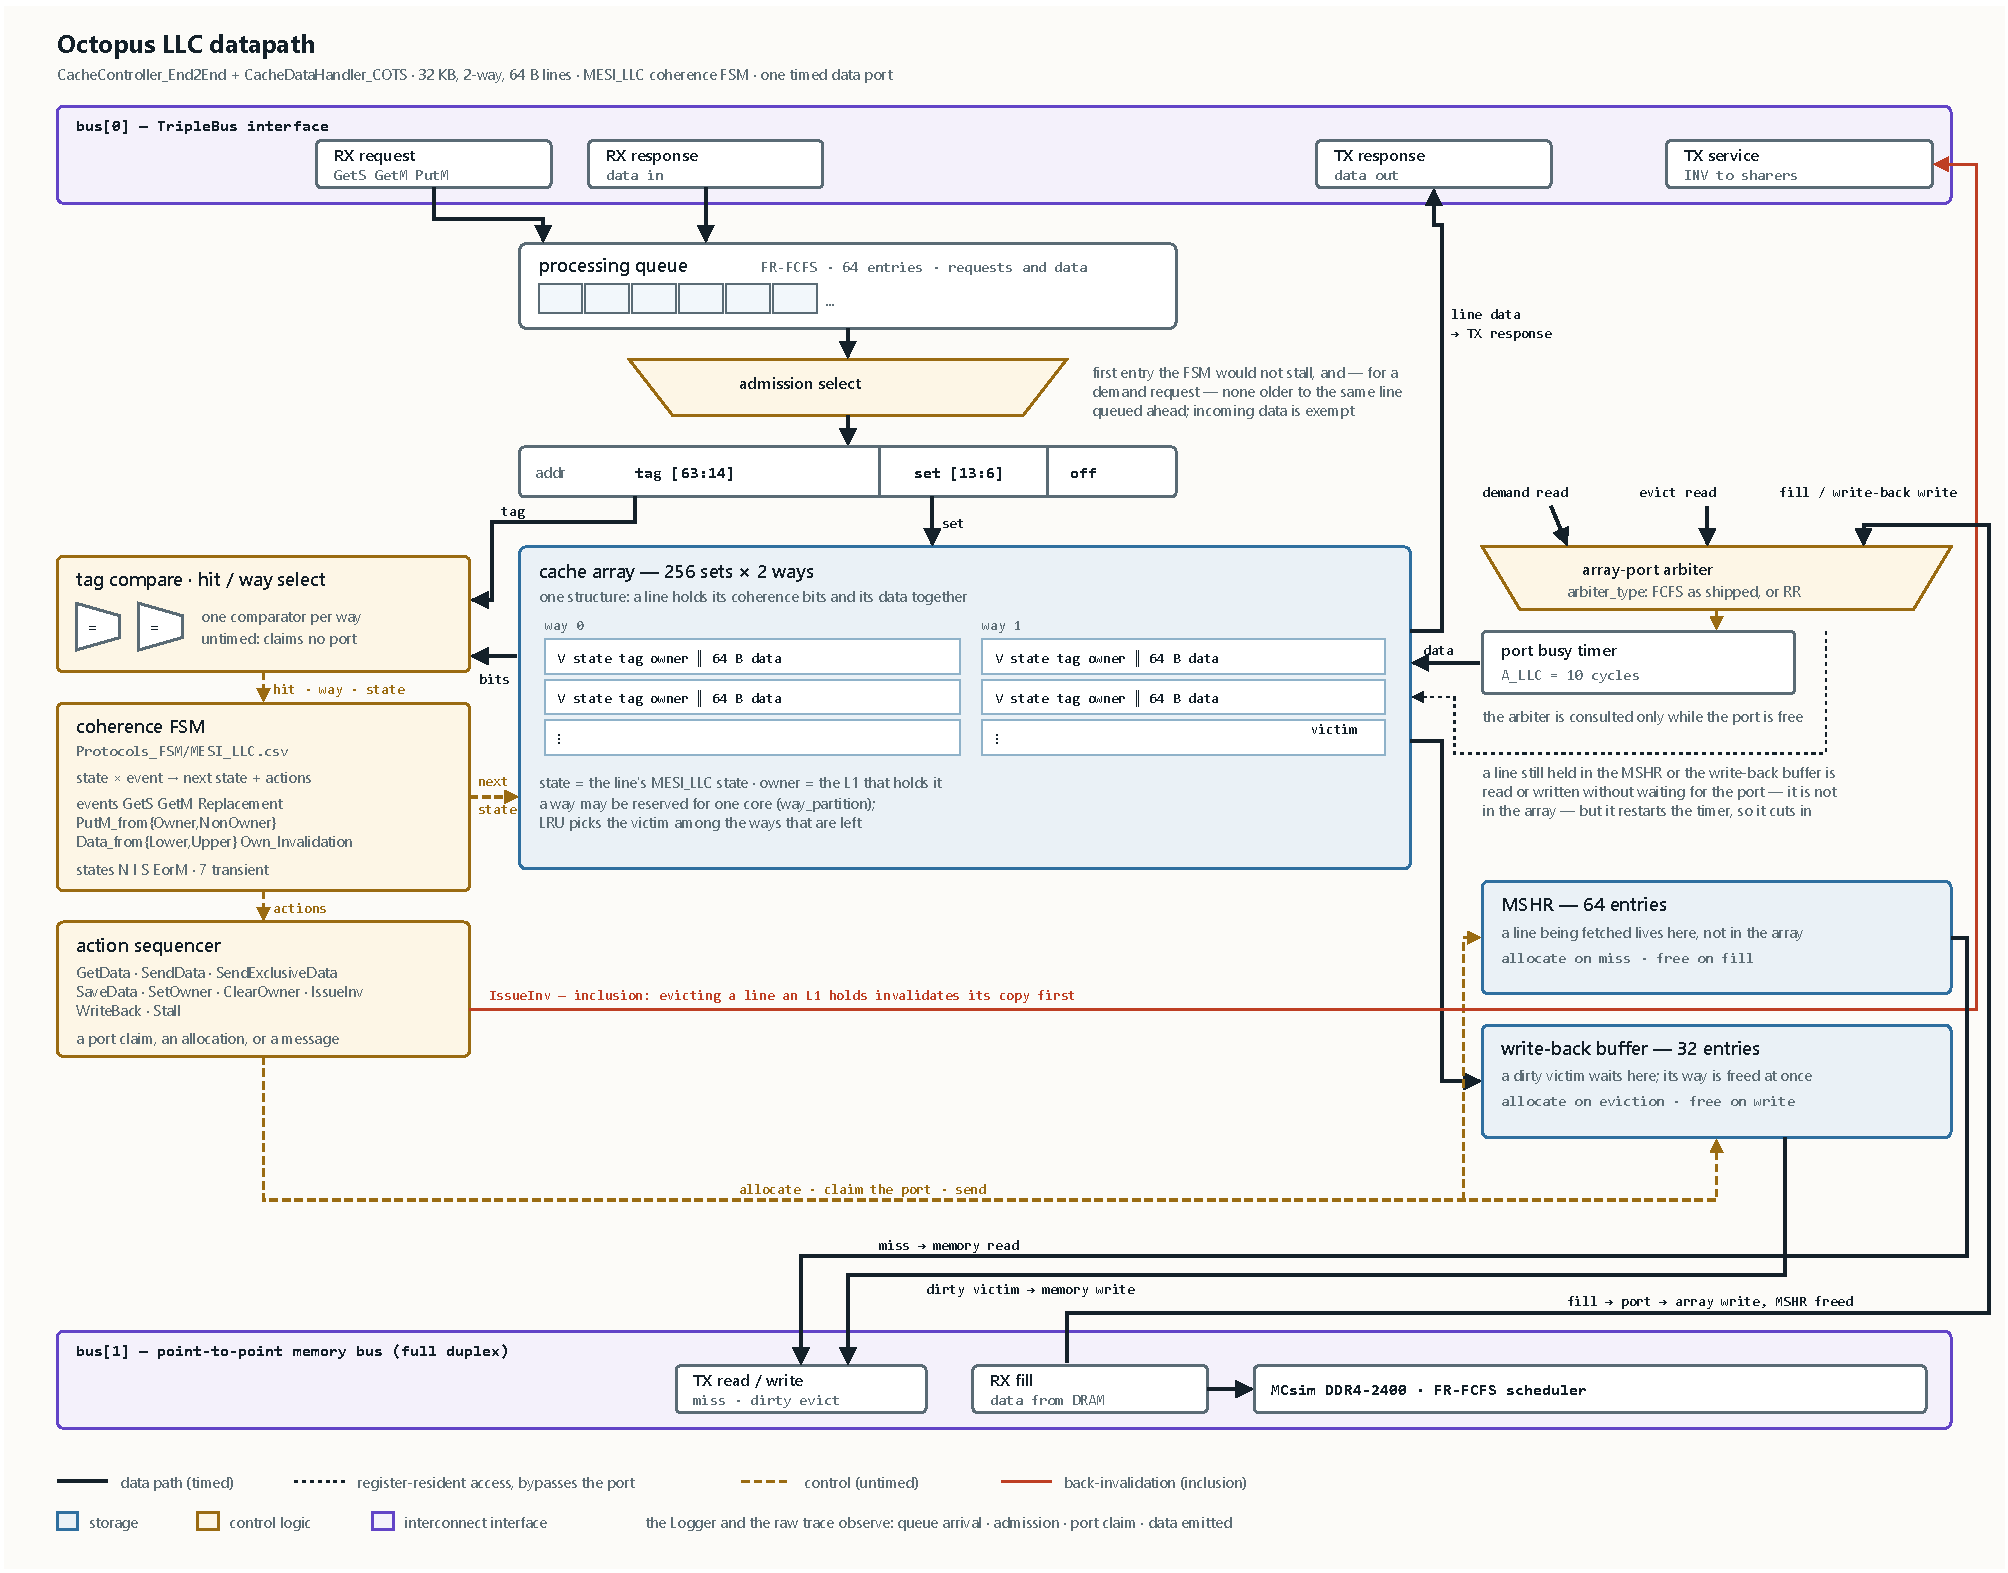
\includegraphics[width=\textwidth]{llc_architecture.pdf}
\caption[The shipped LLC as a datapath]{The shipped LLC as a datapath: \code{CacheController\_End2End}
with \code{CacheDataHandler\_COTS}, 32\,KB, 2-way, 64\,B lines, the \code{MESI\_LLC} FSM and
one timed data port. Bus interfaces on top, control on the left, the single array in the
middle read by an untimed bits path and a timed data port on the right, MSHR and write-back
buffer beside it, the memory bus below.}\label{fig:llc-architecture}\end{figure}

\Cref{fig:llc-architecture} follows the model rather than a textbook cache. The address splits
into tag, set and offset, and the set indexes \emph{one} array: in Octopus a line carries its
coherence bits and its data together, so there is no separate tag array. That array is read two
ways, and the difference matters for every latency the simulator reports. Reading a line's bits
--- the tag compare, the state the FSM needs --- is \textbf{untimed} and claims nothing. Reading
or writing its \textbf{data} goes through a single port, which demand reads, eviction reads and
fill or write-back writes contend for through the round-robin arbiter, and which is then busy
for \code{A\_LLC} cycles. A line that currently sits in the MSHR or the write-back buffer is read
without waiting for that port, because it is not in the array yet --- the dotted bypass --- but
it still restarts the busy timer, which is why such accesses cut in ahead of one already in
progress.

Control is the dashed amber layer: the line state and the decoded event enter the coherence
FSM, whose next state is written back into the line and whose actions become port claims,
buffer allocations and messages. A miss allocates in the MSHR and leaves on the memory bus; a
victim moves to the write-back buffer and frees its way at once; and because the cache is
inclusive, the FSM's \act{IssueInv} on an eviction invalidates the copy in whichever L1 holds the
line --- the red path, and the reason a task whose working set fits in its own private cache can
still be disturbed by other cores (\cref{ch:tasks-and-demo}).

\section{A read hit}

\figwide{llc_hit_path.pdf}{A read or write hit --- a \code{GetS} or \code{GetM} that finds the
line in a stable state --- from the request's arrival on the bus to its data leaving on the
response lane, in ten numbered steps.}{fig:llc-hit}

Steps 4--6 --- tag compare, FSM, sequencer --- take no simulated time. What a hit pays for is the
wait in the processing queue (1--3), the wait for the port (7), and then the \code{A\_LLC}-cycle
access itself (8--9). The figure draws the case where the LLC serves the data: the line is valid
in the array and no L1 owns it (\state{I} or \state{S} in \code{MESI\_LLC.csv}). The third case,
a hit on a line an L1 holds in \state{EorM}, does not use the port at all: the owner answers the
\code{GetS} on the bus with \act{Data2Both}, and the LLC only saves that copy
(\state{S\_d} $\rightarrow$ \act{SaveData} $\rightarrow$ \state{S}); on a \code{GetM} the owner
hands the line straight to the requester and the LLC merely rewrites the owner bits.

\section{A write hit}

\figwide{llc_write_hit.pdf}{The write hit on its own. The path is the read hit's; what is new
is the branch marked 5b --- the FSM's \code{SetOwner} written back into the line's bits over the
dashed control wire, untimed --- and the plain-data response.}{fig:llc-write-hit}

A write hit differs from a read hit in what the FSM does, not in the path: the \code{GetM} gets
plain data where a \code{GetS} gets exclusive data, and the FSM also rewrites the owner bits.
Nothing else changes --- in particular the LLC sends \textbf{no} invalidation: on the snooping
bus every sharer sees the \code{GetM} itself and drops its copy
(\state{S} + \code{Other\_GetM} $\rightarrow$ \state{I}), so \act{IssueInv} is reserved for
evictions.

\section{A read miss into a free way}

\figwide{llc_read_miss.pdf}{A read miss in the simplest case: the set still has a free way, so
nothing is evicted. The request's own path in teal; the array write of the fill, off the
critical path, dashed.}{fig:llc-read-miss}

The request takes the same first six steps and then diverges at the tag compare: the FSM's
\act{GetData} allocates an MSHR entry, the read leaves on \code{bus[1]}, and the line waits in the
MSHR --- not the array --- until DRAM answers. When the fill is processed the response goes out
on TX response at once, carrying the data from the fill message; the write into the free way
--- which contends for the port like any other array access and frees the MSHR --- runs in
parallel, off the requester's critical path. Because no victim is chosen, the write-back buffer
and the red inclusion path are never touched. A write miss takes the identical route with a
\code{GetM} in place of the \code{GetS}.

\section{A miss that evicts}

\figwide{llc_miss_evict.pdf}{A miss into a \emph{full} set: the requested line in teal, the
evicted victim in amber. The victim is chosen when the fill is written, and its exit is a
coherence transaction of its own.}{fig:llc-miss-evict}

Two things in \cref{fig:llc-miss-evict} are easy to get wrong from a textbook. First,
\textbf{the victim is chosen late}: the miss allocates an MSHR and sends the read while the full
set is left alone, and only when the fill's array write runs does the data handler pick the LRU
line among the requester's allowed ways, move it --- bits and data --- into the write-back
buffer, and put the fill in its way (\code{moveLine2WB} inside \code{updateLineData}). The
requester's data leaves on TX response right then; everything the victim costs comes afterwards
and lands on \emph{other} traffic. Second, \textbf{the victim's exit is a coherence transaction},
not a buffer drain: a \code{Replacement} is raised for it and goes through the queue and the FSM
like any request, \act{IssueInv} puts an \code{INV} on the service lane, every L1 that shares the
line drops it, the LLC receives its own \code{INV} back, and only then does \act{WriteBack} read
the line --- from the buffer, over the dotted bypass --- and send it to memory. There is no dirty
bit in the model, so every victim is written back; the code marks the spot with a \code{ToDo}.
A \code{GetM} miss evicts identically. A victim an L1 \emph{owns} adds one leg: the owner answers
the \code{INV} with its data, and that copy is what reaches memory.

Seen from the cores instead of from inside the LLC, that eviction is the whole story of
inter-core interference through an inclusive LLC; \cref{ch:tasks-and-demo} draws it as a
sequence and \cref{ch:request-end-to-end} shows what it costs the victim's next request.

\begin{wherebox}
\begin{itemize}[nosep,leftmargin=1.2em]
\item \file{src/CacheControllers/CacheController_End2End.cpp} --- the LLC controller
\item \file{src/CacheDataHandler_COTS.cpp} --- \code{updateLineData}, \code{moveLine2WB}, the port arbiter and the bypass
\item \file{Protocols_FSM/MESI_LLC.csv} --- the FSM (\cref{app:fsm-tables})
\item \file{src/Protocols/LLCMESIProtocol.cpp} --- its handler
\item \file{src/CacheControllers/CacheController.cpp} --- \code{sendInvalidationMessage}, \code{checkReplacements}
\item \file{configuration/SystemConfigurations/MultiCoreSystem.csv} --- the \code{llc\_controller.*} keys that size it
\end{itemize}
\end{wherebox}

\chapter[The coherence engine]{The coherence engine: CSV finite-state machines}\label{ch:coherence-engine}

\whatyoufind{Why a coherence protocol in Octopus is a spreadsheet and not a program; the exact
format of that spreadsheet and the one rule about it that silently breaks protocols; the
vocabulary of events a controller can see and actions it can perform; the families that ship
and how a snooping protocol differs from a directory one; and a worked example, MI, added
without a line of C++.}

\section{Coherence as data}

A cache controller's coherence logic is a finite-state machine read at start-up from a CSV
file. Rows are states, stable and transient; columns are coherence events; each cell lists the
actions and the next state for that (state, event) pair. Adding or modifying a protocol means
editing the table --- no C++ change and no recompilation. The same engine, \code{FSMReader} plus
a per-family protocol handler, drives MSI, MESI and MOESI in their snooping and directory forms,
and the predictable protocols built on Octopus (\cref{ch:introduction}).

The split pays off in code size. Because the handler only translates a small set of protocol
actions into controller actions, a protocol that extends a family it already knows costs little:
\cref{tab:loc} contrasts the lines of code per protocol with gem5's Ruby.

\begin{table}[htbp]\centering\small
\caption{Lines of code per coherence protocol, Octopus versus gem5's Ruby. In Octopus the count
is the CSV table plus the handler code specific to that protocol; MESI and MOESI extend MSI's
handler.}\label{tab:loc}
\begin{tabular}{@{}lrrrr@{}}
\toprule & MSI & MESI & MOESI & PENDULUM \\ \midrule
gem5 (Ruby) & 800 & 1400 & 1300 & 2000 \\
\textbf{Octopus} & \textbf{300} & \textbf{70} & \textbf{120} & \textbf{500} \\
\bottomrule
\end{tabular}
\end{table}

\section{The table}\label{sec:fsm-format}

\begin{figure}[htbp]\centering
\begin{adjustbox}{max width=\textwidth}% An excerpt of MESI_LLC.csv with the four things a reader must know about the format.
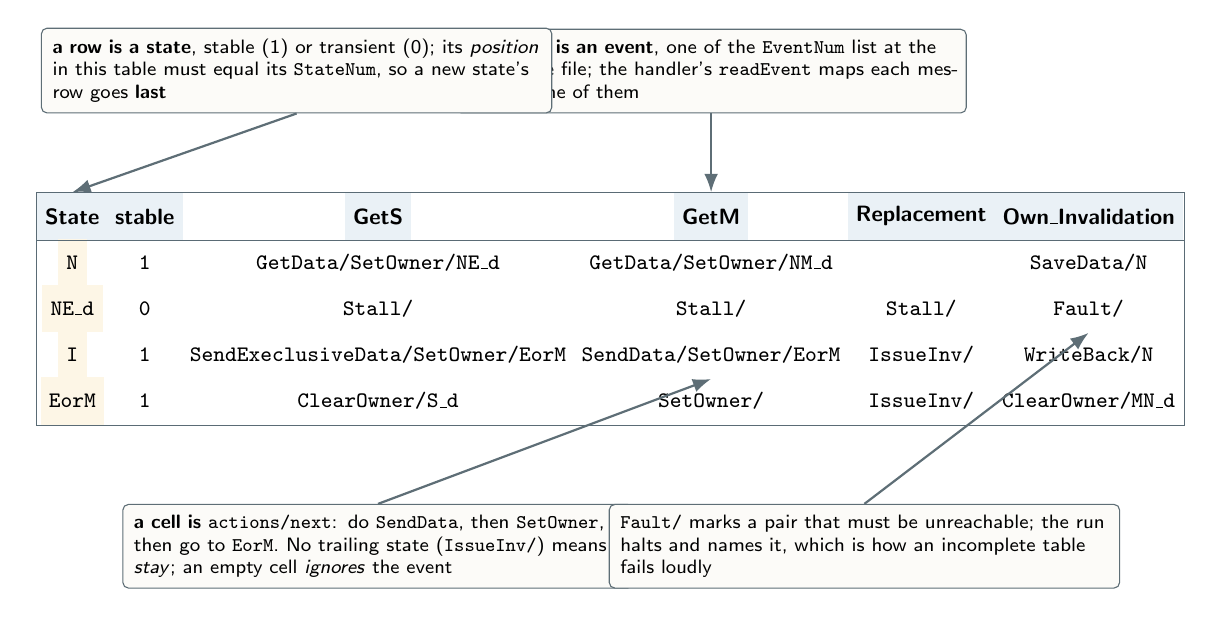
\begin{tikzpicture}[font=\sffamily\footnotesize, >=Latex,
  cell/.style={minimum height=6mm, inner sep=3pt, anchor=center, font=\ttfamily\footnotesize},
  hdr/.style={cell, fill=octmem, font=\sffamily\bfseries\footnotesize},
  st/.style={cell, fill=octctl, font=\ttfamily\bfseries\footnotesize},
  note/.style={draw=octquiet, fill=octpaper, rounded corners=2pt, inner sep=4pt, align=left, font=\sffamily\scriptsize, text width=62mm},
  pin/.style={->, octquiet, thick}]
  \matrix (m) [matrix of nodes, nodes={cell}, column sep=-\pgflinewidth, row sep=-\pgflinewidth, nodes in empty cells,
    column 1/.style={nodes={st}}, row 1/.style={nodes={hdr}}] {
    State & stable & GetS & GetM & Replacement & Own\_Invalidation \\
    N     & 1 & GetData/SetOwner/NE\_d & GetData/SetOwner/NM\_d & & SaveData/N \\
    NE\_d & 0 & Stall/ & Stall/ & Stall/ & Fault/ \\
    I     & 1 & SendExeclusiveData/SetOwner/EorM & SendData/SetOwner/EorM & IssueInv/ & WriteBack/N \\
    EorM  & 1 & ClearOwner/S\_d & SetOwner/ & IssueInv/ & ClearOwner/MN\_d \\
  };
  \draw[octrule] (m-1-1.south west) -- (m-1-6.south east);
  \draw[octrule] (m-1-1.north west) rectangle (m-5-6.south east);
  % callouts above
  \node[note, above=10mm of m-1-4.north, anchor=south] (nev) {\textbf{a column is an event}, one of the \code{EventNum} list at the top of the file; the handler's \code{readEvent} maps each message to one of them};
  \draw[pin] (nev.south) -- (m-1-4.north);
  \node[note, above=10mm of m-1-1.north, anchor=south west, xshift=-4mm] (nst) {\textbf{a row is a state}, stable (1) or transient (0); its \emph{position} in this table must equal its \code{StateNum}, so a new state's row goes \textbf{last}};
  \draw[pin] (nst.south) -- (m-1-1.north);
  % callouts below
  \node[note, below=10mm of m-5-3.south, anchor=north] (ncell) {\textbf{a cell is \code{actions/next}}: do \code{SendData}, then \code{SetOwner}, then go to \code{EorM}. No trailing state (\code{IssueInv/}) means \emph{stay}; an empty cell \emph{ignores} the event};
  \draw[pin] (ncell.north) -- (m-4-4.south);
  \node[note, below=10mm of m-5-6.south, anchor=north east, xshift=4mm] (nf) {\textbf{\code{Fault/}} marks a pair that must be unreachable; the run halts and names it, which is how an incomplete table fails loudly};
  \draw[pin] (nf.north) -- (m-3-6.south);
\end{tikzpicture}
\end{adjustbox}
\caption{An excerpt of \code{MESI\_LLC.csv} with the four things to know about the format.
\Cref{app:fsm-tables} prints every shipped table in full.}
\label{fig:fsm-annotated}
\end{figure}

A file in \file{Protocols_FSM/} has four blocks (\cref{fig:fsm-annotated}):

\begin{enumerate}
\item \textbf{Events}, numbered from 0: the columns of the transition table. For the snooping
  L1 they are exactly \evt{Load}, \evt{Store}, \evt{Replacement}, \evt{Own\_GetS},
  \evt{Own\_GetM}, \evt{Own\_PutM}, \evt{Other\_GetS}, \evt{Other\_GetM}, \evt{Other\_PutM},
  \evt{OwnData}, \evt{Invalidation} and \evt{OwnData\_Execlusive}; for the snooping LLC
  \evt{GetS}, \evt{GetM}, \evt{Replacement}, \evt{PutM\_fromOwner}, \evt{PutM\_fromNonOwner},
  \evt{Data\_fromLowerInterface}, \evt{Data\_fromUpperInterface} and \evt{Own\_Invalidation}.
\item \textbf{Actions}, numbered from 0: what a cell may ask for. The L1 offers \act{Stall},
  \act{Hit}, \act{GetS}, \act{GetM}, \act{PutM}, \act{Data2Req}, \act{Data2Both}, \act{SaveReq},
  \act{Fault} and \act{removeSavedReq}; the LLC offers \act{Stall}, \act{GetData},
  \act{SendData}, \act{SaveData}, \act{SetOwner}, \act{ClearOwner}, \act{IssueInv},
  \act{WriteBack}, \act{Fault} and \act{SendExeclusiveData}. Each type of controller offers its
  list independently of the protocol, which is what lets one controller class run several
  protocols.
\item \textbf{States}, numbered from 0, stable and transient alike. Transient names follow the
  textbook convention: \state{IS\_ad} is ``going from I to S, awaiting the bus (a) and the data
  (d)'', \state{IM\_dI} is ``going to M, data pending, but invalidated meanwhile''.
\item \textbf{The transition table}: a header row \code{State, stable, isDataValid, <events>},
  then one row per state. \code{stable} marks the stable states; \code{isDataValid} says whether
  the line's data may be read in that state. A cell is \code{Action1/Action2/NextState}. A cell
  whose last element is an action, not a state (\code{IssueInv/}), stays in the current state;
  an empty cell ignores the event; \code{Fault/} declares the pair unreachable.
\end{enumerate}

\begin{trapbox}[Row order is the state number]
\code{FSMReader} indexes transition rows by \emph{position}, not by name. When you add a state,
its row must be appended \textbf{last}, so that its position matches the number you gave it in
the state list. Put it anywhere else and the FSM silently runs another state's transitions ---
no error, just wrong results. This is the single most likely way a protocol edit goes wrong.
\end{trapbox}

\paragraph{Reading a cell.} In \cref{fig:fsm-annotated}, state \state{I} (the LLC has the line,
no L1 owns it) on \evt{GetM} reads \code{SendData/SetOwner/EorM}: send the data to the
requester, record it as the owner, and move to \state{EorM}. The same state on
\evt{Replacement} reads \code{IssueInv/}: broadcast an invalidation and stay --- the eviction
completes later, when the LLC's own copy of that invalidation comes back as
\evt{Own\_Invalidation} and the cell \code{WriteBack/N} runs. \Cref{ch:llc-datapath} draws those
two paths.

\paragraph{Fault is an audit.} A cell of \code{Fault/} means ``this (state, event) should be
unreachable''. The handler halts the run and reports the pair rather than mis-routing silently.
That is what makes a protocol auditable: an incomplete or wrong table fails loudly on the first
trace that exercises the hole, and the Debugger's transition trace (\cref{ch:monitoring}) shows
the exact sequence that reached it.

\section{Stable and transient states}

A snooping protocol on a split-transaction bus is mostly transient states. A request is issued
(\act{GetS}), travels the request lane, is seen back by its own issuer (\evt{Own\_GetS}: the
line is now ordered on the bus), and some time later the data arrives (\evt{OwnData}); between
those moments other cores' requests to the same line are seen (\evt{Other\_GetS},
\evt{Other\_GetM}) and may have to be remembered (\act{SaveReq}) and answered when the data
finally comes (\act{Data2Req}, \act{Data2Both}). Each such interleaving is a row. The shipped
MESI L1 has 4 stable and 20 transient states; its LLC 4 stable and 7 transient
(\cref{app:fsm-tables}).

The LLC side uses states a textbook does not name. \state{N} is ``not present'';
\state{EorM} is ``an L1 owns this line, I do not know in which of E or M''; \state{MN\_d} is
``evicting, waiting for the owner's data''. They exist because the LLC is inclusive and tracks
one owner per line, and they are where most of the subtle behaviour of \cref{ch:llc-datapath}
lives.

\section{Snooping and directory}

\begin{figure}[htbp]\centering
\begin{adjustbox}{max width=\textwidth}% One GetM from core A while core B shares the line: snooping (left) and directory (right).
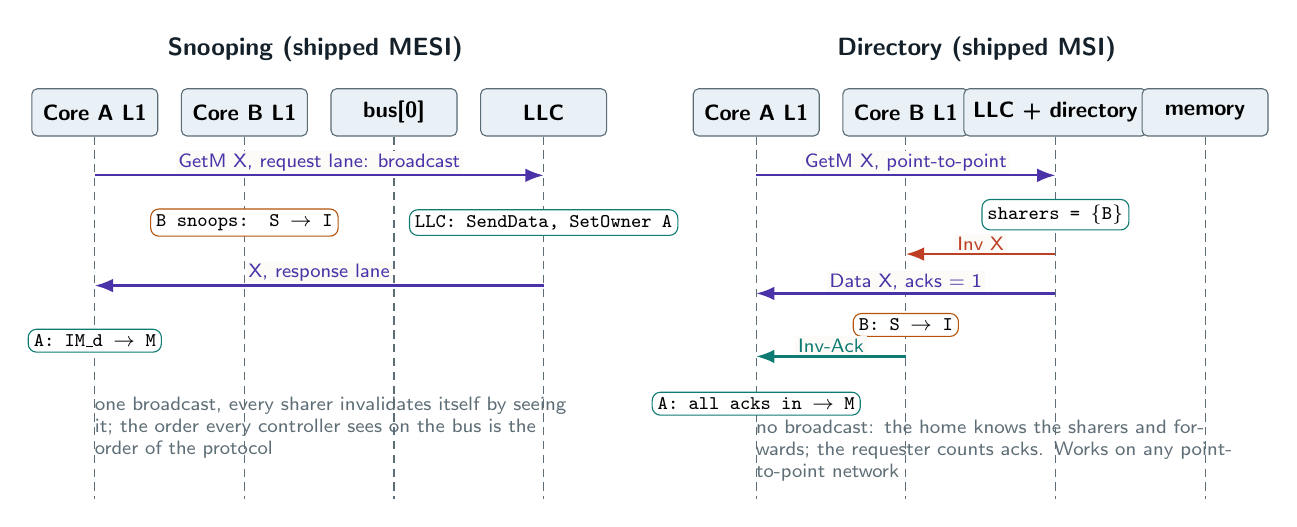
\begin{tikzpicture}[font=\sffamily\scriptsize, >=Latex,
  head/.style={draw=octrule, fill=octmem, rounded corners=2pt, minimum width=16mm, minimum height=6mm, font=\sffamily\footnotesize\bfseries},
  life/.style={octquiet, densely dashed},
  m/.style={->, thick},
  lbl/.style={font=\sffamily\scriptsize, fill=octpaper, inner sep=1pt},
  pill/.style={draw, fill=white, rounded corners=3pt, inner sep=2pt, font=\ttfamily\scriptsize},
  ttl/.style={font=\sffamily\small\bfseries, text=octink}]
  % ---------- snooping ----------
  \begin{scope}
    \node[ttl] at (28mm, 8mm) {Snooping (shipped MESI)};
    \foreach \x/\n/\t in {0/A/Core A L1, 19/B/Core B L1, 38/bus/bus[0], 57/llc/LLC}
      { \node[head] (s\n) at (\x mm, 0) {\t}; \draw[life] (s\n.south) -- ++(0,-46mm); }
    \draw[m, octpurple] (sA) ++(0,-8mm) -- node[lbl, above] {GetM X, request lane: broadcast} ++(57mm, 0);
    \node[pill, draw=octamber] at (19mm, -14mm) {B snoops: S $\rightarrow$ I};
    \node[pill, draw=octteal] at (57mm, -14mm) {LLC: SendData, SetOwner A};
    \draw[m, octpurple] (sllc) ++(0,-22mm) -- node[lbl, above] {X, response lane} ++(-57mm, 0);
    \node[pill, draw=octteal] at (0mm, -29mm) {A: IM\_d $\rightarrow$ M};
    \node[align=left, text=octquiet, text width=60mm] at (30mm, -40mm) {one broadcast, every sharer invalidates itself by seeing it; the order every controller sees on the bus is the order of the protocol};
  \end{scope}
  % ---------- directory ----------
  \begin{scope}[xshift=84mm]
    \node[ttl] at (28mm, 8mm) {Directory (shipped MSI)};
    \foreach \x/\n/\t in {0/A/Core A L1, 19/B/Core B L1, 38/home/LLC + directory, 57/mem/memory}
      { \node[head] (d\n) at (\x mm, 0) {\t}; \draw[life] (d\n.south) -- ++(0,-46mm); }
    \draw[m, octpurple] (dA) ++(0,-8mm) -- node[lbl, above] {GetM X, point-to-point} ++(38mm, 0);
    \node[pill, draw=octteal] at (38mm, -13mm) {sharers = \{B\}};
    \draw[m, octred] (dhome) ++(0,-18mm) -- node[lbl, above] {Inv X} ++(-19mm, 0);
    \draw[m, octpurple] (dhome) ++(0,-23mm) -- node[lbl, above] {Data X, acks = 1} ++(-38mm, 0);
    \node[pill, draw=octamber] at (19mm, -27mm) {B: S $\rightarrow$ I};
    \draw[m, octteal] (dB) ++(0,-31mm) -- node[lbl, above] {Inv-Ack} ++(-19mm, 0);
    \node[pill, draw=octteal] at (0mm, -37mm) {A: all acks in $\rightarrow$ M};
    \node[align=left, text=octquiet, text width=60mm] at (30mm, -43mm) {no broadcast: the home knows the sharers and forwards; the requester counts acks. Works on any point-to-point network};
  \end{scope}
\end{tikzpicture}
\end{adjustbox}
\caption{One \code{GetM} from core A while core B shares the line, under the shipped snooping
MESI (left) and the shipped directory MSI (right).}
\label{fig:snoop-vs-directory}
\end{figure}

The two families differ in who learns about a request (\cref{fig:snoop-vs-directory}). Under
snooping every L1 sees every request on the request lane and acts on its own copy; the order of
the bus is the order of the protocol, and the LLC's job is to supply data when no L1 owns the
line and to track the owner when one does. Under a directory the home --- the LLC-side
\code{CacheControllerDirectory} --- keeps a sharer list per line, forwards each request only to
the caches that need to act, and the requester counts the acknowledgements; nothing is
broadcast, which is what lets a directory run on a point-to-point network such as the mesh
(\cref{ch:interconnects}). The same controllers, queues and data handlers serve both; only the
protocol handler and the tables differ.

\begin{table}[htbp]\centering\small
\caption{The protocol families that ship, and the preset that selects each. The L1 and LLC
tables of a family are a matched pair.}\label{tab:families}
\footnotesize
\begin{tabularx}{\textwidth}{@{}p{0.17\textwidth}p{0.27\textwidth}p{0.2\textwidth}Y@{}}
\toprule family & L1 table & LLC table & selected by \\ \midrule
snoop MSI & \file{MSI_splitBus_snooping} & \file{MSI_LLC} & \file{MultiCoreSystem_Snoop.csv} \\
snoop MESI & \file{MESI_splitBus_snooping} & \file{MESI_LLC} & \file{MultiCoreSystem.csv} (the default) \\
snoop MOESI & \file{MOESI_splitBus_snooping} & \file{MOESI_LLC} & no preset \\
directory MSI & \file{MSI_directory} & \file{MSI_LLC_directory} & \file{MultiCoreSystem_Directory.csv} \\
directory MESI, MOESI & \file{MESI_directory}, \file{MOESI_directory} & \file{MESI_LLC_directory}, \file{MOESI_LLC_directory} & no preset \\
predictable & \file{PMSI}, \file{PMESI}, \file{PMSI_asterisk}, \file{PMESI_asterisk}, \file{Pendulum} & their \file{_LLC} tables & research configurations \\
\bottomrule
\end{tabularx}
\end{table}

\begin{trapbox}[{A protocol is five keys, and the tables are a matched pair}]
Selecting a protocol sets the controller class, the L1 and LLC \code{protocol\_type} and the L1
and LLC \code{fsm\_filename} together (\cref{ch:configuration}). A MESI L1 with an MSI LLC
faults with ``Wrong destination''; overriding some of the five from the command line faults or
crashes. Switch by preset, not by hand.
\end{trapbox}

\section{A worked example: MI without C++}

MI is the simplest coherence protocol: a line is either Invalid or Modified, so every access,
even a load, takes it exclusive. It is MSI with the \state{S} state and its transients removed
and \evt{Load} behaving like \evt{Store}: 9 states instead of 22. Because MI uses only a subset
of MSI's events and actions, it runs on the existing \code{SNOOP\_MSI} handler and the existing
\code{MSI\_LLC}: the entire protocol is one CSV, \file{Protocols_FSM/MI_splitBus_snooping.csv}.

\begin{table}[htbp]\centering\small
\caption{The two stable rows of \code{MI\_splitBus\_snooping.csv}; the columns not shown are
those of MSI.}\label{tab:mi-rows}
\begin{tabular}{@{}>{\ttfamily}l>{\ttfamily}c>{\ttfamily}c>{\ttfamily}l>{\ttfamily}l>{\ttfamily}c>{\ttfamily}l>{\ttfamily}l@{}}
\toprule
\normalfont\textbf{State} & \normalfont\textbf{stable} & \normalfont\textbf{isDataValid} & \normalfont\textbf{Load} & \normalfont\textbf{Store} & \ldots & \normalfont\textbf{OwnData} & \normalfont\textbf{Invalidation} \\ \midrule
I & 1 & 0 & GetM/IM\_ad & GetM/IM\_ad & \ldots & Fault/ & \\
M & 1 & 1 & Hit/ & Hit/ & \ldots & Fault/ & Data2Req/I \\
\bottomrule
\end{tabular}
\end{table}

Selecting it is one override on top of the MSI preset:

\begin{lstlisting}[style=shell]
./build/Octopus_Simulator -s MultiCoreSystem \
  -p "workload_path(s)=BMs/eembc-traces/mi_pingpong/" \
  -p "cache_controller[*].fsm_filename(s)=MI_splitBus_snooping"
\end{lstlisting}

On the \code{mi\_pingpong} toy workload, where cores 0 and 1 repeatedly read one line, MESI lets
the two cores share it and finishes in 332 cycles; MI makes the line ping-pong exclusively
between them and finishes in 482. The Logger shows the cost; the Debugger's address-filtered
transition trace shows the cause --- \code{I --Load--> IM\_ad} under MI against
\code{I --Load--> IS\_ad} under MESI. One new file, one override, no compiler.

\begin{wherebox}
\begin{itemize}[nosep,leftmargin=1.2em]
\item \file{Protocols_FSM/} --- the tables, one CSV per agent
\item \file{header/FSMReader.h}, \file{src/FSMReader.cpp} --- the parser and \code{getTransition}
\item \file{src/Protocols/MSIProtocol.cpp}, \file{src/Protocols/MESIProtocol.cpp}, \file{src/Protocols/MOESIProtocol.cpp} --- the snooping L1 handlers
\item \file{src/Protocols/LLCMSIProtocol.cpp}, \file{src/Protocols/LLCMESIProtocol.cpp} --- the snooping LLC handlers (MOESI's LLC runs on the MESI handler)
\item \file{src/Protocols/MSIDirectory.cpp}, \file{src/Protocols/MESIDirectory.cpp}, \file{src/Protocols/MOESIDirectory.cpp} --- the directory L1 handlers
\item \file{src/Protocols/LLCMSIDirectory.cpp}, \file{src/Protocols/LLCMESIDirectory.cpp}, \file{src/Protocols/LLCMOESIDirectory.cpp} --- the directory home handlers
\item \file{docs/AddingAProtocol.md} --- the MI example in full
\item \file{demo_protocol.sh} --- runs it
\end{itemize}
\end{wherebox}

\chapter{A request, end to end}\label{ch:request-end-to-end}

\whatyoufind{One memory request followed from the core that issues it to the core that
retires it, drawn on the system as shipped and on a time axis; the Logger stamp at every hop;
and, from those stamps, the exact definition of every column of a \code{LatencyReport}. This is
the chapter to have open the first time you read a report: a total tells you a core was slow,
the columns tell you which shared resource made it slow, and this is what each column is.}

\section{The journey}

A core issues a \code{Message}. Its L1 admits it, looks the line up and, on a miss, puts a
\code{GetS} (read) or \code{GetM} (write) on the request lane of \code{bus[0]}, where the arbiter
elects it. Every other L1 snoops it; the LLC admits it into its queue. If the LLC has the line
and no L1 owns it, the data is emitted when the array port is granted; if an L1 owns it, that
L1 answers on the response lane instead; if the LLC does not have it, a read leaves on
\code{bus[1]}, DRAM serves it, the fill comes back to the front of the LLC's queue and the
response is emitted from it. The response travels the response lane to the requesting L1, which
fills and hands the data to the core.

\figpage{system_end_to_end.pdf}{The system as shipped with one LLC \emph{miss} from core 0
routed through it. Each hop carries the colour of the \code{LatencyReport} column that measures
it (amber: waiting; purple: a bus transfer; teal: being served) and the number of the Logger
stamp that bounds it, \ding{172}--\ding{181} being the report's nine latency columns in order; the
side panel lists the stamp pair behind every column.}{fig:system-miss}

\figpage{system_end_to_end_hit.pdf}{The same system with an LLC \emph{hit} from core 0. The route
stops at the LLC's array port, where the data is emitted at the grant; the memory bus and DRAM
are not on the path, so \col{L2-DRAM Bus} and \col{DRAM} are 0.}{fig:system-hit}

\Cref{fig:system-miss,fig:system-hit} are the same drawing with the two routes. Three things
on them are worth saying in words. The other cores' L1s see every request on the request lane,
and when one of them owns the line it answers on the response lane in the LLC's place, its
stamps then standing in for the LLC's. The service lane carries the LLC's back-invalidations on
an eviction and is on neither request's path. And a hit's \col{L2 Access} ends at the port
\emph{grant}: the data leaves then, and the read's \code{A\_LLC} cycles on the port are paid by
whoever waits for the port next --- their \col{L2 Access}, or a fill's write.

\section{The stamps}

At each hop the component stamps a Logger checkpoint: an \stamp{ENTER} when it takes custody of
the request, a \stamp{SERVICE} when it begins the actual work, an \stamp{EXIT} when it hands the
request on. Every stamp names the component's \emph{role} (\code{CPU}, \code{L1},
\code{REQ\_BUS}, \code{RESP\_BUS}, \code{LLC}, \code{MEM\_BUS}, \code{DRAM}) and is taken in the
originating core's clock, so a request's timeline is one ordered list of self-describing events
and the columns are differences of \emph{named} stamps, never inferences from position
(\cref{ch:monitoring} has the mechanism). \Cref{tab:stamps} lists who stamps what.

\begin{table}[htbp]\centering\small
\caption{Where each Logger stamp is taken.}\label{tab:stamps}
\begin{tabularx}{\textwidth}{@{}>{\ttfamily}p{0.3\textwidth}Y@{}}
\toprule \normalfont stamp & taken by \\ \midrule
CPU.ENTER & \code{CPU::addRequest}: the request is issued (and bound to its core) \\
L1.ENTER & \code{BaseController::processLogic} when an L1 admits a request from below \\
REQ\_BUS.EXIT & \code{BusController::broadcast} on \code{bus[0]}: the request is transmitted \\
LLC.ENTER & \code{BaseController::processLogic} when the LLC admits the bus request \\
MEM\_BUS.EXIT & \code{BusController} on \code{bus[1]}, once in each direction \\
DRAM.ENTER, DRAM.EXIT & \code{MainMemoryController}: request arrives, data leaves after \key{m\_memory\_latency}. MCsim stamps neither \\
LLC.SERVICE, LLC.EXIT & \code{hitAction} / \code{removePendingAndRespond}: port granted; response emitted \\
L1.SERVICE, L1.EXIT (before RESP\_BUS.EXIT) & \code{performWriteBack} when an \emph{owning} L1 supplies another core's request; the responder is then that L1, not the LLC \\
RESP\_BUS.EXIT & \code{BusController::send} on \code{bus[0]}: the response is transmitted \\
CPU.EXIT & \code{CPU::checkReceiveBuffer}: delivered; triggers the report row \\
\bottomrule
\end{tabularx}
\end{table}

\figpage{request_end_to_end.pdf}{The same two routes on a time axis: an LLC hit and an LLC
miss, with the nine \code{LatencyReport} columns bracketed between the Logger stamps that
bound them. Ticks are in order, not to scale. Below the miss axis, the array write of the fill
runs alongside the response and lands in no column.}{fig:request-timeline}

\section{The columns}

\begin{table}[htbp]\centering\small
\caption{The \code{LatencyReport} columns, in report order, as differences of stamps. The
nine latency columns tile exactly to \col{Total}; a stamp a request never reaches makes its
column 0.}\label{tab:columns}
\begin{tabularx}{\textwidth}{@{}lY@{}}
\toprule column & definition \\ \midrule
\col{CPU Latency} & \stamp{CPU.ENTER} $-$ \col{Ready Cycle}: the wait inside the core before the request could issue (the out-of-order window). Lies \emph{before} Total \\
\col{L1 Stall} & \stamp{L1.ENTER} $-$ \stamp{CPU.ENTER} \\
\col{Request Bus} & \stamp{REQ\_BUS.EXIT} $-$ \stamp{L1.ENTER}: the L1's miss handling and its wait for the request lane \\
\col{L2 Stall} & \stamp{LLC.ENTER} $-$ \stamp{REQ\_BUS.EXIT}: the wait in the LLC's queue \\
\col{L2 Access} & hit: \stamp{LLC.SERVICE} $-$ \stamp{LLC.ENTER}, the wait for the array port; miss: \stamp{LLC.SERVICE} $-$ \stamp{MEM\_BUS.EXIT}$_2$, the fill's turn at the front of the queue, typically one cycle \\
\col{Response Bus} & \stamp{RESP\_BUS.EXIT} $-$ \stamp{LLC.EXIT}: the clean response-lane leg \\
\col{L2-DRAM Bus} & miss: (\stamp{DRAM.ENTER} $-$ \stamp{LLC.ENTER}) $+$ (\stamp{MEM\_BUS.EXIT}$_2$ $-$ \stamp{DRAM.EXIT}): one column over two hops, out and back \\
\col{DRAM} & miss: \stamp{DRAM.EXIT} $-$ \stamp{DRAM.ENTER} \\
\col{L1 Access} & \stamp{CPU.EXIT} $-$ $\max$(\stamp{L1.ENTER}, \stamp{RESP\_BUS.EXIT}): an L1 hit's own service, or the fill and hand-off after the response-lane grant \\
\col{Total} & \stamp{CPU.EXIT} $-$ \stamp{CPU.ENTER} $=$ the sum of the eight stage columns above (CPU Latency excluded) \\
\col{Effective} & \stamp{CPU.EXIT} $-$ $\max$(previous request's finish, \stamp{CPU.ENTER}): the part of Total not overlapped with the previous request; its mean is the per-core average, its sum the true added execution time \\
\col{Oldest} & \stamp{CPU.EXIT} $-$ the cycle this request became the oldest outstanding request of its core; 0 if it never was. At OoO$=1$ it equals Total \\
\bottomrule
\end{tabularx}
\end{table}

Three things in \cref{tab:columns} are easy to misread from the names alone.

\paragraph{L2 Access means two different waits.} On a hit it ends at the array-port grant, not
after \code{A\_LLC} cycles: the data is emitted at the grant, and the port's busy time is paid by
whoever waits for the port next. On a miss it is the fill's turn at the LLC: each cycle one
message moves from the memory-side RX into the \emph{front} of the processing queue, a data
message is always ready, and every ready message is handled that same cycle --- so typically a
single cycle, plus any backlog in that one FIFO, and never a wait behind queued demand
requests. The response is emitted the moment the fill is processed, carrying the data from the
fill message; the array write claims the port afterwards, in parallel. That write is the real
``L2 access'' of a miss, \cref{fig:request-timeline} draws it below the axis, and it lands in no
report column (the \code{ARRAY} lane of the visualizer shows it).

\paragraph{L2-DRAM Bus and DRAM depend on the memory model.} With \code{MainMemoryController}
the DRAM stamps exist and \col{L2-DRAM Bus} is the two memory-bus legs either side of the DRAM
service. MCsim stamps no DRAM events, so there \col{L2-DRAM Bus} becomes ``LLC admit
$\rightarrow$ read leaves on \code{bus[1]}'' and \col{DRAM} becomes the whole \code{bus[1]} round
trip, return leg included. Nothing of the round trip is lost, but the split moves.

\paragraph{A cache-to-cache supply substitutes the responder.} When the LLC never emits because
the line's owner answered on the bus, the last \stamp{L1.SERVICE}/\stamp{L1.EXIT} strictly before
\stamp{RESP\_BUS.EXIT} become the responder milestones, and the responder's \stamp{SERVICE}
replaces \stamp{LLC.ENTER} as the admission anchor --- the owner snoops the request off the bus
and may answer before the LLC admits it, so the LLC's admission is not on the data path. Then
\col{L2 Stall} is the wait for the owner, \col{L2 Access} its service, and \col{Response Bus}
still \stamp{RESP\_BUS.EXIT} $-$ responder \stamp{EXIT}. If no responder stamp exists at all, the
whole admit-to-grant interval is folded into \col{L2 Access} so the columns keep tiling, and the
run's stderr counts the request as \code{noresp}.

\section{Checking a column}

The columns tile to \col{Total} on every row by construction, and the simulator says so: the
\code{EVENT-PATH} line on stderr at the end of a run reports how many requests tiled, how
many did not, and how many had no responder. When a column looks wrong,
\env{OCTOPUS\_EVENT\_DUMP}\code{=N} prints the raw timeline --- every stamp with its role and
cycle --- of the first $N$ requests whose Total exceeds 100 cycles or that crossed the memory
bus; \env{OCTOPUS\_EVENT\_DUMP\_MIN}\code{=<cycles>} raises the threshold to isolate one outlier
row seen in a report. The seven \emph{mechanism tracker} columns that follow \col{Oldest} in the
report (the line's state when the request arrived at the LLC, whether the per-line gate held
it, how many younger responses and array accesses went ahead of it) attribute a stall to its
cause; \cref{ch:monitoring} defines them.

\begin{wherebox}
\begin{itemize}[nosep,leftmargin=1.2em]
\item \file{src/Logger.cpp} --- the stamps, \code{finalizeEvents} and the ``Report: the event timeline is the sole decomposition'' block that computes every column
\item \file{header/Logger.h} --- the \code{Role} and \code{Phase} enums
\item \file{docs/Logger.md} --- the same material as a reference
\item \file{tutorial/00-setup-and-first-run/README.md} --- reading a first report
\end{itemize}
\end{wherebox}

\chapter{Interconnects and arbitration}\label{ch:interconnects}

\whatyoufind{The three-part model every interconnect is built from; the bus family that the
shipped systems use, with its lanes, latencies and back-pressure; the three arbiters and the
one rule they share; the mesh and the single-switch NoC, with what they do and do not model
today; and where each of these is a plug-in.}

\section{Topology, controller, interfaces}

\figmed{Interconnect2.pdf}{An interconnect is a topology that creates a connection map and
instantiates one controller and the interfaces; the interfaces are the queues that hold
messages at each node; the controller moves messages between interfaces according to the map
and the configured latencies.}{fig:interconnect}{0.5}

An interconnect has two parts (\cref{fig:interconnect}). The \emph{topology}
(\code{InterconnectTopology}) is a set of message-holding interfaces plus a \emph{connection
map} describing who talks to whom. The \emph{controller} (\code{InterconnectController}) moves
messages between interfaces, and its arbiter resolves contention on shared links. Swapping the topology and controller pair yields a point-to-point
link, a unified, split or triple bus, a mesh or a NoC; swapping the arbiter yields FCFS,
round-robin or TDM. The controllers on either side see only interfaces, so nothing else in the
system changes.

Interconnects have their own clock: \key{m\_clk\_period} is 50 for every bus and mesh against
100 for the cores, so an interconnect steps twice per core cycle. The reason is resolution, not
speed: the periods are the units the \code{ClockManager} schedules in (\cref{ch:system-organization}),
and an interconnect that ticks between two core ticks can arbitrate a lane and deliver what it
carries within the same core cycle, so a request that wins the lane is at the LLC's queue one
core cycle after it was issued, and transfer times can be set in half core cycles. A transfer
occupies a link for \key{m\_request\_latency} (2) interconnect ticks for a request and
\key{m\_response\_latency} (5) for data: one core cycle and two and a half, the 2- and 5-tick
slots the visualizer draws. Both are configuration keys, so a slower link is a number, not a
clock change.

\section{The bus family}

\begin{figure}[htbp]\centering
\begin{adjustbox}{max width=\textwidth}% The three shipped interconnect shapes between the L1s and the LLC.
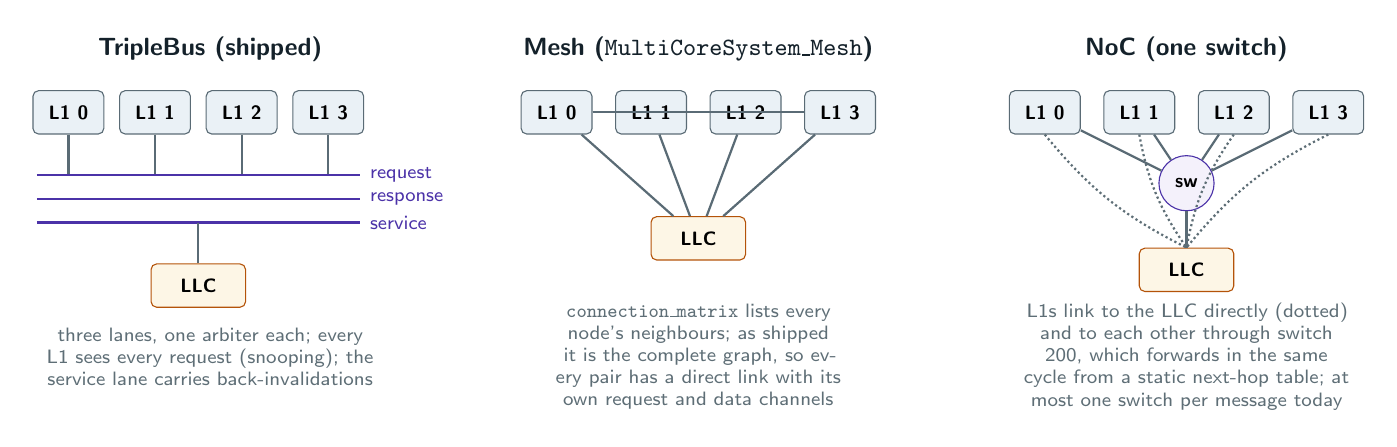
\begin{tikzpicture}[font=\sffamily\scriptsize, >=Latex,
  n/.style={draw=octrule, fill=octmem, rounded corners=2pt, minimum width=9mm, minimum height=5.5mm, font=\sffamily\scriptsize\bfseries},
  llc/.style={n, fill=octctl, draw=octamber, minimum width=12mm},
  sw/.style={draw=octpurple, fill=octio, circle, minimum size=7mm, font=\sffamily\scriptsize\bfseries},
  lane/.style={octpurple, thick},
  link/.style={octrule, thick},
  ttl/.style={font=\sffamily\small\bfseries, text=octink},
  sub/.style={font=\sffamily\scriptsize, text=octquiet, align=center, text width=44mm}]
  % ---- TripleBus ----
  \begin{scope}
    \node[ttl] at (18mm, 14mm) {TripleBus (shipped)};
    \foreach \i in {0,1,2,3} { \node[n] (b\i) at (\i*11mm, 6mm) {L1 \i}; \draw[link] (b\i.south) -- (\i*11mm, -2mm); }
    \foreach \y/\t in {-2/request, -5/response, -8/service} { \draw[lane] (-4mm, \y mm) -- (37mm, \y mm) node[right, text=octpurple] {\t}; }
    \node[llc] (bl) at (16.5mm, -16mm) {LLC}; \draw[link] (bl.north) -- (16.5mm, -8mm);
    \node[sub] at (18mm, -25mm) {three lanes, one arbiter each; every L1 sees every request (snooping); the service lane carries back-invalidations};
  \end{scope}
  % ---- Mesh ----
  \begin{scope}[xshift=62mm]
    \node[ttl] at (18mm, 14mm) {Mesh (\code{MultiCoreSystem\_Mesh})};
    \foreach \i/\x/\y in {0/0/6, 1/12/6, 2/24/6, 3/36/6} { \node[n] (m\i) at (\x mm, \y mm) {L1 \i}; }
    \node[llc] (ml) at (18mm, -10mm) {LLC};
    \foreach \a/\b in {m0/m1, m1/m2, m2/m3, m0/ml, m1/ml, m2/ml, m3/ml, m0/m2, m1/m3, m0/m3} { \draw[link] (\a) -- (\b); }
    \node[sub] at (18mm, -25mm) {\code{connection\_matrix} lists every node's neighbours; as shipped it is the complete graph, so every pair has a direct link with its own request and data channels};
  \end{scope}
  % ---- NoC ----
  \begin{scope}[xshift=124mm]
    \node[ttl] at (18mm, 14mm) {NoC (one switch)};
    \node[sw] (s) at (18mm, -3mm) {sw};
    \foreach \i/\x/\y in {0/0/6, 1/12/6, 2/24/6, 3/36/6} { \node[n] (n\i) at (\x mm, \y mm) {L1 \i}; \draw[link] (n\i) -- (s); }
    \node[llc] (nl) at (18mm, -14mm) {LLC}; \draw[link] (nl) -- (s);
    \foreach \i in {0,1,2,3} { \draw[link, octquiet, densely dotted] (n\i.south) to[bend right=12] (nl.north); }
    \node[sub] at (18mm, -25mm) {L1s link to the LLC directly (dotted) and to each other through switch 200, which forwards in the same cycle from a static next-hop table; at most one switch per message today};
  \end{scope}
\end{tikzpicture}
\end{adjustbox}
\caption{The three shapes that ship between the L1s and the LLC.}
\label{fig:topologies}
\end{figure}

\begin{description}
\item[Point-to-point] (\code{Point2PointController}) joins exactly two components, one message
  per direction per tick, no arbitration. \code{bus[1]} between the LLC and memory is one.
\item[Unified bus] (\code{UnifiedBusController}) carries requests and data on one shared link
  under one arbiter.
\item[Split bus] (\code{SplitBusController}) separates the request lane from the response lane,
  each with its own arbiter, so a long data transfer does not block the next request.
\item[TripleBus] (\code{TripleBus} with a \code{Split} controller; \cref{fig:topologies} left)
  adds a third, \emph{service} lane for the LLC's back-invalidations. It is what the shipped
  snooping systems use as \code{bus[0]}: every L1 sees every request on the request lane, data
  travels the response lane to its destinations only, and an \code{INV} on the service lane is
  broadcast to every interface including the LLC's own.
\end{description}

\paragraph{Back-pressure.} Each interface holds \key{buffers\_max\_size} messages (256 as
shipped). On the TripleBus \key{response\_reserve} (128) keeps that many entries of the response
buffers free for in-flight responses: the request lane stalls when the response buffer's free
space falls to the reserve, so responses --- which must always be able to drain --- can never
overflow. Delivery order at the receiving side is the subject of \cref{ch:cache-controller}.

\section{Arbiters}\label{sec:arbiters}

\begin{figure}[htbp]\centering
\begin{adjustbox}{max width=\textwidth}% The same three ready requests under FCFS, round-robin and TDM on one request lane
% (slot = 2 cycles). Core 0 has two requests ready at cycle 0, core 1 one.
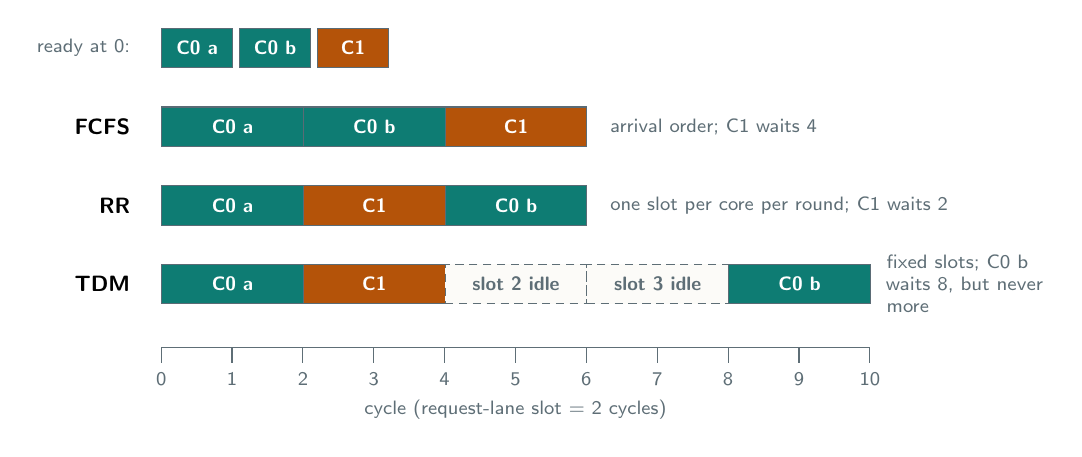
\begin{tikzpicture}[font=\sffamily\scriptsize, >=Latex, x=9mm, y=1mm]
  \tikzset{slot/.style={draw=octrule, minimum height=5mm, anchor=west, inner sep=0, font=\sffamily\scriptsize\bfseries, text=white},
           c0/.style={slot, fill=octteal}, c1/.style={slot, fill=octamber}, idle/.style={slot, fill=octpaper, text=octquiet, draw=octquiet, densely dashed},
           rowl/.style={anchor=east, font=\sffamily\footnotesize\bfseries}}
  % axis
  \foreach \t in {0,...,10} { \draw[octquiet] (\t, 2) -- (\t, 0); \node[below, text=octquiet] at (\t, 0) {\t}; }
  \draw[octquiet] (0, 2) -- (10, 2);
  \node[text=octquiet] at (5, -6) {cycle (request-lane slot = 2 cycles)};
  % ready marks
  \node[anchor=east, text=octquiet] at (-0.3, 40) {ready at 0:};
  \node[c0, minimum width=9mm] at (0, 40) {C0 a};
  \node[c0, minimum width=9mm] at (1.1, 40) {C0 b};
  \node[c1, minimum width=9mm] at (2.2, 40) {C1};
  % FCFS
  \node[rowl] at (-0.3, 30) {FCFS};
  \node[c0, minimum width=18mm] at (0, 30) {C0 a};
  \node[c0, minimum width=18mm] at (2, 30) {C0 b};
  \node[c1, minimum width=18mm] at (4, 30) {C1};
  \node[anchor=west, text=octquiet] at (6.2, 30) {arrival order; C1 waits 4};
  % RR
  \node[rowl] at (-0.3, 20) {RR};
  \node[c0, minimum width=18mm] at (0, 20) {C0 a};
  \node[c1, minimum width=18mm] at (2, 20) {C1};
  \node[c0, minimum width=18mm] at (4, 20) {C0 b};
  \node[anchor=west, text=octquiet] at (6.2, 20) {one slot per core per round; C1 waits 2};
  % TDM
  \node[rowl] at (-0.3, 10) {TDM};
  \node[c0, minimum width=18mm] at (0, 10) {C0 a};
  \node[c1, minimum width=18mm] at (2, 10) {C1};
  \node[idle, minimum width=18mm] at (4, 10) {slot 2 idle};
  \node[idle, minimum width=18mm] at (6, 10) {slot 3 idle};
  \node[c0, minimum width=18mm] at (8, 10) {C0 b};
  \node[anchor=west, text=octquiet, text width=20mm, align=left] at (10.1, 10) {fixed slots; C0 b waits 8, but never more};
\end{tikzpicture}
\end{adjustbox}
\caption{Three requests ready at the same cycle on one request lane --- two from core 0, one
from core 1 --- under the three shipped arbiters.}
\label{fig:arbitration}
\end{figure}

An arbiter is a subclass of \code{Arbiter} implementing one method:

\begin{lstlisting}[style=cpp]
virtual bool elect(uint64_t cycle_number,
                   vector<vector<Message> *> &buffers,   // one TX buffer per interface
                   Message *out_msg) = 0;                // the winner, if any
\end{lstlisting}

It is called once per interconnect tick for each lane that is free, with every interface's TX
buffer, and names the message that gets the lane (\cref{fig:arbitration}):

\begin{description}
\item[FCFS] (\code{FCFSArbiter}) picks the oldest message across all buffers: minimal average
  wait, no bound on how long a core may be starved by a busier one.
\item[Round-robin] (\code{RRArbiter}) rotates a pointer over the cores and grants the pointed
  core's oldest message if it has one, otherwise the next core that does: every core gets at
  most one slot per round, so a core's wait is bounded by one slot per competitor.
\item[TDM] (\code{TDMArbiter}) gives each core a fixed slot in a fixed cycle, whether or not it
  has anything to send; an owner with nothing ready leaves its slot idle. The wait is bounded by
  the period regardless of what other cores do --- the property real-time analyses want --- at
  the cost of throughput. It is the shipped default on \code{bus[0]}
  (\file{SplitBusController.csv}).
\end{description}

An arbiter that grants by owner takes the owner's \emph{oldest} message across all buffers,
not the first buffer in interface order that holds one: a core's cache-to-cache supplies sit in a
different buffer from its own requests and would otherwise be passed over round after round.
The helper is \code{electOldestOwned} in \code{Arbiter}; a new arbiter should use it too.

The arbiter of a bus is a configuration key, \key{arbiter\_type}, in the controller's CSV or
overridden per instance: \code{-p "bus[0].interconnect\_controller.arbiter\_type(s)=RRArbiter"}.
The LLC's data port has its own arbiter under the same interface, \key{llc\_controller.arbiter\_type}.
Adding an arbiter is a subclass, a line in \file{src/Arbiters/CMakeLists.txt} and a name in the
controller's factory (\cref{ch:extending}).

\section{Mesh and NoC}

\code{MultiCoreSystem\_Mesh.csv} replaces the bus with a \code{Mesh}: one node per entry of
\key{component\_ids}, and \key{connection\_matrix[i]} listing node $i$'s neighbours, the first
entry being the node itself. As shipped (\file{configuration/Interconnect/Mesh.csv}) the matrix
is the complete graph on the four L1s and the LLC (\cref{fig:topologies} middle), so every pair
has a direct link:

\begin{lstlisting}[style=csv]
component_ids(vi),0,1,2,3,10
connection_matrix[0](vi),0,1,2,3,10    # node 0 (L1 0) links to L1 1, L1 2, L1 3 and the LLC
connection_matrix[1](vi),1,0,2,3,10
connection_matrix[2](vi),2,0,1,3,10
connection_matrix[3](vi),3,0,1,2,10
connection_matrix[4](vi),10,0,1,2,3    # the LLC links to every L1
\end{lstlisting}

A different shape is a different matrix, no code: a ring is each node listing its two
neighbours. Each link each link carries requests and data on separate channels with
their own latencies (2 and 5 ticks) and its own arbiter (FCFS by default), half-duplex, one
message in flight per latency window. It is the natural home of the directory protocol, which
sends point-to-point and never broadcasts; directory MSI runs the whole EEMBC suite on it.

The \code{NoC} is the mesh plus \emph{switch} nodes (\key{switch\_ids}, 200 as shipped). A
switch is an interface that forwards whatever it receives in the same cycle, with no latency or
arbitration of its own, from a static per-source next-hop table built at construction: every
direct neighbour maps to itself, and everything a neighbouring switch lists maps to that
switch. As shipped (\cref{fig:topologies} right) the L1s link to the LLC directly and to each
other through the switch. A message can cross at most one switch, because a switch's own table
knows only its direct neighbours.

\begin{notebox}[What the NoC does not model yet]
Three things are worth knowing before measuring on it. A destination the routing table does not
know is dropped silently and \code{pushMessage} returns true; the TX-side capacity check
compares the \emph{number of per-link queues}, a constant, against the limit, so there is no
back-pressure on that side and congestion exits instead of stalling; and a hop is logged as one
opaque bus event, so the report's bus columns and the visualizer cannot see the path. A
multi-hop network with pluggable routing, per-hop credits and virtual networks per message
class remains future work; the current single-switch NoC is the supported implementation.
\end{notebox}

\begin{wherebox}
\begin{itemize}[nosep,leftmargin=1.2em]
\item \file{header/Interconnect/}, \file{src/Interconnect/} --- \code{Bus}, \code{TripleBus} and their interfaces
\item \file{src/Interconnect/BusController.cpp}, \file{src/Interconnect/SplitBusController.cpp}, \file{src/Interconnect/TripleBusController.cpp}, \file{src/Interconnect/UnifiedBusController.cpp}, \file{src/Interconnect/Point2PointController.cpp} --- the bus controllers
\item \file{src/Interconnect/Mesh.cpp}, \file{src/Interconnect/MeshController.cpp}, \file{src/Interconnect/NoC.cpp}, \file{src/Interconnect/NoCController.cpp} --- the mesh and the NoC
\item \file{header/Arbiters/}, \file{src/Arbiters/} --- \code{Arbiter}, \code{FCFSArbiter}, \code{RRArbiter}, \code{TDMArbiter}
\item \file{configuration/Interconnect/} --- latencies, buffer depths, arbiter names, the mesh and NoC connection matrices (\cref{app:config-keys})
\end{itemize}
\end{wherebox}

\chapter{Main memory}\label{ch:main-memory}

\whatyoufind{The two memory models behind \code{bus[1]}: a fixed-latency controller for fast
exploration and MCsim's cycle-accurate DDR4 controllers for fidelity; how each is selected,
clocked and stamped; the schedulers MCsim brings; and the two things that went wrong at this
boundary and are worth knowing.}

\section{Two models, one interface}

\begin{figure}[htbp]\centering
\begin{adjustbox}{max width=\textwidth}% The LLC, the memory bus and the two memory models, with their clocks.
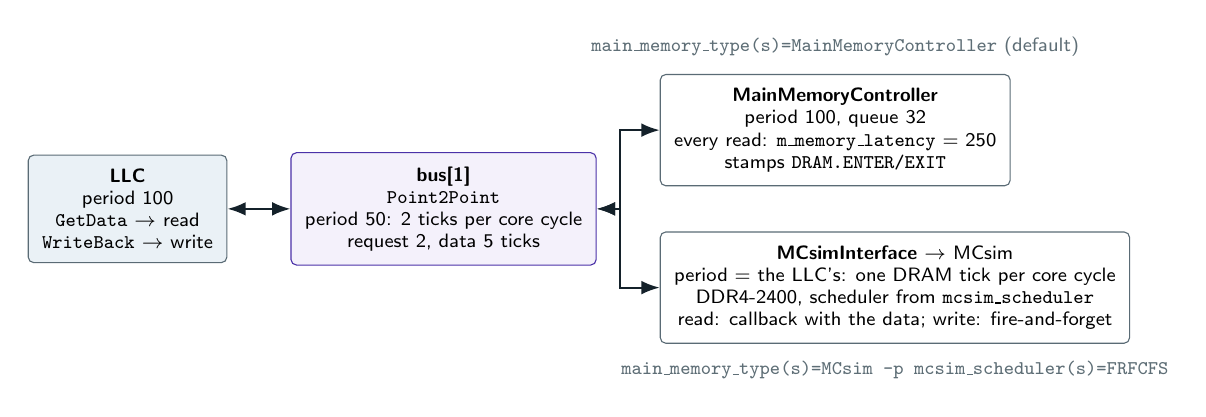
\begin{tikzpicture}[font=\sffamily\scriptsize, >=Latex, node distance=5mm and 8mm,
  b/.style={draw=octrule, fill=octmem, rounded corners=2pt, inner sep=5pt, align=center, minimum height=12mm},
  bus/.style={b, fill=octio, draw=octpurple},
  mem/.style={b, fill=white},
  w/.style={<->, thick, octink}, l/.style={font=\sffamily\scriptsize, text=octquiet, align=center}]
  \node[b] (llc) {\textbf{LLC}\\period 100\\\code{GetData} $\rightarrow$ read\\\code{WriteBack} $\rightarrow$ write};
  \node[bus, right=of llc] (bus) {\textbf{bus[1]}\\\code{Point2Point}\\period 50: 2 ticks per core cycle\\request 2, data 5 ticks};
  \node[mem, right=of bus, yshift=10mm] (fx) {\textbf{MainMemoryController}\\period 100, queue 32\\every read: \code{m\_memory\_latency} = 250\\stamps \code{DRAM.ENTER/EXIT}};
  \node[mem, right=of bus, yshift=-10mm] (mc) {\textbf{MCsimInterface} $\rightarrow$ MCsim\\period = the LLC's: one DRAM tick per core cycle\\DDR4-2400, scheduler from \code{mcsim\_scheduler}\\read: callback with the data; write: fire-and-forget};
  \draw[w] (llc) -- (bus);
  \draw[w] (bus.east) -- ++(3mm,0) |- (fx.west);
  \draw[w] (bus.east) -- ++(3mm,0) |- (mc.west);
  \node[l, above=1mm of fx] {\code{main\_memory\_type(s)=MainMemoryController} (default)};
  \node[l, below=1mm of mc] {\code{main\_memory\_type(s)=MCsim -p mcsim\_scheduler(s)=FRFCFS}};
\end{tikzpicture}
\end{adjustbox}
\caption{The LLC, the memory bus and the two memory models with their clocks.}
\label{fig:membus-mcsim}
\end{figure}

The LLC talks to memory through \code{bus[1]}, a point-to-point interconnect: a \act{GetData}
becomes a read, a \act{WriteBack} a write, and the fill comes back the same way
(\cref{fig:membus-mcsim}). Whatever answers on the far side is a \code{CommunicationInterface}
consumer, so the LLC does not know which model it is talking to; \key{main\_memory\_type}
selects it.

\paragraph{\code{MainMemoryController}} (the default) is a fixed-latency model: every read is
served \key{m\_memory\_latency} cycles after it is accepted (250 as shipped), from a queue of
\key{processing\_queue\_size} entries (32), at the cores' clock period. It stamps
\stamp{DRAM.ENTER} on acceptance and \stamp{DRAM.EXIT} when the data leaves, so the report's
\col{DRAM} column is exactly the service and \col{L2-DRAM Bus} the two bus legs
(\cref{ch:request-end-to-end}). It is the right model for design-space exploration where memory
is not the variable, and it is what the sweeps use as the baseline.

\paragraph{\code{MCsimInterface}} wraps MCsim, the extensible DRAM memory-controller simulator
vendored under \file{src/MCsim/}: a DDR4-2400 device with configurable channels, ranks, bank
groups and banks, per-requestor queues, and one scheduler chosen by \key{mcsim\_scheduler} from
the directories under \file{src/MCsim/system/}: FCFS, FR-FCFS (and its batched and capped
variants), BLISS, PAR-BS, MEDUSA, ORP, RTMem, ROC, RankReOrder, ReOrder, Round, PipeCAS, and the
predictable controllers AMC, DCmc, MAG, MCMC, PMC and RROF. Each is a \code{system.ini} that
names the request-queue structure, the command generator and the command scheduler; a new
controller is on average about 130 lines. MCsim stamps no DRAM events: the \col{DRAM} column
becomes the whole \code{bus[1]} round trip and \col{L2-DRAM Bus} the admit-to-leave hand-off.
Writes are fire-and-forget. Selecting it:

\begin{lstlisting}[style=shell]
-p "main_memory_type(s)=MCsim" -p "mcsim_scheduler(s)=FRFCFS"
\end{lstlisting}

MCsim is cycle-accurate and correspondingly slower --- five to ten times on EEMBC, and
prohibitive on the SPLASH giants, which is why the memory axis of the sweeps is EEMBC-only. Use
\code{FRFCFS} unless the scheduler is the subject: the \code{Round} and \code{ORP} schedulers
wedge on the shipped workloads.

\section{Clocks at the boundary}

The memory models are \code{ClockedObj}s like everything else, and both tick at the cores'
rate; what differs is what a tick means on the far side.

\begin{itemize}
\item \code{MainMemoryController} has no clock of its own to speak of: a read is served
  \key{m\_memory\_latency} core cycles after it is accepted. The DRAM is a delay, in core cycles.
\item \code{MCsimInterface} is constructed with the \emph{LLC's} period (one tick per core
  cycle) and tells MCsim that each tick is one cycle of a 2.4\,GHz core
  (\code{setCPUClockSpeed} in \file{src/MCsimInterface.cpp}). MCsim keeps its \emph{own} clock:
  its clock-domain crosser advances the DRAM by one command-clock cycle, $t_{CK}$ of the
  configured device (0.83\,ns for DDR4-2400), for every 0.42\,ns of core time, so the memory
  controller and the DRAM run at the device's real rate relative to the core and MCsim's timing
  parameters (\code{tRCD}, \code{tRP}, \code{tCL}, \ldots) stay in DRAM cycles. A request that
  spends $n$ DRAM cycles in MCsim therefore costs about $2n$ core cycles in the report.
\end{itemize}

The 2.4\,GHz figure is the one assumption at this boundary: the trace-driven core has no
frequency of its own, so the ratio between core and DRAM time is set here, in the bridge, and
is the same for every run.

The simulator is deterministic and its reports are byte-identical on Linux and Windows, MCsim
included; the environment check's reference run (\cref{ch:getting-started}) is an MCsim run for
that reason. \env{MCSIM\_PROBE} logs every request, command and completion with MCsim's own
clock when the DRAM model itself has to be examined (\cref{ch:monitoring}).

\begin{trapbox}[CRLF in the MCsim configuration]
MCsim's \code{.ini} parser rejects CRLF line endings with \emph{Malformed Line N (missing
equals)}. A tree checked out on Windows and copied to Linux has them; the environment check
tests for it.
\end{trapbox}

\begin{wherebox}
\begin{itemize}[nosep,leftmargin=1.2em]
\item \file{src/MainMemoryController.cpp}, \file{configuration/MainMemoryController.csv} --- the fixed-latency model
\item \file{header/MCsimInterface.h}, \file{src/MCsimInterface.cpp} --- the bridge to MCsim
\item \file{src/MCsim/} --- MCsim itself
\item \file{src/MCsim/README.md} --- writing a memory controller
\item \file{src/MCsim/system/<Name>/<Name>.ini} --- one per scheduler
\item \file{src/SystemConfigurations/MultiCoreSystem.cpp} --- where \key{main\_memory\_type} is read
\end{itemize}
\end{wherebox}

\chapter{Configuration}\label{ch:configuration}

\whatyoufind{To be written.}

\chapter{Monitoring: Logger, Debugger, trace and visualizer}\label{ch:monitoring}

\whatyoufind{To be written.}

\chapter{Periodic tasks and the interference demo}\label{ch:tasks-and-demo}

\whatyoufind{To be written.}

\chapter{Extending Octopus}\label{ch:extending}

\whatyoufind{To be written.}

\chapter{Integration modes: gem5 and the full-system stack}\label{ch:integration-modes}

\whatyoufind{To be written.}

\chapter{Evaluation}\label{ch:evaluation}

\whatyoufind{What the sweep harness measures and the figures this chapter will carry once the
sweeps have been re-run on the current code. The numbers themselves are deliberately absent:
the results and figures currently under \file{results/} were produced before the inclusive-LLC
eviction and bus-ordering fixes and are stale.}

\section{What is measured}

Every sweep script varies one axis against the fixed baseline --- snoop MESI, TripleBus, LRU,
FCFS bus, fixed-latency memory, default geometry --- over the EEMBC suite (and, for the
non-memory axes, SPLASH-2), and records per (value, benchmark) whether the run completed and the
worst case of every stage, the average effective latency, the finish cycle and the worst
head-of-queue latency (\cref{ch:configuration}, \cref{app:formats}). The per-axis component
shows \emph{where} a knob acts: the arbiter moves the bus columns, the LLC capacity the DRAM
column, the memory model the DRAM column again by a different amount, replacement almost
nothing.

\section{The figures to come}

\begin{itemize}
\item \textbf{Per-request worst-case latency by stage, across axes} --- the stacked bars that
  show which shared resource a knob moves (\code{fig1\_stage\_breakdown}).
\item \textbf{Mean versus worst-case latency by bus arbiter} --- FCFS, RR and TDM on a log
  scale: the predictability-for-throughput trade (\code{fig4\_wcet\_vs\_avg}).
\item \textbf{LLC capacity and the DRAM column} (\code{fig2\_cache\_capacity}); \textbf{fixed
  latency against MCsim} (\code{fig3\_memory\_dram}); \textbf{normalised latency across axes}
  (\code{fig5\_normalized}); \textbf{the axis-by-metric heatmap} (\code{fig6\_config\_heatmap});
  \textbf{completion status per configuration and benchmark} (\code{fig7\_status\_matrix}).
\item \textbf{The three acts of the demo} in numbers (\cref{tab:acts} already carries them).
\item \textbf{Analytical against measured}: the per-resource bound summed, against the measured
  worst case of the oldest request, which is the additive-latency argument of
  \cref{ch:introduction} made on this simulator.
\end{itemize}

\section{Reproducing}

\begin{lstlisting}[style=shell]
bash sweeps/sweep_all.sh                 # every single-axis sweep, EEMBC
bash sweeps/run_overnight.sh             # both suites, giants once under baseline
python sweeps/plot_results.py            # results/figures/*.{png,pdf}
\end{lstlisting}

\file{REPRODUCIBILITY.md} gives the runtime expectations per axis and suite and the artifact
map from figure to script; \file{results/README.md} explains the layout and the columns. When
the sweeps have been re-run, this chapter embeds the figures from \file{results/figures/} and
replaces this note.


\appendix
\chapter{Configuration key reference}\label{app:config-keys}

Every key in \file{configuration/**/*.csv} as shipped, one table per file, generated by
\file{docs/manual/tools/gen_config_tables.py} at build time. The type is the suffix the key
carries in the CSV (\code{(i)} integer, \code{(s)} string, \code{(vi)}/\code{(vs)} lists); the
value column is the shipped default. \Cref{ch:configuration} explains how files extend each
other and how a \code{-p} override reaches a key.

\footnotesize
% generated by tools/gen_config_tables.py -- do not edit

\subsection*{\texttt{configuration/SystemConfigurations/MultiCoreSystem.csv}}\label{cfg:configuration-systemconfigurations-multicoresystem-csv}
\begin{longtable}{@{}>{\ttfamily\raggedright\arraybackslash}p{0.33\textwidth}p{0.07\textwidth}>{\raggedright\arraybackslash}p{0.19\textwidth}>{\raggedright\arraybackslash}p{0.33\textwidth}@{}}
\toprule \normalfont key & type & value & meaning \\ \midrule \endfirsthead
\toprule \normalfont key & type & value & meaning \\ \midrule \endhead
\bottomrule \endfoot
workload\_\allowbreak{}path\index[cfg]{workload\_path@\code{workload\_path}} & string & \texttt{BMs/\allowbreak{}Test\allowbreak{}BM/\allowbreak{}} & Absolute path is recommended \\
num\_\allowbreak{}cores\index[cfg]{num\_cores@\code{num\_cores}} & int & \texttt{4} &  \\
bus\_\allowbreak{}type\index[cfg]{bus\_type@\code{bus\_type}} & string list & \texttt{Triple\allowbreak{}Bus,\allowbreak{} Bus} & Bus[0] (L1\textless{}-\textgreater{}LLC) is TripleBus: carries the LLC back-invalidation on its service channel. Bus[1] is LLC\textless{}-\textgreater{}memory \\
bus\allowbreak{}[0].\allowbreak{}controller\_\allowbreak{}type\index[cfg]{bus[0].controller\_type@\code{bus[0].controller\_type}} & string & \texttt{Split} & snoop broadcast bus \\
bus\allowbreak{}[0].\allowbreak{}interconnect\_\allowbreak{}controller.\allowbreak{}arbiter\_\allowbreak{}type\index[cfg]{bus[0].interconnect\_controller.arbiter\_type@\code{bus[0].interconnect\_controller.arbiter\_type}} & string & \texttt{FCFSArbiter} & Shared L1-LLC bus arbitration \\
bus\allowbreak{}[0].\allowbreak{}m\_\allowbreak{}lower\_\allowbreak{}level\_\allowbreak{}ids\index[cfg]{bus[0].m\_lower\_level\_ids@\code{bus[0].m\_lower\_level\_ids}} & int list & \texttt{0,\allowbreak{} 1,\allowbreak{} 2,\allowbreak{} 3} &  \\
bus\allowbreak{}[0].\allowbreak{}upper\_\allowbreak{}level\_\allowbreak{}cache\_\allowbreak{}ids\index[cfg]{bus[0].upper\_level\_cache\_ids@\code{bus[0].upper\_level\_cache\_ids}} & int list & \texttt{10} & LLC ID \\
bus\allowbreak{}[0].\allowbreak{}interconnect\_\allowbreak{}controller.\allowbreak{}wrr\_\allowbreak{}weight\index[cfg]{bus[0].interconnect\_controller.wrr\_weight@\code{bus[0].interconnect\_controller.wrr\_weight}} & int & \texttt{4} &  \\
cache\_\allowbreak{}controller\_\allowbreak{}type\index[cfg]{cache\_controller\_type@\code{cache\_controller\_type}} & string & \texttt{Cache\allowbreak{}Controller\allowbreak{}Exclusive} & L1 private caches: basic snoop controller \\
llc\_\allowbreak{}controller\_\allowbreak{}type\index[cfg]{llc\_controller\_type@\code{llc\_controller\_type}} & string & \texttt{Cache\allowbreak{}Controller\_\allowbreak{}End2End} & LLC: End2End controller drives TripleBus service channel for back-invalidation on eviction \\
bus\allowbreak{}[*].\allowbreak{}buffers\_\allowbreak{}max\_\allowbreak{}size\index[cfg]{bus[*].buffers\_max\_size@\code{bus[*].buffers\_max\_size}} & int & \texttt{256} & Response/request buffer depth: usable + in-flight reserve (sized to MSHR bound) \\
bus\allowbreak{}[0].\allowbreak{}response\_\allowbreak{}reserve\index[cfg]{bus[0].response\_reserve@\code{bus[0].response\_reserve}} & int & \texttt{128} & Snoop bus in-flight response reserve: request bus stalls when response buffer free space falls to this (bounds response-bus back-pressure without overflow or controller gating) \\
bus\allowbreak{}[1].\allowbreak{}m\_\allowbreak{}lower\_\allowbreak{}level\_\allowbreak{}ids\index[cfg]{bus[1].m\_lower\_level\_ids@\code{bus[1].m\_lower\_level\_ids}} & int list & \texttt{10} & LLC ID \\
bus\allowbreak{}[1].\allowbreak{}upper\_\allowbreak{}level\_\allowbreak{}cache\_\allowbreak{}ids\index[cfg]{bus[1].upper\_level\_cache\_ids@\code{bus[1].upper\_level\_cache\_ids}} & int list & \texttt{100} & Main memory ID \\
bus\allowbreak{}[1].\allowbreak{}controller\_\allowbreak{}type\index[cfg]{bus[1].controller\_type@\code{bus[1].controller\_type}} & string & \texttt{Point2Point} &  \\
bus\allowbreak{}[1].\allowbreak{}interconnect\_\allowbreak{}controller.\allowbreak{}candidates\_\allowbreak{}id\index[cfg]{bus[1].interconnect\_controller.candidates\_id@\code{bus[1].interconnect\_controller.candidates\_id}} & int list & \texttt{0,\allowbreak{} 1,\allowbreak{} 2,\allowbreak{} 3,\allowbreak{} 10} & Candidates are the l1 ids and llc id \\
cache\_\allowbreak{}controller\allowbreak{}[*].\allowbreak{}m\_\allowbreak{}shared\_\allowbreak{}memory\_\allowbreak{}id\index[cfg]{cache\_controller[*].m\_shared\_memory\_id@\code{cache\_controller[*].m\_shared\_memory\_id}} & int & \texttt{10} &  \\
cache\_\allowbreak{}controller\allowbreak{}[*].\allowbreak{}protocol\_\allowbreak{}type\index[cfg]{cache\_controller[*].protocol\_type@\code{cache\_controller[*].protocol\_type}} & string & \texttt{SNOOP\_\allowbreak{}MESI} &  \\
cache\_\allowbreak{}controller\allowbreak{}[*].\allowbreak{}fsm\_\allowbreak{}filename\index[cfg]{cache\_controller[*].fsm\_filename@\code{cache\_controller[*].fsm\_filename}} & string & \texttt{MESI\_\allowbreak{}split\allowbreak{}Bus\_\allowbreak{}snooping} &  \\
cache\_\allowbreak{}controller\allowbreak{}[*].\allowbreak{}num\_\allowbreak{}mshr\index[cfg]{cache\_controller[*].num\_mshr@\code{cache\_controller[*].num\_mshr}} & int & \texttt{16} & L1 MSHR depth (max concurrent outstanding misses). -1 = unbounded \\
cache\_\allowbreak{}controller\allowbreak{}[*].\allowbreak{}m\_\allowbreak{}data\_\allowbreak{}handler.\allowbreak{}pwb\_\allowbreak{}size\index[cfg]{cache\_controller[*].m\_data\_handler.pwb\_size@\code{cache\_controller[*].m\_data\_handler.pwb\_size}} & int & \texttt{8} & L1 write-back buffer depth. -1 = unbounded \\
cache\_\allowbreak{}controller\allowbreak{}[*].\allowbreak{}processing\_\allowbreak{}queue\_\allowbreak{}size\index[cfg]{cache\_controller[*].processing\_queue\_size@\code{cache\_controller[*].processing\_queue\_size}} & int & \texttt{16} & L1 processing-queue depth (bounds demand admission). -1 = unbounded \\
cache\_\allowbreak{}controller\allowbreak{}[0].\allowbreak{}m\_\allowbreak{}id\index[cfg]{cache\_controller[0].m\_id@\code{cache\_controller[0].m\_id}} & int & \texttt{0} &  \\
cache\_\allowbreak{}controller\allowbreak{}[1].\allowbreak{}m\_\allowbreak{}id\index[cfg]{cache\_controller[1].m\_id@\code{cache\_controller[1].m\_id}} & int & \texttt{1} &  \\
cache\_\allowbreak{}controller\allowbreak{}[2].\allowbreak{}m\_\allowbreak{}id\index[cfg]{cache\_controller[2].m\_id@\code{cache\_controller[2].m\_id}} & int & \texttt{2} &  \\
cache\_\allowbreak{}controller\allowbreak{}[3].\allowbreak{}m\_\allowbreak{}id\index[cfg]{cache\_controller[3].m\_id@\code{cache\_controller[3].m\_id}} & int & \texttt{3} &  \\
llc\_\allowbreak{}controller.\allowbreak{}m\_\allowbreak{}id\index[cfg]{llc\_controller.m\_id@\code{llc\_controller.m\_id}} & int & \texttt{10} & LLC \\
llc\_\allowbreak{}controller.\allowbreak{}m\_\allowbreak{}shared\_\allowbreak{}memory\_\allowbreak{}id\index[cfg]{llc\_controller.m\_shared\_memory\_id@\code{llc\_controller.m\_shared\_memory\_id}} & int & \texttt{100} & Id of the main memory \\
llc\_\allowbreak{}controller.\allowbreak{}protocol\_\allowbreak{}type\index[cfg]{llc\_controller.protocol\_type@\code{llc\_controller.protocol\_type}} & string & \texttt{SNOOP\_\allowbreak{}LLC\_\allowbreak{}MESI} &  \\
llc\_\allowbreak{}controller.\allowbreak{}fsm\_\allowbreak{}filename\index[cfg]{llc\_controller.fsm\_filename@\code{llc\_controller.fsm\_filename}} & string & \texttt{MESI\_\allowbreak{}LLC} &  \\
llc\_\allowbreak{}controller.\allowbreak{}m\_\allowbreak{}data\_\allowbreak{}handler.\allowbreak{}cache\_\allowbreak{}size\index[cfg]{llc\_controller.m\_data\_handler.cache\_size@\code{llc\_controller.m\_data\_handler.cache\_size}} & int & \texttt{32768} &  \\
llc\_\allowbreak{}controller.\allowbreak{}m\_\allowbreak{}data\_\allowbreak{}handler.\allowbreak{}m\_\allowbreak{}ways\_\allowbreak{}count\index[cfg]{llc\_controller.m\_data\_handler.m\_ways\_count@\code{llc\_controller.m\_data\_handler.m\_ways\_count}} & int & \texttt{2} &  \\
llc\_\allowbreak{}controller.\allowbreak{}m\_\allowbreak{}data\_\allowbreak{}handler.\allowbreak{}m\_\allowbreak{}data\_\allowbreak{}access\_\allowbreak{}latency\index[cfg]{llc\_controller.m\_data\_handler.m\_data\_access\_latency@\code{llc\_controller.m\_data\_handler.m\_data\_access\_latency}} & int & \texttt{10} &  \\
llc\_\allowbreak{}controller.\allowbreak{}num\_\allowbreak{}mshr\index[cfg]{llc\_controller.num\_mshr@\code{llc\_controller.num\_mshr}} & int & \texttt{64} & LLC MSHR depth: larger than L1 (fans in all cores). -1 = unbounded \\
llc\_\allowbreak{}controller.\allowbreak{}m\_\allowbreak{}data\_\allowbreak{}handler.\allowbreak{}pwb\_\allowbreak{}size\index[cfg]{llc\_controller.m\_data\_handler.pwb\_size@\code{llc\_controller.m\_data\_handler.pwb\_size}} & int & \texttt{32} & LLC write-back buffer depth: larger than L1. -1 = unbounded \\
llc\_\allowbreak{}controller.\allowbreak{}processing\_\allowbreak{}queue\_\allowbreak{}size\index[cfg]{llc\_controller.processing\_queue\_size@\code{llc\_controller.processing\_queue\_size}} & int & \texttt{64} & LLC processing-queue depth: larger than L1 (holds cache-to-cache forwarding concurrency). -1 = unbounded \\
llc\_\allowbreak{}controller.\allowbreak{}arbiter\_\allowbreak{}type\index[cfg]{llc\_controller.arbiter\_type@\code{llc\_controller.arbiter\_type}} & string & \texttt{FCFSArbiter} &  \\
llc\_\allowbreak{}controller.\allowbreak{}arbiter\_\allowbreak{}candidates\_\allowbreak{}ids\index[cfg]{llc\_controller.arbiter\_candidates\_ids@\code{llc\_controller.arbiter\_candidates\_ids}} & int list & \texttt{0,\allowbreak{} 1,\allowbreak{} 2,\allowbreak{} 3} & Candidates are the l1 ids \\
m\_\allowbreak{}main\_\allowbreak{}memory.\allowbreak{}m\_\allowbreak{}llc\_\allowbreak{}id\index[cfg]{m\_main\_memory.m\_llc\_id@\code{m\_main\_memory.m\_llc\_id}} & int & \texttt{10} &  \\
m\_\allowbreak{}main\_\allowbreak{}memory.\allowbreak{}m\_\allowbreak{}id\index[cfg]{m\_main\_memory.m\_id@\code{m\_main\_memory.m\_id}} & int & \texttt{100} &  \\
cache\_\allowbreak{}controller\allowbreak{}[*].\allowbreak{}dprint.\allowbreak{}enable\index[cfg]{cache\_controller[*].dprint.enable@\code{cache\_controller[*].dprint.enable}} & int & \texttt{0} &  \\
llc\_\allowbreak{}controller.\allowbreak{}dprint.\allowbreak{}enable\index[cfg]{llc\_controller.dprint.enable@\code{llc\_controller.dprint.enable}} & int & \texttt{0} &  \\
cache\_\allowbreak{}controller\allowbreak{}[*].\allowbreak{}dprint.\allowbreak{}target\index[cfg]{cache\_controller[*].dprint.target@\code{cache\_controller[*].dprint.target}} & string & \texttt{BMs/\allowbreak{}test\allowbreak{}DPrint/\allowbreak{}dprint.csv} &  \\
llc\_\allowbreak{}controller.\allowbreak{}dprint.\allowbreak{}target\index[cfg]{llc\_controller.dprint.target@\code{llc\_controller.dprint.target}} & string & \texttt{BMs/\allowbreak{}test\allowbreak{}DPrint/\allowbreak{}dprint.csv} &  \\
cache\_\allowbreak{}controller\allowbreak{}[*].\allowbreak{}dprint.\allowbreak{}addr\_\allowbreak{}filter\index[cfg]{cache\_controller[*].dprint.addr\_filter@\code{cache\_controller[*].dprint.addr\_filter}} & string & \texttt{} & filter in hexdecimal \\
llc\_\allowbreak{}controller.\allowbreak{}dprint.\allowbreak{}addr\_\allowbreak{}filter\index[cfg]{llc\_controller.dprint.addr\_filter@\code{llc\_controller.dprint.addr\_filter}} & string & \texttt{} & filter in hexdecimal \\
cache\_\allowbreak{}controller\allowbreak{}[*].\allowbreak{}dprint.\allowbreak{}cond\_\allowbreak{}addr\index[cfg]{cache\_controller[*].dprint.cond\_addr@\code{cache\_controller[*].dprint.cond\_addr}} & string list & \texttt{} & Acceptable Addresses \\
llc\_\allowbreak{}controller.\allowbreak{}dprint.\allowbreak{}cond\_\allowbreak{}addr\index[cfg]{llc\_controller.dprint.cond\_addr@\code{llc\_controller.dprint.cond\_addr}} & string list & \texttt{} & Acceptable Addresses \\
\end{longtable}

\subsection*{\texttt{configuration/SystemConfigurations/MultiCoreSystem\_Directory.csv}}\label{cfg:configuration-systemconfigurations-multicoresystem-directory-csv}
\begin{longtable}{@{}>{\ttfamily\raggedright\arraybackslash}p{0.33\textwidth}p{0.07\textwidth}>{\raggedright\arraybackslash}p{0.19\textwidth}>{\raggedright\arraybackslash}p{0.33\textwidth}@{}}
\toprule \normalfont key & type & value & meaning \\ \midrule \endfirsthead
\toprule \normalfont key & type & value & meaning \\ \midrule \endhead
\bottomrule \endfoot
workload\_\allowbreak{}path\index[cfg]{workload\_path@\code{workload\_path}} & string & \texttt{BMs/\allowbreak{}Test\allowbreak{}BM/\allowbreak{}} & Absolute path is recommended \\
num\_\allowbreak{}cores\index[cfg]{num\_cores@\code{num\_cores}} & int & \texttt{4} &  \\
bus\_\allowbreak{}type\index[cfg]{bus\_type@\code{bus\_type}} & string list & \texttt{Triple\allowbreak{}Bus,\allowbreak{} Bus} & Bus[0] is the interconnect between private caches and LLC and Bus[1] is between LLC and main memory \\
cache\_\allowbreak{}controller\_\allowbreak{}type\index[cfg]{cache\_controller\_type@\code{cache\_controller\_type}} & string & \texttt{Cache\allowbreak{}Controller\allowbreak{}Directory} & Type should match the name of the class \\
bus\allowbreak{}[*].\allowbreak{}buffers\_\allowbreak{}max\_\allowbreak{}size\index[cfg]{bus[*].buffers\_max\_size@\code{bus[*].buffers\_max\_size}} & int & \texttt{32} &  \\
bus\allowbreak{}[1].\allowbreak{}m\_\allowbreak{}lower\_\allowbreak{}level\_\allowbreak{}ids\index[cfg]{bus[1].m\_lower\_level\_ids@\code{bus[1].m\_lower\_level\_ids}} & int list & \texttt{10} & LLC ID \\
bus\allowbreak{}[1].\allowbreak{}upper\_\allowbreak{}level\_\allowbreak{}cache\_\allowbreak{}ids\index[cfg]{bus[1].upper\_level\_cache\_ids@\code{bus[1].upper\_level\_cache\_ids}} & int list & \texttt{100} & Main memory ID \\
bus\allowbreak{}[1].\allowbreak{}controller\_\allowbreak{}type\index[cfg]{bus[1].controller\_type@\code{bus[1].controller\_type}} & string & \texttt{Point2Point} &  \\
bus\allowbreak{}[1].\allowbreak{}interconnect\_\allowbreak{}controller.\allowbreak{}candidates\_\allowbreak{}id\index[cfg]{bus[1].interconnect\_controller.candidates\_id@\code{bus[1].interconnect\_controller.candidates\_id}} & int list & \texttt{0,\allowbreak{} 1,\allowbreak{} 2,\allowbreak{} 3,\allowbreak{} 10} & Candidates are the l1 ids and llc id \\
bus\allowbreak{}[0].\allowbreak{}interconnect\_\allowbreak{}controller.\allowbreak{}arbiter\_\allowbreak{}type\index[cfg]{bus[0].interconnect\_controller.arbiter\_type@\code{bus[0].interconnect\_controller.arbiter\_type}} & string & \texttt{FCFSArbiter} & Pinned: every directory validation was done under FCFS. The shared SplitBusController default is TDM (for snoop) and directory+TDM starves one core on aifirf01/cacheb01 -- an open bug rather than a config choice \\
cache\_\allowbreak{}controller\allowbreak{}[*].\allowbreak{}m\_\allowbreak{}shared\_\allowbreak{}memory\_\allowbreak{}id\index[cfg]{cache\_controller[*].m\_shared\_memory\_id@\code{cache\_controller[*].m\_shared\_memory\_id}} & int & \texttt{10} &  \\
cache\_\allowbreak{}controller\allowbreak{}[*].\allowbreak{}protocol\_\allowbreak{}type\index[cfg]{cache\_controller[*].protocol\_type@\code{cache\_controller[*].protocol\_type}} & string & \texttt{DIRECTORY\_\allowbreak{}MSI} &  \\
cache\_\allowbreak{}controller\allowbreak{}[*].\allowbreak{}fsm\_\allowbreak{}filename\index[cfg]{cache\_controller[*].fsm\_filename@\code{cache\_controller[*].fsm\_filename}} & string & \texttt{MSI\_\allowbreak{}directory} &  \\
cache\_\allowbreak{}controller\allowbreak{}[*].\allowbreak{}num\_\allowbreak{}mshr\index[cfg]{cache\_controller[*].num\_mshr@\code{cache\_controller[*].num\_mshr}} & int & \texttt{16} & L1 MSHR depth (max concurrent outstanding misses). -1 = unbounded \\
cache\_\allowbreak{}controller\allowbreak{}[*].\allowbreak{}m\_\allowbreak{}data\_\allowbreak{}handler.\allowbreak{}pwb\_\allowbreak{}size\index[cfg]{cache\_controller[*].m\_data\_handler.pwb\_size@\code{cache\_controller[*].m\_data\_handler.pwb\_size}} & int & \texttt{8} & L1 write-back buffer depth. -1 = unbounded \\
cache\_\allowbreak{}controller\allowbreak{}[*].\allowbreak{}processing\_\allowbreak{}queue\_\allowbreak{}size\index[cfg]{cache\_controller[*].processing\_queue\_size@\code{cache\_controller[*].processing\_queue\_size}} & int & \texttt{16} & L1 processing-queue depth (bounds demand admission). -1 = unbounded \\
cache\_\allowbreak{}controller\allowbreak{}[0].\allowbreak{}m\_\allowbreak{}id\index[cfg]{cache\_controller[0].m\_id@\code{cache\_controller[0].m\_id}} & int & \texttt{0} &  \\
cache\_\allowbreak{}controller\allowbreak{}[1].\allowbreak{}m\_\allowbreak{}id\index[cfg]{cache\_controller[1].m\_id@\code{cache\_controller[1].m\_id}} & int & \texttt{1} &  \\
cache\_\allowbreak{}controller\allowbreak{}[2].\allowbreak{}m\_\allowbreak{}id\index[cfg]{cache\_controller[2].m\_id@\code{cache\_controller[2].m\_id}} & int & \texttt{2} &  \\
cache\_\allowbreak{}controller\allowbreak{}[3].\allowbreak{}m\_\allowbreak{}id\index[cfg]{cache\_controller[3].m\_id@\code{cache\_controller[3].m\_id}} & int & \texttt{3} &  \\
llc\_\allowbreak{}controller.\allowbreak{}m\_\allowbreak{}id\index[cfg]{llc\_controller.m\_id@\code{llc\_controller.m\_id}} & int & \texttt{10} & LLC \\
llc\_\allowbreak{}controller.\allowbreak{}m\_\allowbreak{}shared\_\allowbreak{}memory\_\allowbreak{}id\index[cfg]{llc\_controller.m\_shared\_memory\_id@\code{llc\_controller.m\_shared\_memory\_id}} & int & \texttt{100} & Id of the main memory \\
llc\_\allowbreak{}controller.\allowbreak{}protocol\_\allowbreak{}type\index[cfg]{llc\_controller.protocol\_type@\code{llc\_controller.protocol\_type}} & string & \texttt{DIRECTORY\_\allowbreak{}LLC\_\allowbreak{}MSI} &  \\
llc\_\allowbreak{}controller.\allowbreak{}fsm\_\allowbreak{}filename\index[cfg]{llc\_controller.fsm\_filename@\code{llc\_controller.fsm\_filename}} & string & \texttt{MSI\_\allowbreak{}LLC\_\allowbreak{}directory} &  \\
llc\_\allowbreak{}controller.\allowbreak{}m\_\allowbreak{}data\_\allowbreak{}handler.\allowbreak{}cache\_\allowbreak{}size\index[cfg]{llc\_controller.m\_data\_handler.cache\_size@\code{llc\_controller.m\_data\_handler.cache\_size}} & int & \texttt{32768} &  \\
llc\_\allowbreak{}controller.\allowbreak{}m\_\allowbreak{}data\_\allowbreak{}handler.\allowbreak{}m\_\allowbreak{}ways\_\allowbreak{}count\index[cfg]{llc\_controller.m\_data\_handler.m\_ways\_count@\code{llc\_controller.m\_data\_handler.m\_ways\_count}} & int & \texttt{2} &  \\
llc\_\allowbreak{}controller.\allowbreak{}m\_\allowbreak{}data\_\allowbreak{}handler.\allowbreak{}m\_\allowbreak{}data\_\allowbreak{}access\_\allowbreak{}latency\index[cfg]{llc\_controller.m\_data\_handler.m\_data\_access\_latency@\code{llc\_controller.m\_data\_handler.m\_data\_access\_latency}} & int & \texttt{10} &  \\
llc\_\allowbreak{}controller.\allowbreak{}num\_\allowbreak{}mshr\index[cfg]{llc\_controller.num\_mshr@\code{llc\_controller.num\_mshr}} & int & \texttt{64} & LLC MSHR depth: larger than L1 (fans in all cores). -1 = unbounded \\
llc\_\allowbreak{}controller.\allowbreak{}m\_\allowbreak{}data\_\allowbreak{}handler.\allowbreak{}pwb\_\allowbreak{}size\index[cfg]{llc\_controller.m\_data\_handler.pwb\_size@\code{llc\_controller.m\_data\_handler.pwb\_size}} & int & \texttt{32} & LLC write-back buffer depth: larger than L1. -1 = unbounded \\
llc\_\allowbreak{}controller.\allowbreak{}processing\_\allowbreak{}queue\_\allowbreak{}size\index[cfg]{llc\_controller.processing\_queue\_size@\code{llc\_controller.processing\_queue\_size}} & int & \texttt{32} & LLC processing-queue depth: larger than L1. -1 = unbounded \\
llc\_\allowbreak{}controller.\allowbreak{}arbiter\_\allowbreak{}type\index[cfg]{llc\_controller.arbiter\_type@\code{llc\_controller.arbiter\_type}} & string & \texttt{FCFSArbiter} &  \\
llc\_\allowbreak{}controller.\allowbreak{}arbiter\_\allowbreak{}candidates\_\allowbreak{}ids\index[cfg]{llc\_controller.arbiter\_candidates\_ids@\code{llc\_controller.arbiter\_candidates\_ids}} & int list & \texttt{0,\allowbreak{} 1,\allowbreak{} 2,\allowbreak{} 3} & Candidates are the l1 ids \\
m\_\allowbreak{}main\_\allowbreak{}memory.\allowbreak{}m\_\allowbreak{}llc\_\allowbreak{}id\index[cfg]{m\_main\_memory.m\_llc\_id@\code{m\_main\_memory.m\_llc\_id}} & int & \texttt{10} &  \\
m\_\allowbreak{}main\_\allowbreak{}memory.\allowbreak{}m\_\allowbreak{}id\index[cfg]{m\_main\_memory.m\_id@\code{m\_main\_memory.m\_id}} & int & \texttt{100} &  \\
cache\_\allowbreak{}controller\allowbreak{}[*].\allowbreak{}dprint.\allowbreak{}enable\index[cfg]{cache\_controller[*].dprint.enable@\code{cache\_controller[*].dprint.enable}} & int & \texttt{0} &  \\
llc\_\allowbreak{}controller.\allowbreak{}dprint.\allowbreak{}enable\index[cfg]{llc\_controller.dprint.enable@\code{llc\_controller.dprint.enable}} & int & \texttt{0} &  \\
cache\_\allowbreak{}controller\allowbreak{}[*].\allowbreak{}dprint.\allowbreak{}target\index[cfg]{cache\_controller[*].dprint.target@\code{cache\_controller[*].dprint.target}} & string & \texttt{BMs/\allowbreak{}test\allowbreak{}DPrint/\allowbreak{}dprint.csv} &  \\
llc\_\allowbreak{}controller.\allowbreak{}dprint.\allowbreak{}target\index[cfg]{llc\_controller.dprint.target@\code{llc\_controller.dprint.target}} & string & \texttt{BMs/\allowbreak{}test\allowbreak{}DPrint/\allowbreak{}dprint.csv} &  \\
cache\_\allowbreak{}controller\allowbreak{}[*].\allowbreak{}dprint.\allowbreak{}addr\_\allowbreak{}filter\index[cfg]{cache\_controller[*].dprint.addr\_filter@\code{cache\_controller[*].dprint.addr\_filter}} & string & \texttt{} & filter in hexdecimal \\
llc\_\allowbreak{}controller.\allowbreak{}dprint.\allowbreak{}addr\_\allowbreak{}filter\index[cfg]{llc\_controller.dprint.addr\_filter@\code{llc\_controller.dprint.addr\_filter}} & string & \texttt{} & filter in hexdecimal \\
cache\_\allowbreak{}controller\allowbreak{}[*].\allowbreak{}dprint.\allowbreak{}cond\_\allowbreak{}addr\index[cfg]{cache\_controller[*].dprint.cond\_addr@\code{cache\_controller[*].dprint.cond\_addr}} & string list & \texttt{} & Acceptable Addresses \\
llc\_\allowbreak{}controller.\allowbreak{}dprint.\allowbreak{}cond\_\allowbreak{}addr\index[cfg]{llc\_controller.dprint.cond\_addr@\code{llc\_controller.dprint.cond\_addr}} & string list & \texttt{} & Acceptable Addresses \\
\end{longtable}

\subsection*{\texttt{configuration/SystemConfigurations/MultiCoreSystem\_Mesh.csv}}\label{cfg:configuration-systemconfigurations-multicoresystem-mesh-csv}
\begin{longtable}{@{}>{\ttfamily\raggedright\arraybackslash}p{0.33\textwidth}p{0.07\textwidth}>{\raggedright\arraybackslash}p{0.19\textwidth}>{\raggedright\arraybackslash}p{0.33\textwidth}@{}}
\toprule \normalfont key & type & value & meaning \\ \midrule \endfirsthead
\toprule \normalfont key & type & value & meaning \\ \midrule \endhead
\bottomrule \endfoot
workload\_\allowbreak{}path\index[cfg]{workload\_path@\code{workload\_path}} & string & \texttt{BMs/\allowbreak{}Test\allowbreak{}BM/\allowbreak{}} & Absolute path is recommended \\
num\_\allowbreak{}cores\index[cfg]{num\_cores@\code{num\_cores}} & int & \texttt{4} &  \\
cache\_\allowbreak{}controller\_\allowbreak{}type\index[cfg]{cache\_controller\_type@\code{cache\_controller\_type}} & string & \texttt{Cache\allowbreak{}Controller\allowbreak{}Directory} & Type should match the name of the class \\
interconnect\_\allowbreak{}type\index[cfg]{interconnect\_type@\code{interconnect\_type}} & string & \texttt{No\allowbreak{}C} &  \\
interconnect.\allowbreak{}buffers\_\allowbreak{}max\_\allowbreak{}size\index[cfg]{interconnect.buffers\_max\_size@\code{interconnect.buffers\_max\_size}} & int & \texttt{32} &  \\
bus.\allowbreak{}buffers\_\allowbreak{}max\_\allowbreak{}size\index[cfg]{bus.buffers\_max\_size@\code{bus.buffers\_max\_size}} & int & \texttt{32} &  \\
bus.\allowbreak{}m\_\allowbreak{}lower\_\allowbreak{}level\_\allowbreak{}ids\index[cfg]{bus.m\_lower\_level\_ids@\code{bus.m\_lower\_level\_ids}} & int list & \texttt{10} & LLC ID \\
bus.\allowbreak{}upper\_\allowbreak{}level\_\allowbreak{}cache\_\allowbreak{}ids\index[cfg]{bus.upper\_level\_cache\_ids@\code{bus.upper\_level\_cache\_ids}} & int list & \texttt{100} & Main memory ID \\
bus.\allowbreak{}controller\_\allowbreak{}type\index[cfg]{bus.controller\_type@\code{bus.controller\_type}} & string & \texttt{Point2Point} &  \\
bus.\allowbreak{}interconnect\_\allowbreak{}controller.\allowbreak{}candidates\_\allowbreak{}id\index[cfg]{bus.interconnect\_controller.candidates\_id@\code{bus.interconnect\_controller.candidates\_id}} & int list & \texttt{0,\allowbreak{} 1,\allowbreak{} 2,\allowbreak{} 3,\allowbreak{} 10} & Candidates are the l1 ids and llc id \\
cache\_\allowbreak{}controller\allowbreak{}[*].\allowbreak{}m\_\allowbreak{}shared\_\allowbreak{}memory\_\allowbreak{}id\index[cfg]{cache\_controller[*].m\_shared\_memory\_id@\code{cache\_controller[*].m\_shared\_memory\_id}} & int & \texttt{10} &  \\
cache\_\allowbreak{}controller\allowbreak{}[*].\allowbreak{}protocol\_\allowbreak{}type\index[cfg]{cache\_controller[*].protocol\_type@\code{cache\_controller[*].protocol\_type}} & string & \texttt{DIRECTORY\_\allowbreak{}MSI} &  \\
cache\_\allowbreak{}controller\allowbreak{}[*].\allowbreak{}fsm\_\allowbreak{}filename\index[cfg]{cache\_controller[*].fsm\_filename@\code{cache\_controller[*].fsm\_filename}} & string & \texttt{MSI\_\allowbreak{}directory} &  \\
cache\_\allowbreak{}controller\allowbreak{}[*].\allowbreak{}processing\_\allowbreak{}queue\_\allowbreak{}size\index[cfg]{cache\_controller[*].processing\_queue\_size@\code{cache\_controller[*].processing\_queue\_size}} & int & \texttt{16} & L1 processing-queue depth (bounds demand admission). -1 = unbounded \\
cache\_\allowbreak{}controller\allowbreak{}[0].\allowbreak{}m\_\allowbreak{}id\index[cfg]{cache\_controller[0].m\_id@\code{cache\_controller[0].m\_id}} & int & \texttt{0} &  \\
cache\_\allowbreak{}controller\allowbreak{}[1].\allowbreak{}m\_\allowbreak{}id\index[cfg]{cache\_controller[1].m\_id@\code{cache\_controller[1].m\_id}} & int & \texttt{1} &  \\
cache\_\allowbreak{}controller\allowbreak{}[2].\allowbreak{}m\_\allowbreak{}id\index[cfg]{cache\_controller[2].m\_id@\code{cache\_controller[2].m\_id}} & int & \texttt{2} &  \\
cache\_\allowbreak{}controller\allowbreak{}[3].\allowbreak{}m\_\allowbreak{}id\index[cfg]{cache\_controller[3].m\_id@\code{cache\_controller[3].m\_id}} & int & \texttt{3} &  \\
llc\_\allowbreak{}controller.\allowbreak{}m\_\allowbreak{}id\index[cfg]{llc\_controller.m\_id@\code{llc\_controller.m\_id}} & int & \texttt{10} & LLC \\
llc\_\allowbreak{}controller.\allowbreak{}m\_\allowbreak{}shared\_\allowbreak{}memory\_\allowbreak{}id\index[cfg]{llc\_controller.m\_shared\_memory\_id@\code{llc\_controller.m\_shared\_memory\_id}} & int & \texttt{100} & Id of the main memory \\
llc\_\allowbreak{}controller.\allowbreak{}protocol\_\allowbreak{}type\index[cfg]{llc\_controller.protocol\_type@\code{llc\_controller.protocol\_type}} & string & \texttt{DIRECTORY\_\allowbreak{}LLC\_\allowbreak{}MSI} &  \\
llc\_\allowbreak{}controller.\allowbreak{}fsm\_\allowbreak{}filename\index[cfg]{llc\_controller.fsm\_filename@\code{llc\_controller.fsm\_filename}} & string & \texttt{MSI\_\allowbreak{}LLC\_\allowbreak{}directory} &  \\
llc\_\allowbreak{}controller.\allowbreak{}num\_\allowbreak{}mshr\index[cfg]{llc\_controller.num\_mshr@\code{llc\_controller.num\_mshr}} & int & \texttt{64} & LLC MSHR depth: larger than L1 (fans in all cores). -1 = unbounded \\
llc\_\allowbreak{}controller.\allowbreak{}m\_\allowbreak{}data\_\allowbreak{}handler.\allowbreak{}pwb\_\allowbreak{}size\index[cfg]{llc\_controller.m\_data\_handler.pwb\_size@\code{llc\_controller.m\_data\_handler.pwb\_size}} & int & \texttt{32} & LLC write-back buffer depth: larger than L1. -1 = unbounded \\
llc\_\allowbreak{}controller.\allowbreak{}processing\_\allowbreak{}queue\_\allowbreak{}size\index[cfg]{llc\_controller.processing\_queue\_size@\code{llc\_controller.processing\_queue\_size}} & int & \texttt{32} & LLC processing-queue depth: larger than L1. -1 = unbounded \\
llc\_\allowbreak{}controller.\allowbreak{}m\_\allowbreak{}data\_\allowbreak{}handler.\allowbreak{}cache\_\allowbreak{}size\index[cfg]{llc\_controller.m\_data\_handler.cache\_size@\code{llc\_controller.m\_data\_handler.cache\_size}} & int & \texttt{32768} &  \\
llc\_\allowbreak{}controller.\allowbreak{}m\_\allowbreak{}data\_\allowbreak{}handler.\allowbreak{}m\_\allowbreak{}ways\_\allowbreak{}count\index[cfg]{llc\_controller.m\_data\_handler.m\_ways\_count@\code{llc\_controller.m\_data\_handler.m\_ways\_count}} & int & \texttt{2} &  \\
llc\_\allowbreak{}controller.\allowbreak{}m\_\allowbreak{}data\_\allowbreak{}handler.\allowbreak{}m\_\allowbreak{}data\_\allowbreak{}access\_\allowbreak{}latency\index[cfg]{llc\_controller.m\_data\_handler.m\_data\_access\_latency@\code{llc\_controller.m\_data\_handler.m\_data\_access\_latency}} & int & \texttt{10} &  \\
llc\_\allowbreak{}controller.\allowbreak{}arbiter\_\allowbreak{}type\index[cfg]{llc\_controller.arbiter\_type@\code{llc\_controller.arbiter\_type}} & string & \texttt{FCFSArbiter} &  \\
llc\_\allowbreak{}controller.\allowbreak{}arbiter\_\allowbreak{}candidates\_\allowbreak{}ids\index[cfg]{llc\_controller.arbiter\_candidates\_ids@\code{llc\_controller.arbiter\_candidates\_ids}} & int list & \texttt{0,\allowbreak{} 1,\allowbreak{} 2,\allowbreak{} 3} & Candidates are the l1 ids \\
m\_\allowbreak{}main\_\allowbreak{}memory.\allowbreak{}m\_\allowbreak{}llc\_\allowbreak{}id\index[cfg]{m\_main\_memory.m\_llc\_id@\code{m\_main\_memory.m\_llc\_id}} & int & \texttt{10} &  \\
m\_\allowbreak{}main\_\allowbreak{}memory.\allowbreak{}m\_\allowbreak{}id\index[cfg]{m\_main\_memory.m\_id@\code{m\_main\_memory.m\_id}} & int & \texttt{100} &  \\
cache\_\allowbreak{}controller\allowbreak{}[2].\allowbreak{}dprint.\allowbreak{}enable\index[cfg]{cache\_controller[2].dprint.enable@\code{cache\_controller[2].dprint.enable}} & int & \texttt{0} &  \\
llc\_\allowbreak{}controller.\allowbreak{}dprint.\allowbreak{}enable\index[cfg]{llc\_controller.dprint.enable@\code{llc\_controller.dprint.enable}} & int & \texttt{0} &  \\
cache\_\allowbreak{}controller\allowbreak{}[*].\allowbreak{}dprint.\allowbreak{}target\index[cfg]{cache\_controller[*].dprint.target@\code{cache\_controller[*].dprint.target}} & string & \texttt{} &  \\
llc\_\allowbreak{}controller.\allowbreak{}dprint.\allowbreak{}target\index[cfg]{llc\_controller.dprint.target@\code{llc\_controller.dprint.target}} & string & \texttt{BMs/\allowbreak{}test\allowbreak{}DPrint/\allowbreak{}dprint.csv} &  \\
cache\_\allowbreak{}controller\allowbreak{}[*].\allowbreak{}dprint.\allowbreak{}addr\_\allowbreak{}filter\index[cfg]{cache\_controller[*].dprint.addr\_filter@\code{cache\_controller[*].dprint.addr\_filter}} & string & \texttt{0x\allowbreak{}FFFFFFFF\allowbreak{}FFFFFFC0} & filter in hexdecimal \\
llc\_\allowbreak{}controller.\allowbreak{}dprint.\allowbreak{}addr\_\allowbreak{}filter\index[cfg]{llc\_controller.dprint.addr\_filter@\code{llc\_controller.dprint.addr\_filter}} & string & \texttt{0x\allowbreak{}FFFFFFFF\allowbreak{}FFFFFFC0} & filter in hexdecimal \\
cache\_\allowbreak{}controller\allowbreak{}[*].\allowbreak{}dprint.\allowbreak{}cond\_\allowbreak{}addr\index[cfg]{cache\_controller[*].dprint.cond\_addr@\code{cache\_controller[*].dprint.cond\_addr}} & string list & \texttt{} & Acceptable Addresses \\
llc\_\allowbreak{}controller.\allowbreak{}dprint.\allowbreak{}cond\_\allowbreak{}addr\index[cfg]{llc\_controller.dprint.cond\_addr@\code{llc\_controller.dprint.cond\_addr}} & string list & \texttt{} & Acceptable Addresses \\
cache\_\allowbreak{}controller\allowbreak{}[2].\allowbreak{}dprint.\allowbreak{}cond\_\allowbreak{}msg\_\allowbreak{}id\index[cfg]{cache\_controller[2].dprint.cond\_msg\_id@\code{cache\_controller[2].dprint.cond\_msg\_id}} & int list & \texttt{245788} &  \\
\end{longtable}

\subsection*{\texttt{configuration/SystemConfigurations/MultiCoreSystem\_Snoop.csv}}\label{cfg:configuration-systemconfigurations-multicoresystem-snoop-csv}
\begin{longtable}{@{}>{\ttfamily\raggedright\arraybackslash}p{0.33\textwidth}p{0.07\textwidth}>{\raggedright\arraybackslash}p{0.19\textwidth}>{\raggedright\arraybackslash}p{0.33\textwidth}@{}}
\toprule \normalfont key & type & value & meaning \\ \midrule \endfirsthead
\toprule \normalfont key & type & value & meaning \\ \midrule \endhead
\bottomrule \endfoot
workload\_\allowbreak{}path\index[cfg]{workload\_path@\code{workload\_path}} & string & \texttt{BMs/\allowbreak{}Test\allowbreak{}BM/\allowbreak{}} & Absolute path is recommended \\
num\_\allowbreak{}cores\index[cfg]{num\_cores@\code{num\_cores}} & int & \texttt{4} &  \\
bus\_\allowbreak{}type\index[cfg]{bus\_type@\code{bus\_type}} & string list & \texttt{Triple\allowbreak{}Bus,\allowbreak{} Bus} & Bus[0] (L1\textless{}-\textgreater{}LLC) is TripleBus: carries the LLC back-invalidation on its service channel. Bus[1] is LLC\textless{}-\textgreater{}memory \\
bus\allowbreak{}[0].\allowbreak{}controller\_\allowbreak{}type\index[cfg]{bus[0].controller\_type@\code{bus[0].controller\_type}} & string & \texttt{Split} & snoop broadcast bus \\
bus\allowbreak{}[0].\allowbreak{}interconnect\_\allowbreak{}controller.\allowbreak{}arbiter\_\allowbreak{}type\index[cfg]{bus[0].interconnect\_controller.arbiter\_type@\code{bus[0].interconnect\_controller.arbiter\_type}} & string & \texttt{FCFSArbiter} & Shared L1-LLC bus arbitration \\
bus\allowbreak{}[0].\allowbreak{}m\_\allowbreak{}lower\_\allowbreak{}level\_\allowbreak{}ids\index[cfg]{bus[0].m\_lower\_level\_ids@\code{bus[0].m\_lower\_level\_ids}} & int list & \texttt{0,\allowbreak{} 1,\allowbreak{} 2,\allowbreak{} 3} &  \\
bus\allowbreak{}[0].\allowbreak{}upper\_\allowbreak{}level\_\allowbreak{}cache\_\allowbreak{}ids\index[cfg]{bus[0].upper\_level\_cache\_ids@\code{bus[0].upper\_level\_cache\_ids}} & int list & \texttt{10} & LLC ID \\
cache\_\allowbreak{}controller\_\allowbreak{}type\index[cfg]{cache\_controller\_type@\code{cache\_controller\_type}} & string & \texttt{Cache\allowbreak{}Controller} & L1 private caches: basic snoop controller \\
llc\_\allowbreak{}controller\_\allowbreak{}type\index[cfg]{llc\_controller\_type@\code{llc\_controller\_type}} & string & \texttt{Cache\allowbreak{}Controller\_\allowbreak{}End2End} & LLC: End2End controller drives TripleBus service channel for back-invalidation on eviction \\
bus\allowbreak{}[*].\allowbreak{}buffers\_\allowbreak{}max\_\allowbreak{}size\index[cfg]{bus[*].buffers\_max\_size@\code{bus[*].buffers\_max\_size}} & int & \texttt{256} & Response/request buffer depth: usable + in-flight reserve (sized to MSHR bound) \\
bus\allowbreak{}[0].\allowbreak{}response\_\allowbreak{}reserve\index[cfg]{bus[0].response\_reserve@\code{bus[0].response\_reserve}} & int & \texttt{128} & Snoop bus in-flight response reserve: request bus stalls when response buffer free space falls to this (bounds response-bus back-pressure without overflow or controller gating) \\
bus\allowbreak{}[1].\allowbreak{}m\_\allowbreak{}lower\_\allowbreak{}level\_\allowbreak{}ids\index[cfg]{bus[1].m\_lower\_level\_ids@\code{bus[1].m\_lower\_level\_ids}} & int list & \texttt{10} & LLC ID \\
bus\allowbreak{}[1].\allowbreak{}upper\_\allowbreak{}level\_\allowbreak{}cache\_\allowbreak{}ids\index[cfg]{bus[1].upper\_level\_cache\_ids@\code{bus[1].upper\_level\_cache\_ids}} & int list & \texttt{100} & Main memory ID \\
bus\allowbreak{}[1].\allowbreak{}controller\_\allowbreak{}type\index[cfg]{bus[1].controller\_type@\code{bus[1].controller\_type}} & string & \texttt{Point2Point} &  \\
bus\allowbreak{}[1].\allowbreak{}interconnect\_\allowbreak{}controller.\allowbreak{}candidates\_\allowbreak{}id\index[cfg]{bus[1].interconnect\_controller.candidates\_id@\code{bus[1].interconnect\_controller.candidates\_id}} & int list & \texttt{0,\allowbreak{} 1,\allowbreak{} 2,\allowbreak{} 3,\allowbreak{} 10} & Candidates are the l1 ids and llc id \\
cache\_\allowbreak{}controller\allowbreak{}[*].\allowbreak{}m\_\allowbreak{}shared\_\allowbreak{}memory\_\allowbreak{}id\index[cfg]{cache\_controller[*].m\_shared\_memory\_id@\code{cache\_controller[*].m\_shared\_memory\_id}} & int & \texttt{10} &  \\
cache\_\allowbreak{}controller\allowbreak{}[*].\allowbreak{}protocol\_\allowbreak{}type\index[cfg]{cache\_controller[*].protocol\_type@\code{cache\_controller[*].protocol\_type}} & string & \texttt{SNOOP\_\allowbreak{}MSI} &  \\
cache\_\allowbreak{}controller\allowbreak{}[*].\allowbreak{}fsm\_\allowbreak{}filename\index[cfg]{cache\_controller[*].fsm\_filename@\code{cache\_controller[*].fsm\_filename}} & string & \texttt{MSI\_\allowbreak{}split\allowbreak{}Bus\_\allowbreak{}snooping} &  \\
cache\_\allowbreak{}controller\allowbreak{}[*].\allowbreak{}num\_\allowbreak{}mshr\index[cfg]{cache\_controller[*].num\_mshr@\code{cache\_controller[*].num\_mshr}} & int & \texttt{16} & L1 MSHR depth (max concurrent outstanding misses). -1 = unbounded \\
cache\_\allowbreak{}controller\allowbreak{}[*].\allowbreak{}m\_\allowbreak{}data\_\allowbreak{}handler.\allowbreak{}pwb\_\allowbreak{}size\index[cfg]{cache\_controller[*].m\_data\_handler.pwb\_size@\code{cache\_controller[*].m\_data\_handler.pwb\_size}} & int & \texttt{8} & L1 write-back buffer depth. -1 = unbounded \\
cache\_\allowbreak{}controller\allowbreak{}[*].\allowbreak{}processing\_\allowbreak{}queue\_\allowbreak{}size\index[cfg]{cache\_controller[*].processing\_queue\_size@\code{cache\_controller[*].processing\_queue\_size}} & int & \texttt{16} & L1 processing-queue depth (bounds demand admission). -1 = unbounded \\
cache\_\allowbreak{}controller\allowbreak{}[0].\allowbreak{}m\_\allowbreak{}id\index[cfg]{cache\_controller[0].m\_id@\code{cache\_controller[0].m\_id}} & int & \texttt{0} &  \\
cache\_\allowbreak{}controller\allowbreak{}[1].\allowbreak{}m\_\allowbreak{}id\index[cfg]{cache\_controller[1].m\_id@\code{cache\_controller[1].m\_id}} & int & \texttt{1} &  \\
cache\_\allowbreak{}controller\allowbreak{}[2].\allowbreak{}m\_\allowbreak{}id\index[cfg]{cache\_controller[2].m\_id@\code{cache\_controller[2].m\_id}} & int & \texttt{2} &  \\
cache\_\allowbreak{}controller\allowbreak{}[3].\allowbreak{}m\_\allowbreak{}id\index[cfg]{cache\_controller[3].m\_id@\code{cache\_controller[3].m\_id}} & int & \texttt{3} &  \\
llc\_\allowbreak{}controller.\allowbreak{}m\_\allowbreak{}id\index[cfg]{llc\_controller.m\_id@\code{llc\_controller.m\_id}} & int & \texttt{10} & LLC \\
llc\_\allowbreak{}controller.\allowbreak{}m\_\allowbreak{}shared\_\allowbreak{}memory\_\allowbreak{}id\index[cfg]{llc\_controller.m\_shared\_memory\_id@\code{llc\_controller.m\_shared\_memory\_id}} & int & \texttt{100} & Id of the main memory \\
llc\_\allowbreak{}controller.\allowbreak{}protocol\_\allowbreak{}type\index[cfg]{llc\_controller.protocol\_type@\code{llc\_controller.protocol\_type}} & string & \texttt{SNOOP\_\allowbreak{}LLC\_\allowbreak{}MSI} &  \\
llc\_\allowbreak{}controller.\allowbreak{}fsm\_\allowbreak{}filename\index[cfg]{llc\_controller.fsm\_filename@\code{llc\_controller.fsm\_filename}} & string & \texttt{MSI\_\allowbreak{}LLC} &  \\
llc\_\allowbreak{}controller.\allowbreak{}m\_\allowbreak{}data\_\allowbreak{}handler.\allowbreak{}cache\_\allowbreak{}size\index[cfg]{llc\_controller.m\_data\_handler.cache\_size@\code{llc\_controller.m\_data\_handler.cache\_size}} & int & \texttt{32768} &  \\
llc\_\allowbreak{}controller.\allowbreak{}m\_\allowbreak{}data\_\allowbreak{}handler.\allowbreak{}m\_\allowbreak{}ways\_\allowbreak{}count\index[cfg]{llc\_controller.m\_data\_handler.m\_ways\_count@\code{llc\_controller.m\_data\_handler.m\_ways\_count}} & int & \texttt{2} &  \\
llc\_\allowbreak{}controller.\allowbreak{}m\_\allowbreak{}data\_\allowbreak{}handler.\allowbreak{}m\_\allowbreak{}data\_\allowbreak{}access\_\allowbreak{}latency\index[cfg]{llc\_controller.m\_data\_handler.m\_data\_access\_latency@\code{llc\_controller.m\_data\_handler.m\_data\_access\_latency}} & int & \texttt{10} &  \\
llc\_\allowbreak{}controller.\allowbreak{}num\_\allowbreak{}mshr\index[cfg]{llc\_controller.num\_mshr@\code{llc\_controller.num\_mshr}} & int & \texttt{64} & LLC MSHR depth: larger than L1 (fans in all cores). -1 = unbounded \\
llc\_\allowbreak{}controller.\allowbreak{}m\_\allowbreak{}data\_\allowbreak{}handler.\allowbreak{}pwb\_\allowbreak{}size\index[cfg]{llc\_controller.m\_data\_handler.pwb\_size@\code{llc\_controller.m\_data\_handler.pwb\_size}} & int & \texttt{32} & LLC write-back buffer depth: larger than L1. -1 = unbounded \\
llc\_\allowbreak{}controller.\allowbreak{}processing\_\allowbreak{}queue\_\allowbreak{}size\index[cfg]{llc\_controller.processing\_queue\_size@\code{llc\_controller.processing\_queue\_size}} & int & \texttt{64} & LLC processing-queue depth: larger than L1 (holds cache-to-cache forwarding concurrency). -1 = unbounded \\
llc\_\allowbreak{}controller.\allowbreak{}arbiter\_\allowbreak{}type\index[cfg]{llc\_controller.arbiter\_type@\code{llc\_controller.arbiter\_type}} & string & \texttt{FCFSArbiter} &  \\
llc\_\allowbreak{}controller.\allowbreak{}arbiter\_\allowbreak{}candidates\_\allowbreak{}ids\index[cfg]{llc\_controller.arbiter\_candidates\_ids@\code{llc\_controller.arbiter\_candidates\_ids}} & int list & \texttt{0,\allowbreak{} 1,\allowbreak{} 2,\allowbreak{} 3} & Candidates are the l1 ids \\
m\_\allowbreak{}main\_\allowbreak{}memory.\allowbreak{}m\_\allowbreak{}llc\_\allowbreak{}id\index[cfg]{m\_main\_memory.m\_llc\_id@\code{m\_main\_memory.m\_llc\_id}} & int & \texttt{10} &  \\
m\_\allowbreak{}main\_\allowbreak{}memory.\allowbreak{}m\_\allowbreak{}id\index[cfg]{m\_main\_memory.m\_id@\code{m\_main\_memory.m\_id}} & int & \texttt{100} &  \\
cache\_\allowbreak{}controller\allowbreak{}[*].\allowbreak{}dprint.\allowbreak{}enable\index[cfg]{cache\_controller[*].dprint.enable@\code{cache\_controller[*].dprint.enable}} & int & \texttt{0} &  \\
llc\_\allowbreak{}controller.\allowbreak{}dprint.\allowbreak{}enable\index[cfg]{llc\_controller.dprint.enable@\code{llc\_controller.dprint.enable}} & int & \texttt{0} &  \\
cache\_\allowbreak{}controller\allowbreak{}[*].\allowbreak{}dprint.\allowbreak{}target\index[cfg]{cache\_controller[*].dprint.target@\code{cache\_controller[*].dprint.target}} & string & \texttt{BMs/\allowbreak{}test\allowbreak{}DPrint/\allowbreak{}dprint.csv} &  \\
llc\_\allowbreak{}controller.\allowbreak{}dprint.\allowbreak{}target\index[cfg]{llc\_controller.dprint.target@\code{llc\_controller.dprint.target}} & string & \texttt{BMs/\allowbreak{}test\allowbreak{}DPrint/\allowbreak{}dprint.csv} &  \\
cache\_\allowbreak{}controller\allowbreak{}[*].\allowbreak{}dprint.\allowbreak{}addr\_\allowbreak{}filter\index[cfg]{cache\_controller[*].dprint.addr\_filter@\code{cache\_controller[*].dprint.addr\_filter}} & string & \texttt{} & filter in hexdecimal \\
llc\_\allowbreak{}controller.\allowbreak{}dprint.\allowbreak{}addr\_\allowbreak{}filter\index[cfg]{llc\_controller.dprint.addr\_filter@\code{llc\_controller.dprint.addr\_filter}} & string & \texttt{} & filter in hexdecimal \\
cache\_\allowbreak{}controller\allowbreak{}[*].\allowbreak{}dprint.\allowbreak{}cond\_\allowbreak{}addr\index[cfg]{cache\_controller[*].dprint.cond\_addr@\code{cache\_controller[*].dprint.cond\_addr}} & string list & \texttt{} & Acceptable Addresses \\
llc\_\allowbreak{}controller.\allowbreak{}dprint.\allowbreak{}cond\_\allowbreak{}addr\index[cfg]{llc\_controller.dprint.cond\_addr@\code{llc\_controller.dprint.cond\_addr}} & string list & \texttt{} & Acceptable Addresses \\
\end{longtable}

\subsection*{\texttt{configuration/SystemConfigurations/MultiCoreSystem\_gem5.csv}}\label{cfg:configuration-systemconfigurations-multicoresystem-gem5-csv}
\begin{longtable}{@{}>{\ttfamily\raggedright\arraybackslash}p{0.33\textwidth}p{0.07\textwidth}>{\raggedright\arraybackslash}p{0.19\textwidth}>{\raggedright\arraybackslash}p{0.33\textwidth}@{}}
\toprule \normalfont key & type & value & meaning \\ \midrule \endfirsthead
\toprule \normalfont key & type & value & meaning \\ \midrule \endhead
\bottomrule \endfoot
workload\_\allowbreak{}path\index[cfg]{workload\_path@\code{workload\_path}} & string & \texttt{log/\allowbreak{}} & Overridden by the gem5 bridge with its output directory (Logger report path) \\
num\_\allowbreak{}cores\index[cfg]{num\_cores@\code{num\_cores}} & int & \texttt{8} & gem5 L1 bridges: instruction caches are ids 0-3 and data caches 4-7 (octopus\_cache\_hierarchy.py) \\
cpu\_\allowbreak{}type\index[cfg]{cpu\_type@\code{cpu\_type}} & string & \texttt{External\allowbreak{}CPU} & Requests are injected by the gem5 bridge \\
bus\_\allowbreak{}type\index[cfg]{bus\_type@\code{bus\_type}} & string list & \texttt{Triple\allowbreak{}Bus,\allowbreak{} Bus} & Bus[0] (L1\textless{}-\textgreater{}LLC) is TripleBus: carries the LLC back-invalidation on its service channel. Bus[1] is LLC\textless{}-\textgreater{}memory \\
bus\allowbreak{}[0].\allowbreak{}controller\_\allowbreak{}type\index[cfg]{bus[0].controller\_type@\code{bus[0].controller\_type}} & string & \texttt{Split} & snoop broadcast bus \\
bus\allowbreak{}[0].\allowbreak{}m\_\allowbreak{}lower\_\allowbreak{}level\_\allowbreak{}ids\index[cfg]{bus[0].m\_lower\_level\_ids@\code{bus[0].m\_lower\_level\_ids}} & int list & \texttt{0,\allowbreak{} 1,\allowbreak{} 2,\allowbreak{} 3,\allowbreak{} 4,\allowbreak{} 5,\allowbreak{} 6,\allowbreak{} 7} &  \\
bus\allowbreak{}[0].\allowbreak{}upper\_\allowbreak{}level\_\allowbreak{}cache\_\allowbreak{}ids\index[cfg]{bus[0].upper\_level\_cache\_ids@\code{bus[0].upper\_level\_cache\_ids}} & int list & \texttt{10} & LLC ID \\
bus\allowbreak{}[0].\allowbreak{}interconnect\_\allowbreak{}controller.\allowbreak{}arbiter\_\allowbreak{}type\index[cfg]{bus[0].interconnect\_controller.arbiter\_type@\code{bus[0].interconnect\_controller.arbiter\_type}} & string & \texttt{FCFSArbiter} & Pinned: the SplitBusController default is TDM on this branch; the gem5 integration was calibrated and validated with FCFS (RR is the mitigation experiment) \\
cache\_\allowbreak{}controller\_\allowbreak{}type\index[cfg]{cache\_controller\_type@\code{cache\_controller\_type}} & string & \texttt{Cache\allowbreak{}Controller} & L1 private caches: basic snoop controller \\
llc\_\allowbreak{}controller\_\allowbreak{}type\index[cfg]{llc\_controller\_type@\code{llc\_controller\_type}} & string & \texttt{Cache\allowbreak{}Controller\_\allowbreak{}End2End} & LLC: End2End controller drives TripleBus service channel for back-invalidation on eviction \\
bus\allowbreak{}[*].\allowbreak{}buffers\_\allowbreak{}max\_\allowbreak{}size\index[cfg]{bus[*].buffers\_max\_size@\code{bus[*].buffers\_max\_size}} & int & \texttt{128} & Response FIFOs never stall a controller (a full one aborts): must hold every response that can be outstanding = 8 L1s x num\_mshr 16 \\
bus\allowbreak{}[*].\allowbreak{}m\_\allowbreak{}clk\_\allowbreak{}period\index[cfg]{bus[*].m\_clk\_period@\code{bus[*].m\_clk\_period}} & int & \texttt{50} & Half of the core period: the bus model works on edges \\
bus\allowbreak{}[1].\allowbreak{}m\_\allowbreak{}lower\_\allowbreak{}level\_\allowbreak{}ids\index[cfg]{bus[1].m\_lower\_level\_ids@\code{bus[1].m\_lower\_level\_ids}} & int list & \texttt{10} & LLC ID \\
bus\allowbreak{}[1].\allowbreak{}upper\_\allowbreak{}level\_\allowbreak{}cache\_\allowbreak{}ids\index[cfg]{bus[1].upper\_level\_cache\_ids@\code{bus[1].upper\_level\_cache\_ids}} & int list & \texttt{100} & Main memory ID \\
bus\allowbreak{}[1].\allowbreak{}controller\_\allowbreak{}type\index[cfg]{bus[1].controller\_type@\code{bus[1].controller\_type}} & string & \texttt{Point2Point} &  \\
bus\allowbreak{}[1].\allowbreak{}interconnect\_\allowbreak{}controller.\allowbreak{}candidates\_\allowbreak{}id\index[cfg]{bus[1].interconnect\_controller.candidates\_id@\code{bus[1].interconnect\_controller.candidates\_id}} & int list & \texttt{0,\allowbreak{} 1,\allowbreak{} 2,\allowbreak{} 3,\allowbreak{} 4,\allowbreak{} 5,\allowbreak{} 6,\allowbreak{} 7,\allowbreak{} 10} &  \\
cpu\_\allowbreak{}interconnect\allowbreak{}[*].\allowbreak{}buffers\_\allowbreak{}max\_\allowbreak{}size\index[cfg]{cpu\_interconnect[*].buffers\_max\_size@\code{cpu\_interconnect[*].buffers\_max\_size}} & int & \texttt{64} & = processing\_queue\_size: the bridge admits at most that many outstanding requests per core so neither direction of this link can overflow \\
cpu\_\allowbreak{}interconnect\allowbreak{}[*].\allowbreak{}m\_\allowbreak{}clk\_\allowbreak{}period\index[cfg]{cpu\_interconnect[*].m\_clk\_period@\code{cpu\_interconnect[*].m\_clk\_period}} & int & \texttt{50} &  \\
cpu\allowbreak{}[*].\allowbreak{}m\_\allowbreak{}clk\_\allowbreak{}period\index[cfg]{cpu[*].m\_clk\_period@\code{cpu[*].m\_clk\_period}} & int & \texttt{100} & One gem5 core cycle = 100 Octopus ns (Octopus.py octopus\_cycle\_ns) \\
cache\_\allowbreak{}controller\allowbreak{}[*].\allowbreak{}m\_\allowbreak{}shared\_\allowbreak{}memory\_\allowbreak{}id\index[cfg]{cache\_controller[*].m\_shared\_memory\_id@\code{cache\_controller[*].m\_shared\_memory\_id}} & int & \texttt{10} &  \\
cache\_\allowbreak{}controller\allowbreak{}[*].\allowbreak{}protocol\_\allowbreak{}type\index[cfg]{cache\_controller[*].protocol\_type@\code{cache\_controller[*].protocol\_type}} & string & \texttt{SNOOP\_\allowbreak{}MSI} &  \\
cache\_\allowbreak{}controller\allowbreak{}[*].\allowbreak{}fsm\_\allowbreak{}filename\index[cfg]{cache\_controller[*].fsm\_filename@\code{cache\_controller[*].fsm\_filename}} & string & \texttt{MSI\_\allowbreak{}split\allowbreak{}Bus\_\allowbreak{}snooping} &  \\
cache\_\allowbreak{}controller\allowbreak{}[*].\allowbreak{}m\_\allowbreak{}clk\_\allowbreak{}period\index[cfg]{cache\_controller[*].m\_clk\_period@\code{cache\_controller[*].m\_clk\_period}} & int & \texttt{100} &  \\
cache\_\allowbreak{}controller\allowbreak{}[*].\allowbreak{}m\_\allowbreak{}data\_\allowbreak{}handler.\allowbreak{}cache\_\allowbreak{}size\index[cfg]{cache\_controller[*].m\_data\_handler.cache\_size@\code{cache\_controller[*].m\_data\_handler.cache\_size}} & int & \texttt{524288} & From the ARM challenge XML: 512 KiB 4-way L1 \\
cache\_\allowbreak{}controller\allowbreak{}[*].\allowbreak{}m\_\allowbreak{}data\_\allowbreak{}handler.\allowbreak{}m\_\allowbreak{}block\_\allowbreak{}size\index[cfg]{cache\_controller[*].m\_data\_handler.m\_block\_size@\code{cache\_controller[*].m\_data\_handler.m\_block\_size}} & int & \texttt{64} &  \\
cache\_\allowbreak{}controller\allowbreak{}[*].\allowbreak{}m\_\allowbreak{}data\_\allowbreak{}handler.\allowbreak{}m\_\allowbreak{}ways\_\allowbreak{}count\index[cfg]{cache\_controller[*].m\_data\_handler.m\_ways\_count@\code{cache\_controller[*].m\_data\_handler.m\_ways\_count}} & int & \texttt{4} &  \\
cache\_\allowbreak{}controller\allowbreak{}[*].\allowbreak{}m\_\allowbreak{}data\_\allowbreak{}handler.\allowbreak{}m\_\allowbreak{}data\_\allowbreak{}access\_\allowbreak{}latency\index[cfg]{cache\_controller[*].m\_data\_handler.m\_data\_access\_latency@\code{cache\_controller[*].m\_data\_handler.m\_data\_access\_latency}} & int & \texttt{0} & Structural hops make up the L1 hit latency \\
cache\_\allowbreak{}controller\allowbreak{}[*].\allowbreak{}m\_\allowbreak{}data\_\allowbreak{}handler.\allowbreak{}replacement\_\allowbreak{}policy\_\allowbreak{}name\index[cfg]{cache\_controller[*].m\_data\_handler.replacement\_policy\_name@\code{cache\_controller[*].m\_data\_handler.replacement\_policy\_name}} & string & \texttt{RANDOM} &  \\
cache\_\allowbreak{}controller\allowbreak{}[*].\allowbreak{}num\_\allowbreak{}mshr\index[cfg]{cache\_controller[*].num\_mshr@\code{cache\_controller[*].num\_mshr}} & int & \texttt{16} & L1 MSHR depth (max concurrent outstanding misses). -1 = unbounded \\
cache\_\allowbreak{}controller\allowbreak{}[*].\allowbreak{}m\_\allowbreak{}data\_\allowbreak{}handler.\allowbreak{}pwb\_\allowbreak{}size\index[cfg]{cache\_controller[*].m\_data\_handler.pwb\_size@\code{cache\_controller[*].m\_data\_handler.pwb\_size}} & int & \texttt{8} & L1 write-back buffer depth. -1 = unbounded \\
cache\_\allowbreak{}controller\allowbreak{}[*].\allowbreak{}processing\_\allowbreak{}queue\_\allowbreak{}size\index[cfg]{cache\_controller[*].processing\_queue\_size@\code{cache\_controller[*].processing\_queue\_size}} & int & \texttt{64} & Total requests an O3 core may have outstanding at its L1 (hits and waiting followers included): LQ 32 + SQ 32. Younger loads/stores behind a miss to the same line wait here as per-line followers (hardware parks them in the LQ or as MSHR targets); O3 issues each request once and cannot take them back. The bridge blocks its port at this count; misses are bounded separately by num\_mshr \\
cache\_\allowbreak{}controller\allowbreak{}[*].\allowbreak{}line\_\allowbreak{}interlock\index[cfg]{cache\_controller[*].line\_interlock@\code{cache\_controller[*].line\_interlock}} & int & \texttt{1} & Real data flows through gem5: a line with a data-array access in flight holds every message to it (see CacheController.csv) \\
cache\_\allowbreak{}controller\allowbreak{}[0].\allowbreak{}m\_\allowbreak{}id\index[cfg]{cache\_controller[0].m\_id@\code{cache\_controller[0].m\_id}} & int & \texttt{0} &  \\
cache\_\allowbreak{}controller\allowbreak{}[1].\allowbreak{}m\_\allowbreak{}id\index[cfg]{cache\_controller[1].m\_id@\code{cache\_controller[1].m\_id}} & int & \texttt{1} &  \\
cache\_\allowbreak{}controller\allowbreak{}[2].\allowbreak{}m\_\allowbreak{}id\index[cfg]{cache\_controller[2].m\_id@\code{cache\_controller[2].m\_id}} & int & \texttt{2} &  \\
cache\_\allowbreak{}controller\allowbreak{}[3].\allowbreak{}m\_\allowbreak{}id\index[cfg]{cache\_controller[3].m\_id@\code{cache\_controller[3].m\_id}} & int & \texttt{3} &  \\
cache\_\allowbreak{}controller\allowbreak{}[4].\allowbreak{}m\_\allowbreak{}id\index[cfg]{cache\_controller[4].m\_id@\code{cache\_controller[4].m\_id}} & int & \texttt{4} &  \\
cache\_\allowbreak{}controller\allowbreak{}[5].\allowbreak{}m\_\allowbreak{}id\index[cfg]{cache\_controller[5].m\_id@\code{cache\_controller[5].m\_id}} & int & \texttt{5} &  \\
cache\_\allowbreak{}controller\allowbreak{}[6].\allowbreak{}m\_\allowbreak{}id\index[cfg]{cache\_controller[6].m\_id@\code{cache\_controller[6].m\_id}} & int & \texttt{6} &  \\
cache\_\allowbreak{}controller\allowbreak{}[7].\allowbreak{}m\_\allowbreak{}id\index[cfg]{cache\_controller[7].m\_id@\code{cache\_controller[7].m\_id}} & int & \texttt{7} &  \\
llc\_\allowbreak{}controller.\allowbreak{}m\_\allowbreak{}id\index[cfg]{llc\_controller.m\_id@\code{llc\_controller.m\_id}} & int & \texttt{10} & LLC \\
llc\_\allowbreak{}controller.\allowbreak{}m\_\allowbreak{}shared\_\allowbreak{}memory\_\allowbreak{}id\index[cfg]{llc\_controller.m\_shared\_memory\_id@\code{llc\_controller.m\_shared\_memory\_id}} & int & \texttt{100} & Id of the main memory \\
llc\_\allowbreak{}controller.\allowbreak{}protocol\_\allowbreak{}type\index[cfg]{llc\_controller.protocol\_type@\code{llc\_controller.protocol\_type}} & string & \texttt{SNOOP\_\allowbreak{}LLC\_\allowbreak{}MSI} &  \\
llc\_\allowbreak{}controller.\allowbreak{}fsm\_\allowbreak{}filename\index[cfg]{llc\_controller.fsm\_filename@\code{llc\_controller.fsm\_filename}} & string & \texttt{MSI\_\allowbreak{}LLC} &  \\
llc\_\allowbreak{}controller.\allowbreak{}m\_\allowbreak{}clk\_\allowbreak{}period\index[cfg]{llc\_controller.m\_clk\_period@\code{llc\_controller.m\_clk\_period}} & int & \texttt{100} &  \\
llc\_\allowbreak{}controller.\allowbreak{}m\_\allowbreak{}data\_\allowbreak{}handler.\allowbreak{}cache\_\allowbreak{}size\index[cfg]{llc\_controller.m\_data\_handler.cache\_size@\code{llc\_controller.m\_data\_handler.cache\_size}} & int & \texttt{8388608} & From the ARM challenge XML: 8 MiB 8-way LLC \\
llc\_\allowbreak{}controller.\allowbreak{}m\_\allowbreak{}data\_\allowbreak{}handler.\allowbreak{}m\_\allowbreak{}block\_\allowbreak{}size\index[cfg]{llc\_controller.m\_data\_handler.m\_block\_size@\code{llc\_controller.m\_data\_handler.m\_block\_size}} & int & \texttt{64} &  \\
llc\_\allowbreak{}controller.\allowbreak{}m\_\allowbreak{}data\_\allowbreak{}handler.\allowbreak{}m\_\allowbreak{}ways\_\allowbreak{}count\index[cfg]{llc\_controller.m\_data\_handler.m\_ways\_count@\code{llc\_controller.m\_data\_handler.m\_ways\_count}} & int & \texttt{8} &  \\
llc\_\allowbreak{}controller.\allowbreak{}m\_\allowbreak{}data\_\allowbreak{}handler.\allowbreak{}m\_\allowbreak{}data\_\allowbreak{}access\_\allowbreak{}latency\index[cfg]{llc\_controller.m\_data\_handler.m\_data\_access\_latency@\code{llc\_controller.m\_data\_handler.m\_data\_access\_latency}} & int & \texttt{10} &  \\
llc\_\allowbreak{}controller.\allowbreak{}m\_\allowbreak{}data\_\allowbreak{}handler.\allowbreak{}m\_\allowbreak{}data\_\allowbreak{}array\_\allowbreak{}pipelined\index[cfg]{llc\_controller.m\_data\_handler.m\_data\_array\_pipelined@\code{llc\_controller.m\_data\_handler.m\_data\_array\_pipelined}} & int & \texttt{1} & Pipelined array: every access pays the 10 cycles and one is admitted per cycle (classic L2 semantics). 0 = occupancy model (one access per 10 cycles none charged) \\
llc\_\allowbreak{}controller.\allowbreak{}m\_\allowbreak{}data\_\allowbreak{}handler.\allowbreak{}m\_\allowbreak{}data\_\allowbreak{}array\_\allowbreak{}ports\index[cfg]{llc\_controller.m\_data\_handler.m\_data\_array\_ports@\code{llc\_controller.m\_data\_handler.m\_data\_array\_ports}} & int & \texttt{1} &  \\
llc\_\allowbreak{}controller.\allowbreak{}m\_\allowbreak{}data\_\allowbreak{}handler.\allowbreak{}replacement\_\allowbreak{}policy\_\allowbreak{}name\index[cfg]{llc\_controller.m\_data\_handler.replacement\_policy\_name@\code{llc\_controller.m\_data\_handler.replacement\_policy\_name}} & string & \texttt{LRU} &  \\
llc\_\allowbreak{}controller.\allowbreak{}num\_\allowbreak{}mshr\index[cfg]{llc\_controller.num\_mshr@\code{llc\_controller.num\_mshr}} & int & \texttt{64} & LLC MSHR depth: larger than L1 (fans in all cores). -1 = unbounded \\
llc\_\allowbreak{}controller.\allowbreak{}m\_\allowbreak{}data\_\allowbreak{}handler.\allowbreak{}pwb\_\allowbreak{}size\index[cfg]{llc\_controller.m\_data\_handler.pwb\_size@\code{llc\_controller.m\_data\_handler.pwb\_size}} & int & \texttt{32} & LLC write-back buffer depth: larger than L1. -1 = unbounded \\
llc\_\allowbreak{}controller.\allowbreak{}processing\_\allowbreak{}queue\_\allowbreak{}size\index[cfg]{llc\_controller.processing\_queue\_size@\code{llc\_controller.processing\_queue\_size}} & int & \texttt{64} & LLC processing-queue depth: larger than L1 (holds cache-to-cache forwarding concurrency). -1 = unbounded \\
llc\_\allowbreak{}controller.\allowbreak{}line\_\allowbreak{}interlock\index[cfg]{llc\_controller.line\_interlock@\code{llc\_controller.line\_interlock}} & int & \texttt{1} & Required with the pipelined LLC array: state and data must not be seen apart \\
llc\_\allowbreak{}controller.\allowbreak{}arbiter\_\allowbreak{}type\index[cfg]{llc\_controller.arbiter\_type@\code{llc\_controller.arbiter\_type}} & string & \texttt{FCFSArbiter} &  \\
llc\_\allowbreak{}controller.\allowbreak{}arbiter\_\allowbreak{}candidates\_\allowbreak{}ids\index[cfg]{llc\_controller.arbiter\_candidates\_ids@\code{llc\_controller.arbiter\_candidates\_ids}} & int list & \texttt{0,\allowbreak{} 1,\allowbreak{} 2,\allowbreak{} 3,\allowbreak{} 4,\allowbreak{} 5,\allowbreak{} 6,\allowbreak{} 7} &  \\
main\_\allowbreak{}memory\_\allowbreak{}type\index[cfg]{main\_memory\_type@\code{main\_memory\_type}} & string & \texttt{MCsim} & DDR4-2400 model (MCsimInterface) \\
m\_\allowbreak{}main\_\allowbreak{}memory.\allowbreak{}m\_\allowbreak{}llc\_\allowbreak{}id\index[cfg]{m\_main\_memory.m\_llc\_id@\code{m\_main\_memory.m\_llc\_id}} & int & \texttt{10} &  \\
m\_\allowbreak{}main\_\allowbreak{}memory.\allowbreak{}m\_\allowbreak{}id\index[cfg]{m\_main\_memory.m\_id@\code{m\_main\_memory.m\_id}} & int & \texttt{100} &  \\
cache\_\allowbreak{}controller\allowbreak{}[*].\allowbreak{}dprint.\allowbreak{}enable\index[cfg]{cache\_controller[*].dprint.enable@\code{cache\_controller[*].dprint.enable}} & int & \texttt{0} &  \\
llc\_\allowbreak{}controller.\allowbreak{}dprint.\allowbreak{}enable\index[cfg]{llc\_controller.dprint.enable@\code{llc\_controller.dprint.enable}} & int & \texttt{0} &  \\
cache\_\allowbreak{}controller\allowbreak{}[*].\allowbreak{}dprint.\allowbreak{}target\index[cfg]{cache\_controller[*].dprint.target@\code{cache\_controller[*].dprint.target}} & string & \texttt{BMs/\allowbreak{}test\allowbreak{}DPrint/\allowbreak{}dprint.csv} &  \\
llc\_\allowbreak{}controller.\allowbreak{}dprint.\allowbreak{}target\index[cfg]{llc\_controller.dprint.target@\code{llc\_controller.dprint.target}} & string & \texttt{BMs/\allowbreak{}test\allowbreak{}DPrint/\allowbreak{}dprint.csv} &  \\
cache\_\allowbreak{}controller\allowbreak{}[*].\allowbreak{}dprint.\allowbreak{}addr\_\allowbreak{}filter\index[cfg]{cache\_controller[*].dprint.addr\_filter@\code{cache\_controller[*].dprint.addr\_filter}} & string & \texttt{} & filter in hexdecimal \\
llc\_\allowbreak{}controller.\allowbreak{}dprint.\allowbreak{}addr\_\allowbreak{}filter\index[cfg]{llc\_controller.dprint.addr\_filter@\code{llc\_controller.dprint.addr\_filter}} & string & \texttt{} & filter in hexdecimal \\
cache\_\allowbreak{}controller\allowbreak{}[*].\allowbreak{}dprint.\allowbreak{}cond\_\allowbreak{}addr\index[cfg]{cache\_controller[*].dprint.cond\_addr@\code{cache\_controller[*].dprint.cond\_addr}} & string list & \texttt{} & Acceptable Addresses \\
llc\_\allowbreak{}controller.\allowbreak{}dprint.\allowbreak{}cond\_\allowbreak{}addr\index[cfg]{llc\_controller.dprint.cond\_addr@\code{llc\_controller.dprint.cond\_addr}} & string list & \texttt{} & Acceptable Addresses \\
\end{longtable}

\subsection*{\texttt{configuration/CacheControllers/BaseController.csv}}\label{cfg:configuration-cachecontrollers-basecontroller-csv}
\begin{longtable}{@{}>{\ttfamily\raggedright\arraybackslash}p{0.33\textwidth}p{0.07\textwidth}>{\raggedright\arraybackslash}p{0.19\textwidth}>{\raggedright\arraybackslash}p{0.33\textwidth}@{}}
\toprule \normalfont key & type & value & meaning \\ \midrule \endfirsthead
\toprule \normalfont key & type & value & meaning \\ \midrule \endhead
\bottomrule \endfoot
m\_\allowbreak{}id\index[cfg]{m\_id@\code{m\_id}} & int & \texttt{-1} &  \\
m\_\allowbreak{}shared\_\allowbreak{}memory\_\allowbreak{}id\index[cfg]{m\_shared\_memory\_id@\code{m\_shared\_memory\_id}} & int & \texttt{-1} &  \\
m\_\allowbreak{}clk\_\allowbreak{}period\index[cfg]{m\_clk\_period@\code{m\_clk\_period}} & int & \texttt{100} & Clock period in nano seconds \\
processing\_\allowbreak{}queue\_\allowbreak{}size\index[cfg]{processing\_queue\_size@\code{processing\_queue\_size}} & int & \texttt{64} & If size is -1 the queue will grow indefinitely \\
protocol\_\allowbreak{}type\index[cfg]{protocol\_type@\code{protocol\_type}} & string & \texttt{SNOOP\_\allowbreak{}MSI} & Type should be written similar to the names in ProtocolType enum in Protocols/Protocols.h \\
fsm\_\allowbreak{}filename\index[cfg]{fsm\_filename@\code{fsm\_filename}} & string & \texttt{MSI\_\allowbreak{}split\allowbreak{}Bus\_\allowbreak{}snooping} & Name should match the name of the file in Protocols\_FSM directory \\
perfect\_\allowbreak{}llc\index[cfg]{perfect\_llc@\code{perfect\_llc}} & int & \texttt{0} & 1 = this controller never issues to memory above it (every access hits \\
\end{longtable}

\subsection*{\texttt{configuration/CacheControllers/CacheController.csv}}\label{cfg:configuration-cachecontrollers-cachecontroller-csv}
\noindent\emph{Extends} \texttt{BaseController}; every key below overrides or adds to it.
\begin{longtable}{@{}>{\ttfamily\raggedright\arraybackslash}p{0.33\textwidth}p{0.07\textwidth}>{\raggedright\arraybackslash}p{0.19\textwidth}>{\raggedright\arraybackslash}p{0.33\textwidth}@{}}
\toprule \normalfont key & type & value & meaning \\ \midrule \endfirsthead
\toprule \normalfont key & type & value & meaning \\ \midrule \endhead
\bottomrule \endfoot
arbiter\_\allowbreak{}type\index[cfg]{arbiter\_type@\code{arbiter\_type}} & string & \texttt{NULL} & Arbiters are Null, RR, FCFS, and TDM \\
arbiter\_\allowbreak{}candidates\_\allowbreak{}ids\index[cfg]{arbiter\_candidates\_ids@\code{arbiter\_candidates\_ids}} & int list & \texttt{0,\allowbreak{} 1,\allowbreak{} 2,\allowbreak{} 3} &  \\
num\_\allowbreak{}mshr\index[cfg]{num\_mshr@\code{num\_mshr}} & int & \texttt{16} & Max concurrent outstanding misses (MSHR depth). -1 = unbounded \\
line\_\allowbreak{}interlock\index[cfg]{line\_interlock@\code{line\_interlock}} & int & \texttt{0} & 1: a line with a data-array access waiting or in flight holds every queued message to it in place (needed once the array has a latency and real data flows \\
\end{longtable}

\subsection*{\texttt{configuration/CacheControllers/CacheControllerDirectory.csv}}\label{cfg:configuration-cachecontrollers-cachecontrollerdirectory-csv}
\noindent\emph{Extends} \texttt{CacheController}; every key below overrides or adds to it.
\begin{longtable}{@{}>{\ttfamily\raggedright\arraybackslash}p{0.33\textwidth}p{0.07\textwidth}>{\raggedright\arraybackslash}p{0.19\textwidth}>{\raggedright\arraybackslash}p{0.33\textwidth}@{}}
\toprule \normalfont key & type & value & meaning \\ \midrule \endfirsthead
\toprule \normalfont key & type & value & meaning \\ \midrule \endhead
\bottomrule \endfoot
processing\_\allowbreak{}queue\_\allowbreak{}size\index[cfg]{processing\_queue\_size@\code{processing\_queue\_size}} & int & \texttt{32} & Diectory based protocols require larger sizes than snooping. A good practice is to set it to num\_cores*max\_mem\_req \\
\end{longtable}

\subsection*{\texttt{configuration/CacheControllers/CacheControllerExclusive.csv}}\label{cfg:configuration-cachecontrollers-cachecontrollerexclusive-csv}
\noindent\emph{Extends} \texttt{CacheController}; every key below overrides or adds to it.
\begin{longtable}{@{}>{\ttfamily\raggedright\arraybackslash}p{0.33\textwidth}p{0.07\textwidth}>{\raggedright\arraybackslash}p{0.19\textwidth}>{\raggedright\arraybackslash}p{0.33\textwidth}@{}}
\toprule \normalfont key & type & value & meaning \\ \midrule \endfirsthead
\toprule \normalfont key & type & value & meaning \\ \midrule \endhead
\bottomrule \endfoot
\end{longtable}

\subsection*{\texttt{configuration/CacheControllers/CacheController\_End2End.csv}}\label{cfg:configuration-cachecontrollers-cachecontroller-end2end-csv}
\noindent\emph{Extends} \texttt{CacheController}; every key below overrides or adds to it.
\begin{longtable}{@{}>{\ttfamily\raggedright\arraybackslash}p{0.33\textwidth}p{0.07\textwidth}>{\raggedright\arraybackslash}p{0.19\textwidth}>{\raggedright\arraybackslash}p{0.33\textwidth}@{}}
\toprule \normalfont key & type & value & meaning \\ \midrule \endfirsthead
\toprule \normalfont key & type & value & meaning \\ \midrule \endhead
\bottomrule \endfoot
\end{longtable}

\subsection*{\texttt{configuration/Interconnect/Bus.csv}}\label{cfg:configuration-interconnect-bus-csv}
\begin{longtable}{@{}>{\ttfamily\raggedright\arraybackslash}p{0.33\textwidth}p{0.07\textwidth}>{\raggedright\arraybackslash}p{0.19\textwidth}>{\raggedright\arraybackslash}p{0.33\textwidth}@{}}
\toprule \normalfont key & type & value & meaning \\ \midrule \endfirsthead
\toprule \normalfont key & type & value & meaning \\ \midrule \endhead
\bottomrule \endfoot
m\_\allowbreak{}lower\_\allowbreak{}level\_\allowbreak{}ids\index[cfg]{m\_lower\_level\_ids@\code{m\_lower\_level\_ids}} & int list & \texttt{0,\allowbreak{} 1,\allowbreak{} 2,\allowbreak{} 3} &  \\
upper\_\allowbreak{}level\_\allowbreak{}cache\_\allowbreak{}ids\index[cfg]{upper\_level\_cache\_ids@\code{upper\_level\_cache\_ids}} & int list & \texttt{10} &  \\
controller\_\allowbreak{}type\index[cfg]{controller\_type@\code{controller\_type}} & string & \texttt{Unified} &  \\
buffers\_\allowbreak{}max\_\allowbreak{}size\index[cfg]{buffers\_max\_size@\code{buffers\_max\_size}} & int & \texttt{16} &  \\
m\_\allowbreak{}clk\_\allowbreak{}period\index[cfg]{m\_clk\_period@\code{m\_clk\_period}} & int & \texttt{50} & Clk period in nano seconds \\
\end{longtable}

\subsection*{\texttt{configuration/Interconnect/BusController.csv}}\label{cfg:configuration-interconnect-buscontroller-csv}
\begin{longtable}{@{}>{\ttfamily\raggedright\arraybackslash}p{0.33\textwidth}p{0.07\textwidth}>{\raggedright\arraybackslash}p{0.19\textwidth}>{\raggedright\arraybackslash}p{0.33\textwidth}@{}}
\toprule \normalfont key & type & value & meaning \\ \midrule \endfirsthead
\toprule \normalfont key & type & value & meaning \\ \midrule \endhead
\bottomrule \endfoot
m\_\allowbreak{}request\_\allowbreak{}latency\index[cfg]{m\_request\_latency@\code{m\_request\_latency}} & int & \texttt{2} &  \\
m\_\allowbreak{}response\_\allowbreak{}latency\index[cfg]{m\_response\_latency@\code{m\_response\_latency}} & int & \texttt{5} &  \\
arbiter\_\allowbreak{}type\index[cfg]{arbiter\_type@\code{arbiter\_type}} & string & \texttt{RRArbiter} & Type should match the name of the arbiter class \\
\end{longtable}

\subsection*{\texttt{configuration/Interconnect/DirectInterconnect.csv}}\label{cfg:configuration-interconnect-directinterconnect-csv}
\begin{longtable}{@{}>{\ttfamily\raggedright\arraybackslash}p{0.33\textwidth}p{0.07\textwidth}>{\raggedright\arraybackslash}p{0.19\textwidth}>{\raggedright\arraybackslash}p{0.33\textwidth}@{}}
\toprule \normalfont key & type & value & meaning \\ \midrule \endfirsthead
\toprule \normalfont key & type & value & meaning \\ \midrule \endhead
\bottomrule \endfoot
buffers\_\allowbreak{}max\_\allowbreak{}size\index[cfg]{buffers\_max\_size@\code{buffers\_max\_size}} & int & \texttt{16} &  \\
m\_\allowbreak{}clk\_\allowbreak{}period\index[cfg]{m\_clk\_period@\code{m\_clk\_period}} & int & \texttt{50} & Clk period in nano seconds \\
\end{longtable}

\subsection*{\texttt{configuration/Interconnect/Mesh.csv}}\label{cfg:configuration-interconnect-mesh-csv}
\begin{longtable}{@{}>{\ttfamily\raggedright\arraybackslash}p{0.33\textwidth}p{0.07\textwidth}>{\raggedright\arraybackslash}p{0.19\textwidth}>{\raggedright\arraybackslash}p{0.33\textwidth}@{}}
\toprule \normalfont key & type & value & meaning \\ \midrule \endfirsthead
\toprule \normalfont key & type & value & meaning \\ \midrule \endhead
\bottomrule \endfoot
component\_\allowbreak{}ids\index[cfg]{component\_ids@\code{component\_ids}} & int list & \texttt{0,\allowbreak{} 1,\allowbreak{} 2,\allowbreak{} 3,\allowbreak{} 10} &  \\
buffers\_\allowbreak{}max\_\allowbreak{}size\index[cfg]{buffers\_max\_size@\code{buffers\_max\_size}} & int & \texttt{16} &  \\
m\_\allowbreak{}clk\_\allowbreak{}period\index[cfg]{m\_clk\_period@\code{m\_clk\_period}} & int & \texttt{50} & Clk period in nano seconds \\
connection\_\allowbreak{}matrix\allowbreak{}[0]\index[cfg]{connection\_matrix[0]@\code{connection\_matrix[0]}} & int list & \texttt{0,\allowbreak{} 1,\allowbreak{} 2,\allowbreak{} 3,\allowbreak{} 10} & first entry is the node id and the other entries are what the node is connected to \\
connection\_\allowbreak{}matrix\allowbreak{}[1]\index[cfg]{connection\_matrix[1]@\code{connection\_matrix[1]}} & int list & \texttt{1,\allowbreak{} 0,\allowbreak{} 2,\allowbreak{} 3,\allowbreak{} 10} & first entry is the node id and the other entries are what the node is connected to \\
connection\_\allowbreak{}matrix\allowbreak{}[2]\index[cfg]{connection\_matrix[2]@\code{connection\_matrix[2]}} & int list & \texttt{2,\allowbreak{} 0,\allowbreak{} 1,\allowbreak{} 3,\allowbreak{} 10} & first entry is the node id and the other entries are what the node is connected to \\
connection\_\allowbreak{}matrix\allowbreak{}[3]\index[cfg]{connection\_matrix[3]@\code{connection\_matrix[3]}} & int list & \texttt{3,\allowbreak{} 0,\allowbreak{} 1,\allowbreak{} 2,\allowbreak{} 10} & first entry is the node id and the other entries are what the node is connected to \\
connection\_\allowbreak{}matrix\allowbreak{}[4]\index[cfg]{connection\_matrix[4]@\code{connection\_matrix[4]}} & int list & \texttt{10,\allowbreak{} 0,\allowbreak{} 1,\allowbreak{} 2,\allowbreak{} 3} & first entry is the node id and the other entries are what the node is connected to \\
\end{longtable}

\subsection*{\texttt{configuration/Interconnect/MeshController.csv}}\label{cfg:configuration-interconnect-meshcontroller-csv}
\begin{longtable}{@{}>{\ttfamily\raggedright\arraybackslash}p{0.33\textwidth}p{0.07\textwidth}>{\raggedright\arraybackslash}p{0.19\textwidth}>{\raggedright\arraybackslash}p{0.33\textwidth}@{}}
\toprule \normalfont key & type & value & meaning \\ \midrule \endfirsthead
\toprule \normalfont key & type & value & meaning \\ \midrule \endhead
\bottomrule \endfoot
m\_\allowbreak{}request\_\allowbreak{}latency\index[cfg]{m\_request\_latency@\code{m\_request\_latency}} & int & \texttt{2} &  \\
m\_\allowbreak{}data\_\allowbreak{}latency\index[cfg]{m\_data\_latency@\code{m\_data\_latency}} & int & \texttt{5} &  \\
arbiter\_\allowbreak{}type\index[cfg]{arbiter\_type@\code{arbiter\_type}} & string & \texttt{FCFSArbiter} & Type should match the name of the arbiter class \\
\end{longtable}

\subsection*{\texttt{configuration/Interconnect/NoC.csv}}\label{cfg:configuration-interconnect-noc-csv}
\noindent\emph{Extends} \texttt{Mesh}; every key below overrides or adds to it.
\begin{longtable}{@{}>{\ttfamily\raggedright\arraybackslash}p{0.33\textwidth}p{0.07\textwidth}>{\raggedright\arraybackslash}p{0.19\textwidth}>{\raggedright\arraybackslash}p{0.33\textwidth}@{}}
\toprule \normalfont key & type & value & meaning \\ \midrule \endfirsthead
\toprule \normalfont key & type & value & meaning \\ \midrule \endhead
\bottomrule \endfoot
switch\_\allowbreak{}ids\index[cfg]{switch\_ids@\code{switch\_ids}} & int list & \texttt{200} & Ids of the switches in the network \\
connection\_\allowbreak{}matrix\allowbreak{}[0]\index[cfg]{connection\_matrix[0]@\code{connection\_matrix[0]}} & int list & \texttt{0,\allowbreak{} 200,\allowbreak{} 10} & first entry is the node id and the other entries are what the node is connected to \\
connection\_\allowbreak{}matrix\allowbreak{}[1]\index[cfg]{connection\_matrix[1]@\code{connection\_matrix[1]}} & int list & \texttt{1,\allowbreak{} 200,\allowbreak{} 10} & first entry is the node id and the other entries are what the node is connected to \\
connection\_\allowbreak{}matrix\allowbreak{}[2]\index[cfg]{connection\_matrix[2]@\code{connection\_matrix[2]}} & int list & \texttt{2,\allowbreak{} 200,\allowbreak{} 10} & first entry is the node id and the other entries are what the node is connected to \\
connection\_\allowbreak{}matrix\allowbreak{}[3]\index[cfg]{connection\_matrix[3]@\code{connection\_matrix[3]}} & int list & \texttt{3,\allowbreak{} 200,\allowbreak{} 10} & first entry is the node id and the other entries are what the node is connected to \\
connection\_\allowbreak{}matrix\allowbreak{}[4]\index[cfg]{connection\_matrix[4]@\code{connection\_matrix[4]}} & int list & \texttt{10,\allowbreak{} 0,\allowbreak{} 1,\allowbreak{} 2,\allowbreak{} 3} & first entry is the node id and the other entries are what the node is connected to \\
connection\_\allowbreak{}matrix\allowbreak{}[5]\index[cfg]{connection\_matrix[5]@\code{connection\_matrix[5]}} & int list & \texttt{200,\allowbreak{} 0,\allowbreak{} 1,\allowbreak{} 2,\allowbreak{} 3} & first entry is the node id and the other entries are what the node is connected to \\
\end{longtable}

\subsection*{\texttt{configuration/Interconnect/NoCController.csv}}\label{cfg:configuration-interconnect-noccontroller-csv}
\noindent\emph{Extends} \texttt{MeshController}; every key below overrides or adds to it.
\begin{longtable}{@{}>{\ttfamily\raggedright\arraybackslash}p{0.33\textwidth}p{0.07\textwidth}>{\raggedright\arraybackslash}p{0.19\textwidth}>{\raggedright\arraybackslash}p{0.33\textwidth}@{}}
\toprule \normalfont key & type & value & meaning \\ \midrule \endfirsthead
\toprule \normalfont key & type & value & meaning \\ \midrule \endhead
\bottomrule \endfoot
\end{longtable}

\subsection*{\texttt{configuration/Interconnect/Point2PointController.csv}}\label{cfg:configuration-interconnect-point2pointcontroller-csv}
\noindent\emph{Extends} \texttt{BusController}; every key below overrides or adds to it.
\begin{longtable}{@{}>{\ttfamily\raggedright\arraybackslash}p{0.33\textwidth}p{0.07\textwidth}>{\raggedright\arraybackslash}p{0.19\textwidth}>{\raggedright\arraybackslash}p{0.33\textwidth}@{}}
\toprule \normalfont key & type & value & meaning \\ \midrule \endfirsthead
\toprule \normalfont key & type & value & meaning \\ \midrule \endhead
\bottomrule \endfoot
candidates\_\allowbreak{}id\index[cfg]{candidates\_id@\code{candidates\_id}} & int list & \texttt{} &  \\
\end{longtable}

\subsection*{\texttt{configuration/Interconnect/SplitBusController.csv}}\label{cfg:configuration-interconnect-splitbuscontroller-csv}
\noindent\emph{Extends} \texttt{BusController}; every key below overrides or adds to it.
\begin{longtable}{@{}>{\ttfamily\raggedright\arraybackslash}p{0.33\textwidth}p{0.07\textwidth}>{\raggedright\arraybackslash}p{0.19\textwidth}>{\raggedright\arraybackslash}p{0.33\textwidth}@{}}
\toprule \normalfont key & type & value & meaning \\ \midrule \endfirsthead
\toprule \normalfont key & type & value & meaning \\ \midrule \endhead
\bottomrule \endfoot
arbiter\_\allowbreak{}type\index[cfg]{arbiter\_type@\code{arbiter\_type}} & string & \texttt{TDMArbiter} & Type should match the name of the arbiter class \\
response\_\allowbreak{}reserve\index[cfg]{response\_reserve@\code{response\_reserve}} & int & \texttt{0} & Response-buffer slots reserved for in-flight responses; request bus stalls when free space falls to this. 0 = stall at full. \\
\end{longtable}

\subsection*{\texttt{configuration/Interconnect/TripleBus.csv}}\label{cfg:configuration-interconnect-triplebus-csv}
\noindent\emph{Extends} \texttt{Bus}; every key below overrides or adds to it.
\begin{longtable}{@{}>{\ttfamily\raggedright\arraybackslash}p{0.33\textwidth}p{0.07\textwidth}>{\raggedright\arraybackslash}p{0.19\textwidth}>{\raggedright\arraybackslash}p{0.33\textwidth}@{}}
\toprule \normalfont key & type & value & meaning \\ \midrule \endfirsthead
\toprule \normalfont key & type & value & meaning \\ \midrule \endhead
\bottomrule \endfoot
controller\_\allowbreak{}type\index[cfg]{controller\_type@\code{controller\_type}} & string & \texttt{Triple} &  \\
\end{longtable}

\subsection*{\texttt{configuration/Interconnect/TripleBusController.csv}}\label{cfg:configuration-interconnect-triplebuscontroller-csv}
\noindent\emph{Extends} \texttt{SplitBusController}; every key below overrides or adds to it.
\begin{longtable}{@{}>{\ttfamily\raggedright\arraybackslash}p{0.33\textwidth}p{0.07\textwidth}>{\raggedright\arraybackslash}p{0.19\textwidth}>{\raggedright\arraybackslash}p{0.33\textwidth}@{}}
\toprule \normalfont key & type & value & meaning \\ \midrule \endfirsthead
\toprule \normalfont key & type & value & meaning \\ \midrule \endhead
\bottomrule \endfoot
\end{longtable}

\subsection*{\texttt{configuration/Interconnect/UnifiedBusController.csv}}\label{cfg:configuration-interconnect-unifiedbuscontroller-csv}
\noindent\emph{Extends} \texttt{BusController}; every key below overrides or adds to it.
\begin{longtable}{@{}>{\ttfamily\raggedright\arraybackslash}p{0.33\textwidth}p{0.07\textwidth}>{\raggedright\arraybackslash}p{0.19\textwidth}>{\raggedright\arraybackslash}p{0.33\textwidth}@{}}
\toprule \normalfont key & type & value & meaning \\ \midrule \endfirsthead
\toprule \normalfont key & type & value & meaning \\ \midrule \endhead
\bottomrule \endfoot
\end{longtable}

\subsection*{\texttt{configuration/CPU.csv}}\label{cfg:configuration-cpu-csv}
\begin{longtable}{@{}>{\ttfamily\raggedright\arraybackslash}p{0.33\textwidth}p{0.07\textwidth}>{\raggedright\arraybackslash}p{0.19\textwidth}>{\raggedright\arraybackslash}p{0.33\textwidth}@{}}
\toprule \normalfont key & type & value & meaning \\ \midrule \endfirsthead
\toprule \normalfont key & type & value & meaning \\ \midrule \endhead
\bottomrule \endfoot
m\_\allowbreak{}clk\_\allowbreak{}period\index[cfg]{m\_clk\_period@\code{m\_clk\_period}} & int & \texttt{100} &  \\
m\_\allowbreak{}number\_\allowbreak{}of\_\allowbreak{}OoO\_\allowbreak{}requests\index[cfg]{m\_number\_of\_OoO\_requests@\code{m\_number\_of\_OoO\_requests}} & int & \texttt{8} &  \\
\end{longtable}

\subsection*{\texttt{configuration/CacheDataHandler.csv}}\label{cfg:configuration-cachedatahandler-csv}
\begin{longtable}{@{}>{\ttfamily\raggedright\arraybackslash}p{0.33\textwidth}p{0.07\textwidth}>{\raggedright\arraybackslash}p{0.19\textwidth}>{\raggedright\arraybackslash}p{0.33\textwidth}@{}}
\toprule \normalfont key & type & value & meaning \\ \midrule \endfirsthead
\toprule \normalfont key & type & value & meaning \\ \midrule \endhead
\bottomrule \endfoot
cache\_\allowbreak{}size\index[cfg]{cache\_size@\code{cache\_size}} & int & \texttt{16384} & Cache size in bytes \\
m\_\allowbreak{}block\_\allowbreak{}size\index[cfg]{m\_block\_size@\code{m\_block\_size}} & int & \texttt{64} & Block size in bytes \\
m\_\allowbreak{}ways\_\allowbreak{}count\index[cfg]{m\_ways\_count@\code{m\_ways\_count}} & int & \texttt{1} & Number of ways. If the number is 1 this will make the cache a direct-mapped cache \\
m\_\allowbreak{}data\_\allowbreak{}access\_\allowbreak{}latency\index[cfg]{m\_data\_access\_latency@\code{m\_data\_access\_latency}} & int & \texttt{0} & The latency of reading or writing data. This latency does not apply on reading or writing cache lines bits \\
replacement\_\allowbreak{}policy\_\allowbreak{}name\index[cfg]{replacement\_policy\_name@\code{replacement\_policy\_name}} & string & \texttt{LRU} & Choose out of LRU or RANDOM \\
way\_\allowbreak{}partition\index[cfg]{way\_partition@\code{way\_partition}} & string & \texttt{} & Per-core way reservation "cores:ways;..." with a-b ranges (e.g. 0:0;1-3:1). Empty = no partitioning. Unlisted cores share the unclaimed ways \\
m\_\allowbreak{}data\_\allowbreak{}array\_\allowbreak{}pipelined\index[cfg]{m\_data\_array\_pipelined@\code{m\_data\_array\_pipelined}} & int & \texttt{0} & 0: occupancy model (one access per latency window \\
m\_\allowbreak{}data\_\allowbreak{}array\_\allowbreak{}ports\index[cfg]{m\_data\_array\_ports@\code{m\_data\_array\_ports}} & int & \texttt{1} & Pipelined model only: accesses admitted per cycle \\
\end{longtable}

\subsection*{\texttt{configuration/CacheDataHandler\_COTS.csv}}\label{cfg:configuration-cachedatahandler-cots-csv}
\noindent\emph{Extends} \texttt{CacheDataHandler}; every key below overrides or adds to it.
\begin{longtable}{@{}>{\ttfamily\raggedright\arraybackslash}p{0.33\textwidth}p{0.07\textwidth}>{\raggedright\arraybackslash}p{0.19\textwidth}>{\raggedright\arraybackslash}p{0.33\textwidth}@{}}
\toprule \normalfont key & type & value & meaning \\ \midrule \endfirsthead
\toprule \normalfont key & type & value & meaning \\ \midrule \endhead
\bottomrule \endfoot
pwb\_\allowbreak{}size\index[cfg]{pwb\_size@\code{pwb\_size}} & int & \texttt{8} & Write-back buffer depth (pending write-backs). -1 = unbounded \\
\end{longtable}

\subsection*{\texttt{configuration/DebugPrint.csv}}\label{cfg:configuration-debugprint-csv}
\begin{longtable}{@{}>{\ttfamily\raggedright\arraybackslash}p{0.33\textwidth}p{0.07\textwidth}>{\raggedright\arraybackslash}p{0.19\textwidth}>{\raggedright\arraybackslash}p{0.33\textwidth}@{}}
\toprule \normalfont key & type & value & meaning \\ \midrule \endfirsthead
\toprule \normalfont key & type & value & meaning \\ \midrule \endhead
\bottomrule \endfoot
m\_\allowbreak{}clk\_\allowbreak{}period\index[cfg]{m\_clk\_period@\code{m\_clk\_period}} & int & \texttt{100} &  \\
target\index[cfg]{target@\code{target}} & string & \texttt{} & Write file path or leave it empty to print on the console \\
enable\index[cfg]{enable@\code{enable}} & int & \texttt{0} & 0 or 1 \\
print\_\allowbreak{}preamble\index[cfg]{print\_preamble@\code{print\_preamble}} & int & \texttt{1} & 0 or 1 \\
print\_\allowbreak{}name\index[cfg]{print\_name@\code{print\_name}} & int & \texttt{1} & 0 or 1 \\
print\_\allowbreak{}clk\index[cfg]{print\_clk@\code{print\_clk}} & int & \texttt{0} & 0 or 1 \\
print\_\allowbreak{}msg\_\allowbreak{}id\index[cfg]{print\_msg\_id@\code{print\_msg\_id}} & int & \texttt{1} & 0 or 1 \\
print\_\allowbreak{}addr\index[cfg]{print\_addr@\code{print\_addr}} & int & \texttt{0} & 0 or 1 \\
print\_\allowbreak{}from\index[cfg]{print\_from@\code{print\_from}} & int & \texttt{1} & 0 or 1 \\
print\_\allowbreak{}to\index[cfg]{print\_to@\code{print\_to}} & int & \texttt{1} & 0 or 1 \\
print\_\allowbreak{}owner\index[cfg]{print\_owner@\code{print\_owner}} & int & \texttt{1} & 0 or 1 \\
addr\_\allowbreak{}filter\index[cfg]{addr\_filter@\code{addr\_filter}} & string & \texttt{} & filter in hexdecimal \\
cond\_\allowbreak{}addr\index[cfg]{cond\_addr@\code{cond\_addr}} & string list & \texttt{} & Acceptable Addresses \\
cond\_\allowbreak{}msg\_\allowbreak{}id\index[cfg]{cond\_msg\_id@\code{cond\_msg\_id}} & int list & \texttt{} & Acceptable Ids \\
cond\_\allowbreak{}from\index[cfg]{cond\_from@\code{cond\_from}} & int list & \texttt{} & Acceptable Senders \\
cond\_\allowbreak{}owner\index[cfg]{cond\_owner@\code{cond\_owner}} & int list & \texttt{} & Acceptable Owners \\
\end{longtable}

\subsection*{\texttt{configuration/ExternalCPU.csv}}\label{cfg:configuration-externalcpu-csv}
\noindent\emph{Extends} \texttt{CPU}; every key below overrides or adds to it.
\begin{longtable}{@{}>{\ttfamily\raggedright\arraybackslash}p{0.33\textwidth}p{0.07\textwidth}>{\raggedright\arraybackslash}p{0.19\textwidth}>{\raggedright\arraybackslash}p{0.33\textwidth}@{}}
\toprule \normalfont key & type & value & meaning \\ \midrule \endfirsthead
\toprule \normalfont key & type & value & meaning \\ \midrule \endhead
\bottomrule \endfoot
log\_\allowbreak{}requests\index[cfg]{log\_requests@\code{log\_requests}} & int & \texttt{0} & 1: report this core's requests to the Logger (LatencyReport\_C\textless{}core\textgreater{}.csv \\
\end{longtable}

\subsection*{\texttt{configuration/MainMemoryController.csv}}\label{cfg:configuration-mainmemorycontroller-csv}
\begin{longtable}{@{}>{\ttfamily\raggedright\arraybackslash}p{0.33\textwidth}p{0.07\textwidth}>{\raggedright\arraybackslash}p{0.19\textwidth}>{\raggedright\arraybackslash}p{0.33\textwidth}@{}}
\toprule \normalfont key & type & value & meaning \\ \midrule \endfirsthead
\toprule \normalfont key & type & value & meaning \\ \midrule \endhead
\bottomrule \endfoot
m\_\allowbreak{}clk\_\allowbreak{}period\index[cfg]{m\_clk\_period@\code{m\_clk\_period}} & int & \texttt{100} &  \\
m\_\allowbreak{}id\index[cfg]{m\_id@\code{m\_id}} & int & \texttt{100} &  \\
m\_\allowbreak{}llc\_\allowbreak{}id\index[cfg]{m\_llc\_id@\code{m\_llc\_id}} & int & \texttt{10} &  \\
m\_\allowbreak{}memory\_\allowbreak{}latency\index[cfg]{m\_memory\_latency@\code{m\_memory\_latency}} & int & \texttt{250} & Latency in cycles \\
processing\_\allowbreak{}queue\_\allowbreak{}size\index[cfg]{processing\_queue\_size@\code{processing\_queue\_size}} & int & \texttt{32} & Request buffer depth. -1 = unbounded (legacy behavior) \\
\end{longtable}



\chapter{The shipped coherence FSMs}\label{app:fsm-tables}

The transition tables of the protocol families that ship as complete presets (snoop MSI and
MESI, directory MSI) and the snoop MOESI pair, generated from \file{Protocols_FSM/*.csv} by
\file{docs/manual/tools/gen_fsm_tables.py}. Rows are states (\textbf{bold} = stable,
\emph{italic} = transient), columns are events, a cell is \code{actions/next\_state}.
\Cref{ch:coherence-engine} explains how to read and edit them.

\section{\texttt{MSI\_splitBus\_snooping}}% generated by tools/gen_fsm_tables.py from Protocols_FSM/MSI_splitBus_snooping.csv -- do not edit

\begin{table}[htbp]\centering\footnotesize
\caption{\texttt{MSI\_splitBus\_snooping}: the numbered lists the table below is written in.}\label{fsm:MSI_splitBus_snooping:lists}
\begin{tabular}{@{}lll@{}}\toprule events & actions & states \\ \midrule
 & \texttt{0\;Stall} & \texttt{0\;I} \\
 & \texttt{1\;Hit} & \texttt{1\;IS\_ad} \\
 & \texttt{2\;GetS} & \texttt{2\;IS\_d} \\
 & \texttt{3\;GetM} & \texttt{3\;IS\_a} \\
 & \texttt{4\;PutM} & \texttt{4\;IS\_dI} \\
 & \texttt{5\;Data2Req} & \texttt{5\;IM\_ad} \\
 & \texttt{6\;Data2Both} & \texttt{6\;IM\_d} \\
 & \texttt{7\;SaveReq} & \texttt{7\;IM\_a} \\
 & \texttt{8\;Fault} & \texttt{8\;IM\_dI} \\
 &  & \texttt{9\;IM\_dS} \\
 &  & \texttt{10\;IM\_dSI} \\
 &  & \texttt{11\;S} \\
 &  & \texttt{12\;SM\_ad} \\
 &  & \texttt{13\;SM\_d} \\
 &  & \texttt{14\;SM\_a} \\
 &  & \texttt{15\;SM\_dI} \\
 &  & \texttt{16\;SM\_dS} \\
 &  & \texttt{17\;SM\_dSI} \\
 &  & \texttt{18\;M} \\
 &  & \texttt{19\;MI\_a} \\
 &  & \texttt{20\;MII\_a} \\
 &  & \texttt{21\;II\_a} \\
\bottomrule\end{tabular}\end{table}

\begin{landscape}
\begin{table}[p]\centering
\caption{\texttt{MSI\_splitBus\_snooping}: transitions as \texttt{actions/next\_state}; an empty cell ignores the event, \textcolor{octred}{Fault} aborts the run. \textbf{Bold} states are stable, \emph{italic} ones transient.}\label{fsm:MSI_splitBus_snooping}
\sbox0{\small\begin{tabular}{@{}llllllllllll@{}}
\toprule \textbf{state} & \rotatebox{60}{\texttt{Load}} & \rotatebox{60}{\texttt{Store}} & \rotatebox{60}{\texttt{Replacement}} & \rotatebox{60}{\texttt{Own\_GetS}} & \rotatebox{60}{\texttt{Own\_GetM}} & \rotatebox{60}{\texttt{Own\_PutM}} & \rotatebox{60}{\texttt{Other\_GetS}} & \rotatebox{60}{\texttt{Other\_GetM}} & \rotatebox{60}{\texttt{Other\_PutM}} & \rotatebox{60}{\texttt{OwnData}} & \rotatebox{60}{\texttt{Invalidation}} \\ \midrule
\textbf{I} & \texttt{GetS/IS\_ad} & \texttt{GetM/IM\_ad} &  & \textcolor{octred}{Fault} & \textcolor{octred}{Fault} & \textcolor{octred}{Fault} &  &  &  & \textcolor{octred}{Fault} &  \\
\emph{IS\_ad} & \texttt{Stall/} & \texttt{Stall/} & \texttt{Stall/} & \texttt{IS\_d} & \textcolor{octred}{Fault} & \textcolor{octred}{Fault} &  &  &  & \texttt{IS\_a} &  \\
\emph{IS\_d} & \texttt{Stall/} & \texttt{Stall/} & \texttt{Stall/} & \textcolor{octred}{Fault} & \textcolor{octred}{Fault} & \textcolor{octred}{Fault} &  & \texttt{IS\_dI} &  & \texttt{Hit/S} & \texttt{IS\_dI} \\
\emph{IS\_a} & \texttt{Stall/} & \texttt{Stall/} & \texttt{Stall/} & \texttt{Hit/S} & \textcolor{octred}{Fault} & \textcolor{octred}{Fault} &  &  & \textcolor{octred}{Fault} & \textcolor{octred}{Fault} & \texttt{IS\_ad} \\
\emph{IS\_dI} & \texttt{Stall/} & \texttt{Stall/} & \texttt{Stall/} & \textcolor{octred}{Fault} & \textcolor{octred}{Fault} & \textcolor{octred}{Fault} &  &  &  & \texttt{Hit/I} &  \\
\emph{IM\_ad} & \texttt{Stall/} & \texttt{Stall/} & \texttt{Stall/} & \textcolor{octred}{Fault} & \texttt{IM\_d} & \textcolor{octred}{Fault} &  &  &  & \texttt{IM\_a} &  \\
\emph{IM\_d} & \texttt{Stall/} & \texttt{Stall/} & \texttt{Stall/} & \textcolor{octred}{Fault} & \textcolor{octred}{Fault} & \textcolor{octred}{Fault} & \texttt{SaveReq/IM\_dS} & \texttt{SaveReq/IM\_dI} &  & \texttt{Hit/M} & \texttt{SaveReq/IM\_dI} \\
\emph{IM\_a} & \texttt{Stall/} & \texttt{Stall/} & \texttt{Stall/} & \textcolor{octred}{Fault} & \texttt{Hit/M} & \textcolor{octred}{Fault} &  &  &  & \textcolor{octred}{Fault} & \texttt{IM\_ad} \\
\emph{IM\_dI} & \texttt{Stall/} & \texttt{Stall/} & \texttt{Stall/} & \textcolor{octred}{Fault} & \textcolor{octred}{Fault} & \textcolor{octred}{Fault} &  &  &  & \texttt{Hit/Data2Req/I} &  \\
\emph{IM\_dS} & \texttt{Stall/} & \texttt{Stall/} & \texttt{Stall/} & \textcolor{octred}{Fault} & \textcolor{octred}{Fault} & \textcolor{octred}{Fault} &  & \texttt{IM\_dSI} &  & \texttt{Hit/Data2Both/S} & \texttt{IM\_dSI} \\
\emph{IM\_dSI} & \texttt{Stall/} & \texttt{Stall/} & \texttt{Stall/} & \textcolor{octred}{Fault} & \textcolor{octred}{Fault} & \textcolor{octred}{Fault} &  &  &  & \texttt{Hit/Data2Both/I} &  \\
\textbf{S} & \texttt{Hit/} & \texttt{GetM/SM\_ad} & \texttt{I} & \textcolor{octred}{Fault} & \textcolor{octred}{Fault} & \textcolor{octred}{Fault} &  & \texttt{I} &  & \textcolor{octred}{Fault} & \texttt{I} \\
\emph{SM\_ad} & \texttt{Hit/} & \texttt{Stall/} & \texttt{Stall/} & \textcolor{octred}{Fault} & \texttt{SM\_d} & \textcolor{octred}{Fault} &  & \texttt{IM\_ad} &  & \texttt{SM\_a} & \texttt{IM\_ad} \\
\emph{SM\_d} & \texttt{Hit/} & \texttt{Stall/} & \texttt{Stall/} & \textcolor{octred}{Fault} & \textcolor{octred}{Fault} & \textcolor{octred}{Fault} & \texttt{SaveReq/SM\_dS} & \texttt{SaveReq/SM\_dI} &  & \texttt{Hit/M} & \texttt{SaveReq/IM\_dI} \\
\emph{SM\_a} & \texttt{Hit/} & \texttt{Stall/} & \texttt{Stall/} & \textcolor{octred}{Fault} & \texttt{Hit/M} & \textcolor{octred}{Fault} &  & \texttt{IM\_a} & \textcolor{octred}{Fault} & \textcolor{octred}{Fault} & \texttt{IM\_a} \\
\emph{SM\_dI} & \texttt{Hit/} & \texttt{Stall/} & \texttt{Stall/} & \textcolor{octred}{Fault} & \textcolor{octred}{Fault} & \textcolor{octred}{Fault} &  &  &  & \texttt{Hit/Data2Req/I} &  \\
\emph{SM\_dS} & \texttt{Hit/} & \texttt{Stall/} & \texttt{Stall/} & \textcolor{octred}{Fault} & \textcolor{octred}{Fault} & \textcolor{octred}{Fault} &  & \texttt{SM\_dSI} &  & \texttt{Hit/Data2Both/S} & \texttt{SM\_dSI} \\
\emph{SM\_dSI} & \texttt{Hit/} & \texttt{Stall/} & \texttt{Stall/} & \textcolor{octred}{Fault} & \textcolor{octred}{Fault} & \textcolor{octred}{Fault} &  &  &  & \texttt{Hit/Data2Both/I} &  \\
\textbf{M} & \texttt{Hit/} & \texttt{Hit/} & \texttt{PutM/MI\_a} & \textcolor{octred}{Fault} & \textcolor{octred}{Fault} & \textcolor{octred}{Fault} & \texttt{Data2Both/S} & \texttt{Data2Req/I} &  & \textcolor{octred}{Fault} & \texttt{Data2Req/I} \\
\emph{MI\_a} & \texttt{Hit/} & \texttt{Hit/} & \texttt{Stall/} & \textcolor{octred}{Fault} & \textcolor{octred}{Fault} & \texttt{Data2Req/I} & \texttt{Data2Both/II\_a} & \texttt{Data2Req/II\_a} &  & \textcolor{octred}{Fault} & \texttt{MII\_a} \\
\emph{MII\_a} & \texttt{Hit/} & \texttt{Hit/} & \texttt{Stall/} & \textcolor{octred}{Fault} & \textcolor{octred}{Fault} & \texttt{Data2Req/I} &  &  &  & \textcolor{octred}{Fault} &  \\
\emph{II\_a} & \texttt{Stall/} & \texttt{Stall/} & \texttt{Stall/} & \textcolor{octred}{Fault} & \textcolor{octred}{Fault} & \texttt{I} &  &  &  & \textcolor{octred}{Fault} &  \\
\bottomrule\end{tabular}}
\ifdim\wd0>\linewidth \resizebox{\linewidth}{!}{\usebox0}\else\usebox0\fi
\end{table}
\end{landscape}

\section{\texttt{MSI\_LLC}}% generated by tools/gen_fsm_tables.py from Protocols_FSM/MSI_LLC.csv -- do not edit

\begin{table}[htbp]\centering\footnotesize
\caption{\texttt{MSI\_LLC}: the numbered lists the table below is written in.}\label{fsm:MSI_LLC:lists}
\begin{tabular}{@{}lll@{}}\toprule events & actions & states \\ \midrule
\texttt{0\;GetS} & \texttt{0\;Stall} & \texttt{0\;N} \\
\texttt{1\;GetM} & \texttt{1\;GetData} & \texttt{1\;NIorS\_d} \\
\texttt{2\;Replacement} & \texttt{2\;SendData} & \texttt{2\;NM\_d} \\
\texttt{3\;PutM\_fromOwner} & \texttt{3\;SaveData} & \texttt{3\;IorS} \\
\texttt{4\;PutM\_fromNonOwner} & \texttt{4\;SetOwner} & \texttt{4\;M} \\
\texttt{5\;Data\_fromLowerInterface} & \texttt{5\;ClearOwner} & \texttt{5\;IorS\_d} \\
\texttt{6\;Data\_fromUpperInterface} & \texttt{6\;IssueInv} & \texttt{6\;IorS\_a} \\
\texttt{7\;Own\_Invalidation} & \texttt{7\;WriteBack} & \texttt{7\;N\_d} \\
 & \texttt{8\;Fault} & \texttt{8\;N\_a} \\
\bottomrule\end{tabular}\end{table}

\begin{landscape}
{\small\setlength{\tabcolsep}{4pt}
\begin{longtable}{@{}>{\raggedright\arraybackslash}p{13.3mm}>{\raggedright\arraybackslash\ttfamily}p{22.5mm}>{\raggedright\arraybackslash\ttfamily}p{18.6mm}>{\raggedright\arraybackslash\ttfamily}p{18.6mm}>{\raggedright\arraybackslash\ttfamily}p{22.5mm}>{\raggedright\arraybackslash\ttfamily}p{11.0mm}>{\raggedright\arraybackslash\ttfamily}p{20.6mm}>{\raggedright\arraybackslash\ttfamily}p{18.6mm}>{\raggedright\arraybackslash\ttfamily}p{22.5mm}@{}}
\caption{\texttt{MSI\_LLC}: transitions as \texttt{actions/next\_state}; an empty cell ignores the event, \textcolor{octred}{Fault} aborts the run. \textbf{Bold} states are stable, \emph{italic} ones transient.}\label{fsm:MSI_LLC}\\
\toprule \textbf{state} & \rotatebox{60}{\texttt{GetS}} & \rotatebox{60}{\texttt{GetM}} & \rotatebox{60}{\texttt{Replacement}} & \rotatebox{60}{\texttt{PutM\_fromOwner}} & \rotatebox{60}{\texttt{PutM\_fromNonOwner}} & \rotatebox{60}{\texttt{Data\_fromLowerInterface}} & \rotatebox{60}{\texttt{Data\_fromUpperInterface}} & \rotatebox{60}{\texttt{Own\_Invalidation}} \\ \midrule \endfirsthead
\multicolumn{9}{@{}l}{\emph{\texttt{MSI\_LLC}, continued}} \\ \toprule \textbf{state} & \rotatebox{60}{\texttt{GetS}} & \rotatebox{60}{\texttt{GetM}} & \rotatebox{60}{\texttt{Replacement}} & \rotatebox{60}{\texttt{PutM\_fromOwner}} & \rotatebox{60}{\texttt{PutM\_fromNonOwner}} & \rotatebox{60}{\texttt{Data\_fromLowerInterface}} & \rotatebox{60}{\texttt{Data\_fromUpperInterface}} & \rotatebox{60}{\texttt{Own\_Invalidation}} \\ \midrule \endhead
\bottomrule \endfoot
\textbf{N} & GetData/\allowbreak{}NIorS\_d & GetData/\allowbreak{}SetOwner/\allowbreak{}NM\_d &  & \textcolor{octred}{Fault} &  & \textcolor{octred}{Fault} & \textcolor{octred}{Fault} & \textcolor{octred}{Fault} \\[2pt]
\emph{NIorS\_d} & Stall/ & Stall/ & Stall/ & \textcolor{octred}{Fault} & \textcolor{octred}{Fault} & \textcolor{octred}{Fault} & SendData/\allowbreak{}IorS & \textcolor{octred}{Fault} \\[2pt]
\emph{NM\_d} & Stall/ & Stall/ & Stall/ & \textcolor{octred}{Fault} & \textcolor{octred}{Fault} & \textcolor{octred}{Fault} & SendData/\allowbreak{}M & \textcolor{octred}{Fault} \\[2pt]
\textbf{IorS} & SendData/ & SendData/\allowbreak{}SetOwner/\allowbreak{}M & IssueInv/ & \textcolor{octred}{Fault} &  & \textcolor{octred}{Fault} & \textcolor{octred}{Fault} & WriteBack/\allowbreak{}N \\[2pt]
\textbf{M} & ClearOwner/\allowbreak{}IorS\_d & SetOwner/ & IssueInv/ & ClearOwner/\allowbreak{}IorS\_d &  & SaveData/\allowbreak{}IorS\_a & \textcolor{octred}{Fault} & ClearOwner/\allowbreak{}N\_d \\[2pt]
\emph{IorS\_d} & Stall/ & Stall/ & Stall/ & Stall/ &  & SaveData/\allowbreak{}IorS & \textcolor{octred}{Fault} & N\_d \\[2pt]
\emph{IorS\_a} & ClearOwner/\allowbreak{}IorS & Stall/ & Stall/ & ClearOwner/\allowbreak{}IorS &  & \textcolor{octred}{Fault} & \textcolor{octred}{Fault} & WriteBack/\allowbreak{}N\_a \\[2pt]
\emph{N\_d} & Stall/ & Stall/ & Stall/ & \textcolor{octred}{Fault} &  & WriteBack/\allowbreak{}N & \textcolor{octred}{Fault} & \textcolor{octred}{Fault} \\[2pt]
\emph{N\_a} & ClearOwner/\allowbreak{}N & Stall/ & Stall/ & ClearOwner/\allowbreak{}N &  & \textcolor{octred}{Fault} & \textcolor{octred}{Fault} & \textcolor{octred}{Fault} \\[2pt]
\end{longtable}}
\end{landscape}

\section{\texttt{MESI\_splitBus\_snooping}}% generated by tools/gen_fsm_tables.py from Protocols_FSM/MESI_splitBus_snooping.csv -- do not edit

\begin{table}[htbp]\centering\footnotesize
\caption{\texttt{MESI\_splitBus\_snooping}: the numbered lists the table below is written in.}\label{fsm:MESI_splitBus_snooping:lists}
\begin{tabular}{@{}lll@{}}\toprule events & actions & states \\ \midrule
\texttt{0\;Load} & \texttt{0\;Stall} & \texttt{0\;I} \\
\texttt{1\;Store} & \texttt{1\;Hit} & \texttt{1\;IS\_ad} \\
\texttt{2\;Replacement} & \texttt{2\;GetS} & \texttt{2\;IS\_d} \\
\texttt{3\;Own\_GetS} & \texttt{3\;GetM} & \texttt{3\;IS\_a} \\
\texttt{4\;Own\_GetM} & \texttt{4\;PutM} & \texttt{4\;IS\_dI} \\
\texttt{5\;Own\_PutM} & \texttt{5\;Data2Req} & \texttt{5\;IM\_ad} \\
\texttt{6\;Other\_GetS} & \texttt{6\;Data2Both} & \texttt{6\;IM\_d} \\
\texttt{7\;Other\_GetM} & \texttt{7\;SaveReq} & \texttt{7\;IM\_a} \\
\texttt{8\;Other\_PutM} & \texttt{8\;Fault} & \texttt{8\;IM\_dI} \\
\texttt{9\;OwnData} & \texttt{9\;removeSavedReq} & \texttt{9\;IM\_dS} \\
\texttt{10\;Invalidation} &  & \texttt{10\;IM\_dSI} \\
\texttt{11\;OwnData\_Execlusive} &  & \texttt{11\;S} \\
 &  & \texttt{12\;SM\_ad} \\
 &  & \texttt{13\;SM\_d} \\
 &  & \texttt{14\;SM\_a} \\
 &  & \texttt{15\;SM\_dI} \\
 &  & \texttt{16\;SM\_dS} \\
 &  & \texttt{17\;SM\_dSI} \\
 &  & \texttt{18\;M} \\
 &  & \texttt{19\;MI\_a} \\
 &  & \texttt{20\;II\_a} \\
 &  & \texttt{21\;E} \\
 &  & \texttt{22\;IES\_d} \\
 &  & \texttt{23\;IES\_dI} \\
\bottomrule\end{tabular}\end{table}

\begin{landscape}
{\small\setlength{\tabcolsep}{4pt}
\begin{longtable}{@{}>{\raggedright\arraybackslash}p{11.4mm}>{\raggedright\arraybackslash\ttfamily}p{12.9mm}>{\raggedright\arraybackslash\ttfamily}p{12.9mm}>{\raggedright\arraybackslash\ttfamily}p{12.9mm}>{\raggedright\arraybackslash\ttfamily}p{11.0mm}>{\raggedright\arraybackslash\ttfamily}p{11.0mm}>{\raggedright\arraybackslash\ttfamily}p{18.6mm}>{\raggedright\arraybackslash\ttfamily}p{20.6mm}>{\raggedright\arraybackslash\ttfamily}p{18.6mm}>{\raggedright\arraybackslash\ttfamily}p{11.0mm}>{\raggedright\arraybackslash\ttfamily}p{30.1mm}>{\raggedright\arraybackslash\ttfamily}p{18.6mm}>{\raggedright\arraybackslash\ttfamily}p{20.6mm}@{}}
\caption{\texttt{MESI\_splitBus\_snooping}: transitions as \texttt{actions/next\_state}; an empty cell ignores the event, \textcolor{octred}{Fault} aborts the run. \textbf{Bold} states are stable, \emph{italic} ones transient.}\label{fsm:MESI_splitBus_snooping}\\
\toprule \textbf{state} & \rotatebox{60}{\texttt{Load}} & \rotatebox{60}{\texttt{Store}} & \rotatebox{60}{\texttt{Replacement}} & \rotatebox{60}{\texttt{Own\_GetS}} & \rotatebox{60}{\texttt{Own\_GetM}} & \rotatebox{60}{\texttt{Own\_PutM}} & \rotatebox{60}{\texttt{Other\_GetS}} & \rotatebox{60}{\texttt{Other\_GetM}} & \rotatebox{60}{\texttt{Other\_PutM}} & \rotatebox{60}{\texttt{OwnData}} & \rotatebox{60}{\texttt{Invalidation}} & \rotatebox{60}{\texttt{OwnData\_Execlusive}} \\ \midrule \endfirsthead
\multicolumn{13}{@{}l}{\emph{\texttt{MESI\_splitBus\_snooping}, continued}} \\ \toprule \textbf{state} & \rotatebox{60}{\texttt{Load}} & \rotatebox{60}{\texttt{Store}} & \rotatebox{60}{\texttt{Replacement}} & \rotatebox{60}{\texttt{Own\_GetS}} & \rotatebox{60}{\texttt{Own\_GetM}} & \rotatebox{60}{\texttt{Own\_PutM}} & \rotatebox{60}{\texttt{Other\_GetS}} & \rotatebox{60}{\texttt{Other\_GetM}} & \rotatebox{60}{\texttt{Other\_PutM}} & \rotatebox{60}{\texttt{OwnData}} & \rotatebox{60}{\texttt{Invalidation}} & \rotatebox{60}{\texttt{OwnData\_Execlusive}} \\ \midrule \endhead
\bottomrule \endfoot
\textbf{I} & GetS/\allowbreak{}IS\_ad & GetM/\allowbreak{}IM\_ad &  & \textcolor{octred}{Fault} & \textcolor{octred}{Fault} & \textcolor{octred}{Fault} &  &  &  & \textcolor{octred}{Fault} &  & \textcolor{octred}{Fault} \\[2pt]
\emph{IS\_ad} & Stall/ & Stall/ & Stall/ & IS\_d & \textcolor{octred}{Fault} & \textcolor{octred}{Fault} &  &  &  & IS\_a &  & \textcolor{octred}{Fault} \\[2pt]
\emph{IS\_d} & Stall/ & Stall/ & Stall/ & \textcolor{octred}{Fault} & \textcolor{octred}{Fault} & \textcolor{octred}{Fault} & SaveReq/\allowbreak{}IES\_d & SaveReq/\allowbreak{}IS\_dI &  & Hit/\allowbreak{}S & IS\_dI & Hit/\allowbreak{}E \\[2pt]
\emph{IS\_a} & Stall/ & Stall/ & Stall/ & Hit/\allowbreak{}S & \textcolor{octred}{Fault} & \textcolor{octred}{Fault} &  &  & \textcolor{octred}{Fault} & \textcolor{octred}{Fault} & IS\_ad & \textcolor{octred}{Fault} \\[2pt]
\emph{IS\_dI} & Stall/ & Stall/ & Stall/ & \textcolor{octred}{Fault} & \textcolor{octred}{Fault} & \textcolor{octred}{Fault} &  &  &  & Hit/\allowbreak{}removeSavedReq/\allowbreak{}I &  & Hit/\allowbreak{}Data2Req/\allowbreak{}I \\[2pt]
\emph{IM\_ad} & Stall/ & Stall/ & Stall/ & \textcolor{octred}{Fault} & IM\_d & \textcolor{octred}{Fault} &  &  &  & IM\_a &  & \textcolor{octred}{Fault} \\[2pt]
\emph{IM\_d} & Stall/ & Stall/ & Stall/ & \textcolor{octred}{Fault} & \textcolor{octred}{Fault} & \textcolor{octred}{Fault} & SaveReq/\allowbreak{}IM\_dS & SaveReq/\allowbreak{}IM\_dI &  & Hit/\allowbreak{}M & SaveReq/\allowbreak{}IM\_dI & \textcolor{octred}{Fault} \\[2pt]
\emph{IM\_a} & Stall/ & Stall/ & Stall/ & \textcolor{octred}{Fault} & Hit/\allowbreak{}M & \textcolor{octred}{Fault} &  &  &  & \textcolor{octred}{Fault} & IM\_ad & \textcolor{octred}{Fault} \\[2pt]
\emph{IM\_dI} & Stall/ & Stall/ & Stall/ & \textcolor{octred}{Fault} & \textcolor{octred}{Fault} & \textcolor{octred}{Fault} &  &  &  & Hit/\allowbreak{}Data2Req/\allowbreak{}I &  & \textcolor{octred}{Fault} \\[2pt]
\emph{IM\_dS} & Stall/ & Stall/ & Stall/ & \textcolor{octred}{Fault} & \textcolor{octred}{Fault} & \textcolor{octred}{Fault} &  & IM\_dSI &  & Hit/\allowbreak{}Data2Both/\allowbreak{}S & IM\_dSI & \textcolor{octred}{Fault} \\[2pt]
\emph{IM\_dSI} & Stall/ & Stall/ & Stall/ & \textcolor{octred}{Fault} & \textcolor{octred}{Fault} & \textcolor{octred}{Fault} &  &  &  & Hit/\allowbreak{}Data2Both/\allowbreak{}I &  & \textcolor{octred}{Fault} \\[2pt]
\textbf{S} & Hit/ & GetM/\allowbreak{}SM\_ad & I & \textcolor{octred}{Fault} & \textcolor{octred}{Fault} & \textcolor{octred}{Fault} &  & I &  & \textcolor{octred}{Fault} & I & \textcolor{octred}{Fault} \\[2pt]
\emph{SM\_ad} & Hit/ & Stall/ & Stall/ & \textcolor{octred}{Fault} & SM\_d & \textcolor{octred}{Fault} &  & IM\_ad &  & SM\_a & IM\_ad & \textcolor{octred}{Fault} \\[2pt]
\emph{SM\_d} & Hit/ & Stall/ & Stall/ & \textcolor{octred}{Fault} & \textcolor{octred}{Fault} & \textcolor{octred}{Fault} & SaveReq/\allowbreak{}SM\_dS & SaveReq/\allowbreak{}SM\_dI &  & Hit/\allowbreak{}M & SaveReq/\allowbreak{}IM\_dI & \textcolor{octred}{Fault} \\[2pt]
\emph{SM\_a} & Hit/ & Stall/ & Stall/ & \textcolor{octred}{Fault} & Hit/\allowbreak{}M & \textcolor{octred}{Fault} &  & IM\_a & \textcolor{octred}{Fault} & \textcolor{octred}{Fault} & IM\_a & \textcolor{octred}{Fault} \\[2pt]
\emph{SM\_dI} & Hit/ & Stall/ & Stall/ & \textcolor{octred}{Fault} & \textcolor{octred}{Fault} & \textcolor{octred}{Fault} &  &  &  & Hit/\allowbreak{}Data2Req/\allowbreak{}I &  & \textcolor{octred}{Fault} \\[2pt]
\emph{SM\_dS} & Hit/ & Stall/ & Stall/ & \textcolor{octred}{Fault} & \textcolor{octred}{Fault} & \textcolor{octred}{Fault} &  & SM\_dSI &  & Hit/\allowbreak{}Data2Both/\allowbreak{}S & SM\_dSI & \textcolor{octred}{Fault} \\[2pt]
\emph{SM\_dSI} & Hit/ & Stall/ & Stall/ & \textcolor{octred}{Fault} & \textcolor{octred}{Fault} & \textcolor{octred}{Fault} &  &  &  & Hit/\allowbreak{}Data2Both/\allowbreak{}I &  & \textcolor{octred}{Fault} \\[2pt]
\textbf{M} & Hit/ & Hit/ & PutM/\allowbreak{}MI\_a & \textcolor{octred}{Fault} & \textcolor{octred}{Fault} & \textcolor{octred}{Fault} & Data2Both/\allowbreak{}S & Data2Req/\allowbreak{}I &  & \textcolor{octred}{Fault} & Data2Req/\allowbreak{}I & \textcolor{octred}{Fault} \\[2pt]
\emph{MI\_a} & Hit/ & Hit/ & Stall/ & \textcolor{octred}{Fault} & \textcolor{octred}{Fault} & Data2Req/\allowbreak{}I & Data2Both/\allowbreak{}II\_a & Data2Req/\allowbreak{}II\_a &  & \textcolor{octred}{Fault} & Data2Req/\allowbreak{}II\_a & \textcolor{octred}{Fault} \\[2pt]
\emph{II\_a} & Stall/ & Stall/ & Stall/ & \textcolor{octred}{Fault} & \textcolor{octred}{Fault} & I &  &  &  & \textcolor{octred}{Fault} &  & \textcolor{octred}{Fault} \\[2pt]
\textbf{E} & Hit/ & Hit/\allowbreak{}M & PutM/\allowbreak{}MI\_a & \textcolor{octred}{Fault} & \textcolor{octred}{Fault} & \textcolor{octred}{Fault} & Data2Both/\allowbreak{}S & Data2Req/\allowbreak{}I &  & \textcolor{octred}{Fault} & Data2Req/\allowbreak{}I & \textcolor{octred}{Fault} \\[2pt]
\emph{IES\_d} & Stall/ & Stall/ & Stall/ & \textcolor{octred}{Fault} & \textcolor{octred}{Fault} & \textcolor{octred}{Fault} &  & IES\_dI &  & Hit/\allowbreak{}removeSavedReq/\allowbreak{}S & IS\_dI & Hit/\allowbreak{}Data2Both/\allowbreak{}S \\[2pt]
\emph{IES\_dI} & Stall/ & Stall/ & Stall/ & \textcolor{octred}{Fault} & \textcolor{octred}{Fault} & \textcolor{octred}{Fault} &  &  &  & Hit/\allowbreak{}removeSavedReq/\allowbreak{}S & IS\_dI & Hit/\allowbreak{}Data2Both/\allowbreak{}I \\[2pt]
\end{longtable}}
\end{landscape}

\section{\texttt{MESI\_LLC}}% generated by tools/gen_fsm_tables.py from Protocols_FSM/MESI_LLC.csv -- do not edit

\begin{table}[htbp]\centering\footnotesize
\caption{\texttt{MESI\_LLC}: the numbered lists the table below is written in.}\label{fsm:MESI_LLC:lists}
\begin{tabular}{@{}lll@{}}\toprule events & actions & states \\ \midrule
\texttt{0\;GetS} & \texttt{0\;Stall} & \texttt{0\;N} \\
\texttt{1\;GetM} & \texttt{1\;GetData} & \texttt{1\;NE\_d} \\
\texttt{2\;Replacement} & \texttt{2\;SendData} & \texttt{2\;NM\_d} \\
\texttt{3\;PutM\_fromOwner} & \texttt{3\;SaveData} & \texttt{3\;I} \\
\texttt{4\;PutM\_fromNonOwner} & \texttt{4\;SetOwner} & \texttt{4\;S} \\
\texttt{5\;Data\_fromLowerInterface} & \texttt{5\;ClearOwner} & \texttt{5\;EorM} \\
\texttt{6\;Data\_fromUpperInterface} & \texttt{6\;IssueInv} & \texttt{6\;IorS\_a} \\
\texttt{7\;Own\_Invalidation} & \texttt{7\;WriteBack} & \texttt{7\;MN\_d} \\
 & \texttt{8\;Fault} & \texttt{8\;S\_d} \\
 & \texttt{9\;SendExeclusiveData} & \texttt{9\;I\_d} \\
 &  & \texttt{10\;N\_a} \\
\bottomrule\end{tabular}\end{table}

\begin{landscape}
{\small\setlength{\tabcolsep}{4pt}
\begin{longtable}{@{}>{\raggedright\arraybackslash}p{11.4mm}>{\raggedright\arraybackslash\ttfamily}p{37.7mm}>{\raggedright\arraybackslash\ttfamily}p{18.6mm}>{\raggedright\arraybackslash\ttfamily}p{18.6mm}>{\raggedright\arraybackslash\ttfamily}p{22.5mm}>{\raggedright\arraybackslash\ttfamily}p{11.0mm}>{\raggedright\arraybackslash\ttfamily}p{20.6mm}>{\raggedright\arraybackslash\ttfamily}p{37.7mm}>{\raggedright\arraybackslash\ttfamily}p{22.5mm}@{}}
\caption{\texttt{MESI\_LLC}: transitions as \texttt{actions/next\_state}; an empty cell ignores the event, \textcolor{octred}{Fault} aborts the run. \textbf{Bold} states are stable, \emph{italic} ones transient.}\label{fsm:MESI_LLC}\\
\toprule \textbf{state} & \rotatebox{60}{\texttt{GetS}} & \rotatebox{60}{\texttt{GetM}} & \rotatebox{60}{\texttt{Replacement}} & \rotatebox{60}{\texttt{PutM\_fromOwner}} & \rotatebox{60}{\texttt{PutM\_fromNonOwner}} & \rotatebox{60}{\texttt{Data\_fromLowerInterface}} & \rotatebox{60}{\texttt{Data\_fromUpperInterface}} & \rotatebox{60}{\texttt{Own\_Invalidation}} \\ \midrule \endfirsthead
\multicolumn{9}{@{}l}{\emph{\texttt{MESI\_LLC}, continued}} \\ \toprule \textbf{state} & \rotatebox{60}{\texttt{GetS}} & \rotatebox{60}{\texttt{GetM}} & \rotatebox{60}{\texttt{Replacement}} & \rotatebox{60}{\texttt{PutM\_fromOwner}} & \rotatebox{60}{\texttt{PutM\_fromNonOwner}} & \rotatebox{60}{\texttt{Data\_fromLowerInterface}} & \rotatebox{60}{\texttt{Data\_fromUpperInterface}} & \rotatebox{60}{\texttt{Own\_Invalidation}} \\ \midrule \endhead
\bottomrule \endfoot
\textbf{N} & GetData/\allowbreak{}SetOwner/\allowbreak{}NE\_d & GetData/\allowbreak{}SetOwner/\allowbreak{}NM\_d &  & \textcolor{octred}{Fault} &  & \textcolor{octred}{Fault} & \textcolor{octred}{Fault} & SaveData/\allowbreak{}N \\[2pt]
\emph{NE\_d} & Stall/ & Stall/ & Stall/ & \textcolor{octred}{Fault} & \textcolor{octred}{Fault} & \textcolor{octred}{Fault} & SendExeclusiveData/\allowbreak{}EorM & \textcolor{octred}{Fault} \\[2pt]
\emph{NM\_d} & Stall/ & Stall/ & Stall/ & \textcolor{octred}{Fault} & \textcolor{octred}{Fault} & \textcolor{octred}{Fault} & SendData/\allowbreak{}EorM & \textcolor{octred}{Fault} \\[2pt]
\textbf{I} & SendExeclusiveData/\allowbreak{}SetOwner/\allowbreak{}EorM & SendData/\allowbreak{}SetOwner/\allowbreak{}EorM & IssueInv/ & \textcolor{octred}{Fault} &  & \textcolor{octred}{Fault} & \textcolor{octred}{Fault} & WriteBack/\allowbreak{}N \\[2pt]
\textbf{S} & SendData/ & SendData/\allowbreak{}SetOwner/\allowbreak{}EorM & IssueInv/ & \textcolor{octred}{Fault} &  & \textcolor{octred}{Fault} & \textcolor{octred}{Fault} & WriteBack/\allowbreak{}N \\[2pt]
\textbf{EorM} & ClearOwner/\allowbreak{}S\_d & SetOwner/ & IssueInv/ & ClearOwner/\allowbreak{}I\_d &  & SaveData/\allowbreak{}IorS\_a & \textcolor{octred}{Fault} & ClearOwner/\allowbreak{}MN\_d \\[2pt]
\emph{IorS\_a} & ClearOwner/\allowbreak{}S & Stall/ & Stall/ & ClearOwner/\allowbreak{}I &  & \textcolor{octred}{Fault} & \textcolor{octred}{Fault} & WriteBack/\allowbreak{}N\_a \\[2pt]
\emph{MN\_d} & Stall/ & Stall/ & Stall/ & \textcolor{octred}{Fault} &  & WriteBack/\allowbreak{}N & \textcolor{octred}{Fault} & SaveData/\allowbreak{}MN\_d \\[2pt]
\emph{S\_d} & Stall/ & Stall/ & Stall/ & \textcolor{octred}{Fault} &  & SaveData/\allowbreak{}S & \textcolor{octred}{Fault} & MN\_d \\[2pt]
\emph{I\_d} & Stall/ & Stall/ & Stall/ & \textcolor{octred}{Fault} &  & SaveData/\allowbreak{}I & \textcolor{octred}{Fault} & MN\_d \\[2pt]
\emph{N\_a} & ClearOwner/\allowbreak{}N & Stall/ & Stall/ & ClearOwner/\allowbreak{}N &  & \textcolor{octred}{Fault} & \textcolor{octred}{Fault} & \textcolor{octred}{Fault} \\[2pt]
\end{longtable}}
\end{landscape}

\section{\texttt{MOESI\_splitBus\_snooping}}% generated by tools/gen_fsm_tables.py from Protocols_FSM/MOESI_splitBus_snooping.csv -- do not edit

\begin{table}[htbp]\centering\footnotesize
\caption{\texttt{MOESI\_splitBus\_snooping}: the numbered lists the table below is written in.}\label{fsm:MOESI_splitBus_snooping:lists}
\begin{tabular}{@{}lll@{}}\toprule events & actions & states \\ \midrule
\texttt{0\;Load} & \texttt{0\;Stall} & \texttt{0\;I} \\
\texttt{1\;Store} & \texttt{1\;Hit} & \texttt{1\;IS\_ad} \\
\texttt{2\;Replacement} & \texttt{2\;GetS} & \texttt{2\;IS\_d} \\
\texttt{3\;Own\_GetS} & \texttt{3\;GetM} & \texttt{3\;IS\_a} \\
\texttt{4\;Own\_GetM} & \texttt{4\;PutM} & \texttt{4\;IS\_dI} \\
\texttt{5\;Own\_PutM} & \texttt{5\;Data2Req} & \texttt{5\;IM\_ad} \\
\texttt{6\;Other\_GetS} & \texttt{6\;Data2Both} & \texttt{6\;IM\_d} \\
\texttt{7\;Other\_GetM} & \texttt{7\;SaveReq} & \texttt{7\;IM\_a} \\
\texttt{8\;Other\_PutM} & \texttt{8\;Fault} & \texttt{8\;IM\_dI} \\
\texttt{9\;OwnData} & \texttt{9\;removeSavedReq} & \texttt{9\;IM\_dO} \\
\texttt{10\;Invalidation} &  & \texttt{10\;S} \\
\texttt{11\;OwnData\_Execlusive} &  & \texttt{11\;SM\_ad} \\
 &  & \texttt{12\;SM\_d} \\
 &  & \texttt{13\;SM\_a} \\
 &  & \texttt{14\;SM\_dI} \\
 &  & \texttt{15\;SM\_dO} \\
 &  & \texttt{16\;M} \\
 &  & \texttt{17\;MI\_a} \\
 &  & \texttt{18\;II\_a} \\
 &  & \texttt{19\;E} \\
 &  & \texttt{20\;O} \\
 &  & \texttt{21\;OM\_a} \\
 &  & \texttt{22\;OI\_a} \\
 &  & \texttt{23\;EI\_a} \\
 &  & \texttt{24\;IES\_d} \\
 &  & \texttt{25\;IES\_dI} \\
 &  & \texttt{26\;EM\_a} \\
 &  & \texttt{27\;IM\_dOI} \\
 &  & \texttt{28\;SM\_dOI} \\
\bottomrule\end{tabular}\end{table}

\begin{landscape}
{\small\setlength{\tabcolsep}{4pt}
\begin{longtable}{@{}>{\raggedright\arraybackslash}p{11.4mm}>{\raggedright\arraybackslash\ttfamily}p{12.9mm}>{\raggedright\arraybackslash\ttfamily}p{12.9mm}>{\raggedright\arraybackslash\ttfamily}p{12.9mm}>{\raggedright\arraybackslash\ttfamily}p{11.0mm}>{\raggedright\arraybackslash\ttfamily}p{11.0mm}>{\raggedright\arraybackslash\ttfamily}p{18.6mm}>{\raggedright\arraybackslash\ttfamily}p{18.6mm}>{\raggedright\arraybackslash\ttfamily}p{18.6mm}>{\raggedright\arraybackslash\ttfamily}p{12.9mm}>{\raggedright\arraybackslash\ttfamily}p{30.1mm}>{\raggedright\arraybackslash\ttfamily}p{18.6mm}>{\raggedright\arraybackslash\ttfamily}p{18.6mm}@{}}
\caption{\texttt{MOESI\_splitBus\_snooping}: transitions as \texttt{actions/next\_state}; an empty cell ignores the event, \textcolor{octred}{Fault} aborts the run. \textbf{Bold} states are stable, \emph{italic} ones transient.}\label{fsm:MOESI_splitBus_snooping}\\
\toprule \textbf{state} & \rotatebox{60}{\texttt{Load}} & \rotatebox{60}{\texttt{Store}} & \rotatebox{60}{\texttt{Replacement}} & \rotatebox{60}{\texttt{Own\_GetS}} & \rotatebox{60}{\texttt{Own\_GetM}} & \rotatebox{60}{\texttt{Own\_PutM}} & \rotatebox{60}{\texttt{Other\_GetS}} & \rotatebox{60}{\texttt{Other\_GetM}} & \rotatebox{60}{\texttt{Other\_PutM}} & \rotatebox{60}{\texttt{OwnData}} & \rotatebox{60}{\texttt{Invalidation}} & \rotatebox{60}{\texttt{OwnData\_Execlusive}} \\ \midrule \endfirsthead
\multicolumn{13}{@{}l}{\emph{\texttt{MOESI\_splitBus\_snooping}, continued}} \\ \toprule \textbf{state} & \rotatebox{60}{\texttt{Load}} & \rotatebox{60}{\texttt{Store}} & \rotatebox{60}{\texttt{Replacement}} & \rotatebox{60}{\texttt{Own\_GetS}} & \rotatebox{60}{\texttt{Own\_GetM}} & \rotatebox{60}{\texttt{Own\_PutM}} & \rotatebox{60}{\texttt{Other\_GetS}} & \rotatebox{60}{\texttt{Other\_GetM}} & \rotatebox{60}{\texttt{Other\_PutM}} & \rotatebox{60}{\texttt{OwnData}} & \rotatebox{60}{\texttt{Invalidation}} & \rotatebox{60}{\texttt{OwnData\_Execlusive}} \\ \midrule \endhead
\bottomrule \endfoot
\textbf{I} & GetS/\allowbreak{}IS\_ad & GetM/\allowbreak{}IM\_ad &  & \textcolor{octred}{Fault} & \textcolor{octred}{Fault} & \textcolor{octred}{Fault} &  &  &  & \textcolor{octred}{Fault} &  & \textcolor{octred}{Fault} \\[2pt]
\emph{IS\_ad} & Stall/ & Stall/ & Stall/ & IS\_d & \textcolor{octred}{Fault} & \textcolor{octred}{Fault} &  &  &  & IS\_a &  & \textcolor{octred}{Fault} \\[2pt]
\emph{IS\_d} & Stall/ & Stall/ & Stall/ & \textcolor{octred}{Fault} & \textcolor{octred}{Fault} & \textcolor{octred}{Fault} & SaveReq/\allowbreak{}IES\_d & SaveReq/\allowbreak{}IS\_dI &  & Hit/\allowbreak{}S & IS\_dI & Hit/\allowbreak{}E \\[2pt]
\emph{IS\_a} & Stall/ & Stall/ & Stall/ & Hit/\allowbreak{}S & \textcolor{octred}{Fault} & \textcolor{octred}{Fault} &  &  & \textcolor{octred}{Fault} & \textcolor{octred}{Fault} & IS\_ad & \textcolor{octred}{Fault} \\[2pt]
\emph{IS\_dI} & Stall/ & Stall/ & Stall/ & \textcolor{octred}{Fault} & \textcolor{octred}{Fault} & \textcolor{octred}{Fault} &  &  &  & Hit/\allowbreak{}removeSavedReq/\allowbreak{}I &  & Hit/\allowbreak{}Data2Req/\allowbreak{}I \\[2pt]
\emph{IM\_ad} & Stall/ & Stall/ & Stall/ & \textcolor{octred}{Fault} & IM\_d & \textcolor{octred}{Fault} &  &  &  & IM\_a &  & \textcolor{octred}{Fault} \\[2pt]
\emph{IM\_d} & Stall/ & Stall/ & Stall/ & \textcolor{octred}{Fault} & \textcolor{octred}{Fault} & \textcolor{octred}{Fault} & SaveReq/\allowbreak{}IM\_dO & SaveReq/\allowbreak{}IM\_dI &  & Hit/\allowbreak{}M & SaveReq/\allowbreak{}IM\_dI & \textcolor{octred}{Fault} \\[2pt]
\emph{IM\_a} & Stall/ & Stall/ & Stall/ & \textcolor{octred}{Fault} & Hit/\allowbreak{}M & \textcolor{octred}{Fault} &  &  &  & \textcolor{octred}{Fault} & IM\_ad & \textcolor{octred}{Fault} \\[2pt]
\emph{IM\_dI} & Stall/ & Stall/ & Stall/ & \textcolor{octred}{Fault} & \textcolor{octred}{Fault} & \textcolor{octred}{Fault} &  &  &  & Hit/\allowbreak{}Data2Req/\allowbreak{}I &  & \textcolor{octred}{Fault} \\[2pt]
\emph{IM\_dO} & Stall/ & Stall/ & Stall/ & \textcolor{octred}{Fault} & \textcolor{octred}{Fault} & \textcolor{octred}{Fault} & SaveReq/ & SaveReq/\allowbreak{}IM\_dOI &  & Hit/\allowbreak{}Data2Req/\allowbreak{}O & SaveReq/\allowbreak{}IM\_dOI & \textcolor{octred}{Fault} \\[2pt]
\textbf{S} & Hit/ & GetM/\allowbreak{}SM\_ad & I & \textcolor{octred}{Fault} & \textcolor{octred}{Fault} & \textcolor{octred}{Fault} &  & I &  & \textcolor{octred}{Fault} & I & \textcolor{octred}{Fault} \\[2pt]
\emph{SM\_ad} & Hit/ & Stall/ & Stall/ & \textcolor{octred}{Fault} & SM\_d & \textcolor{octred}{Fault} &  & IM\_ad &  & SM\_a & IM\_ad & \textcolor{octred}{Fault} \\[2pt]
\emph{SM\_d} & Hit/ & Stall/ & Stall/ & \textcolor{octred}{Fault} & \textcolor{octred}{Fault} & \textcolor{octred}{Fault} & SaveReq/\allowbreak{}SM\_dO & SaveReq/\allowbreak{}SM\_dI &  & Hit/\allowbreak{}M & SaveReq/\allowbreak{}IM\_dI & \textcolor{octred}{Fault} \\[2pt]
\emph{SM\_a} & Hit/ & Stall/ & Stall/ & \textcolor{octred}{Fault} & Hit/\allowbreak{}M & \textcolor{octred}{Fault} &  & IM\_a & \textcolor{octred}{Fault} & \textcolor{octred}{Fault} & IM\_a & \textcolor{octred}{Fault} \\[2pt]
\emph{SM\_dI} & Hit/ & Stall/ & Stall/ & \textcolor{octred}{Fault} & \textcolor{octred}{Fault} & \textcolor{octred}{Fault} &  &  &  & Hit/\allowbreak{}Data2Req/\allowbreak{}I &  & \textcolor{octred}{Fault} \\[2pt]
\emph{SM\_dO} & Hit/ & Stall/ & Stall/ & \textcolor{octred}{Fault} & \textcolor{octred}{Fault} & \textcolor{octred}{Fault} & SaveReq/ & SaveReq/\allowbreak{}SM\_dOI &  & Hit/\allowbreak{}Data2Req/\allowbreak{}O & SaveReq/\allowbreak{}SM\_dOI & \textcolor{octred}{Fault} \\[2pt]
\textbf{M} & Hit/ & Hit/ & PutM/\allowbreak{}MI\_a & \textcolor{octred}{Fault} & \textcolor{octred}{Fault} & \textcolor{octred}{Fault} & Data2Req/\allowbreak{}O & Data2Req/\allowbreak{}I &  & \textcolor{octred}{Fault} & Data2Req/\allowbreak{}I & \textcolor{octred}{Fault} \\[2pt]
\emph{MI\_a} & Hit/ & Hit/ & Stall/ & \textcolor{octred}{Fault} & \textcolor{octred}{Fault} & Data2Req/\allowbreak{}I & Data2Req/\allowbreak{}OI\_a & Data2Req/\allowbreak{}II\_a &  & \textcolor{octred}{Fault} & Data2Req/\allowbreak{}II\_a & \textcolor{octred}{Fault} \\[2pt]
\emph{II\_a} & Stall/ & Stall/ & Stall/ & \textcolor{octred}{Fault} & \textcolor{octred}{Fault} & I &  &  &  & \textcolor{octred}{Fault} &  & \textcolor{octred}{Fault} \\[2pt]
\textbf{E} & Hit/ & GetM/\allowbreak{}EM\_a & PutM/\allowbreak{}EI\_a & \textcolor{octred}{Fault} & \textcolor{octred}{Fault} & \textcolor{octred}{Fault} & Data2Req/\allowbreak{}S & Data2Req/\allowbreak{}I &  & \textcolor{octred}{Fault} & I & \textcolor{octred}{Fault} \\[2pt]
\textbf{O} & Hit/ & GetM/\allowbreak{}OM\_a & PutM/\allowbreak{}OI\_a & \textcolor{octred}{Fault} & \textcolor{octred}{Fault} & \textcolor{octred}{Fault} & Data2Req/ & Data2Req/\allowbreak{}I &  & \textcolor{octred}{Fault} & Data2Req/\allowbreak{}I & \textcolor{octred}{Fault} \\[2pt]
\emph{OM\_a} & Hit/ & Stall/ & Stall/ & \textcolor{octred}{Fault} & Hit/\allowbreak{}M & \textcolor{octred}{Fault} & Data2Req/ & Data2Req/\allowbreak{}IM\_ad &  & \textcolor{octred}{Fault} & Data2Req/\allowbreak{}IM\_ad & \textcolor{octred}{Fault} \\[2pt]
\emph{OI\_a} & Hit/ & Stall/ & Stall/ & \textcolor{octred}{Fault} & \textcolor{octred}{Fault} & Data2Req/\allowbreak{}I & Data2Req/ & Data2Req/\allowbreak{}II\_a &  & \textcolor{octred}{Fault} & Data2Req/\allowbreak{}II\_a & \textcolor{octred}{Fault} \\[2pt]
\emph{EI\_a} & Hit/ & Stall/ & Stall/ & \textcolor{octred}{Fault} & \textcolor{octred}{Fault} & I & Data2Req/ & Data2Req/\allowbreak{}II\_a &  & \textcolor{octred}{Fault} & II\_a & \textcolor{octred}{Fault} \\[2pt]
\emph{IES\_d} & Stall/ & Stall/ & Stall/ & \textcolor{octred}{Fault} & \textcolor{octred}{Fault} & \textcolor{octred}{Fault} &  & IES\_dI &  & Hit/\allowbreak{}removeSavedReq/\allowbreak{}S & IS\_dI & Hit/\allowbreak{}Data2Req/\allowbreak{}S \\[2pt]
\emph{IES\_dI} & Stall/ & Stall/ & Stall/ & \textcolor{octred}{Fault} & \textcolor{octred}{Fault} & \textcolor{octred}{Fault} &  &  &  & Hit/\allowbreak{}removeSavedReq/\allowbreak{}S & IS\_dI & Hit/\allowbreak{}Data2Req/\allowbreak{}I \\[2pt]
\emph{EM\_a} & Stall/ & Stall/ & Stall/ & \textcolor{octred}{Fault} & Hit/\allowbreak{}M & \textcolor{octred}{Fault} & Data2Req/\allowbreak{}SM\_ad & Data2Req/\allowbreak{}IM\_ad & Stall/ & \textcolor{octred}{Fault} & IM\_ad & \textcolor{octred}{Fault} \\[2pt]
\emph{IM\_dOI} & Stall/ & Stall/ & Stall/ & \textcolor{octred}{Fault} & \textcolor{octred}{Fault} & \textcolor{octred}{Fault} &  &  &  & Hit/\allowbreak{}Data2Req/\allowbreak{}I &  & \textcolor{octred}{Fault} \\[2pt]
\emph{SM\_dOI} & Hit/ & Stall/ & Stall/ & \textcolor{octred}{Fault} & \textcolor{octred}{Fault} & \textcolor{octred}{Fault} &  &  &  & Hit/\allowbreak{}Data2Req/\allowbreak{}I &  & \textcolor{octred}{Fault} \\[2pt]
\end{longtable}}
\end{landscape}

\section{\texttt{MOESI\_LLC}}% generated by tools/gen_fsm_tables.py from Protocols_FSM/MOESI_LLC.csv -- do not edit

\begin{table}[htbp]\centering\footnotesize
\caption{\texttt{MOESI\_LLC}: the numbered lists the table below is written in.}\label{fsm:MOESI_LLC:lists}
\begin{tabular}{@{}lll@{}}\toprule events & actions & states \\ \midrule
\texttt{0\;GetS} & \texttt{0\;Stall} & \texttt{0\;N} \\
\texttt{1\;GetM} & \texttt{1\;GetData} & \texttt{1\;NE\_d} \\
\texttt{2\;Replacement} & \texttt{2\;SendData} & \texttt{2\;NM\_d} \\
\texttt{3\;PutM\_fromOwner} & \texttt{3\;SaveData} & \texttt{3\;I} \\
\texttt{4\;PutM\_fromNonOwner} & \texttt{4\;SetOwner} & \texttt{4\;S} \\
\texttt{5\;Data\_fromLowerInterface} & \texttt{5\;ClearOwner} & \texttt{5\;E} \\
\texttt{6\;Data\_fromUpperInterface} & \texttt{6\;IssueInv} & \texttt{6\;I\_a} \\
\texttt{7\;Own\_Invalidation} & \texttt{7\;WriteBack} & \texttt{7\;MN\_d} \\
 & \texttt{8\;Fault} & \texttt{8\;S\_d} \\
 & \texttt{9\;SendExeclusiveData} & \texttt{9\;I\_d} \\
 &  & \texttt{10\;O} \\
 &  & \texttt{11\;S\_a} \\
 &  & \texttt{12\;O\_d} \\
 &  & \texttt{13\;M} \\
\bottomrule\end{tabular}\end{table}

\begin{landscape}
{\small\setlength{\tabcolsep}{4pt}
\begin{longtable}{@{}>{\raggedright\arraybackslash}p{7.6mm}>{\raggedright\arraybackslash\ttfamily}p{37.7mm}>{\raggedright\arraybackslash\ttfamily}p{18.6mm}>{\raggedright\arraybackslash\ttfamily}p{18.6mm}>{\raggedright\arraybackslash\ttfamily}p{22.5mm}>{\raggedright\arraybackslash\ttfamily}p{11.0mm}>{\raggedright\arraybackslash\ttfamily}p{20.6mm}>{\raggedright\arraybackslash\ttfamily}p{37.7mm}>{\raggedright\arraybackslash\ttfamily}p{22.5mm}@{}}
\caption{\texttt{MOESI\_LLC}: transitions as \texttt{actions/next\_state}; an empty cell ignores the event, \textcolor{octred}{Fault} aborts the run. \textbf{Bold} states are stable, \emph{italic} ones transient.}\label{fsm:MOESI_LLC}\\
\toprule \textbf{state} & \rotatebox{60}{\texttt{GetS}} & \rotatebox{60}{\texttt{GetM}} & \rotatebox{60}{\texttt{Replacement}} & \rotatebox{60}{\texttt{PutM\_fromOwner}} & \rotatebox{60}{\texttt{PutM\_fromNonOwner}} & \rotatebox{60}{\texttt{Data\_fromLowerInterface}} & \rotatebox{60}{\texttt{Data\_fromUpperInterface}} & \rotatebox{60}{\texttt{Own\_Invalidation}} \\ \midrule \endfirsthead
\multicolumn{9}{@{}l}{\emph{\texttt{MOESI\_LLC}, continued}} \\ \toprule \textbf{state} & \rotatebox{60}{\texttt{GetS}} & \rotatebox{60}{\texttt{GetM}} & \rotatebox{60}{\texttt{Replacement}} & \rotatebox{60}{\texttt{PutM\_fromOwner}} & \rotatebox{60}{\texttt{PutM\_fromNonOwner}} & \rotatebox{60}{\texttt{Data\_fromLowerInterface}} & \rotatebox{60}{\texttt{Data\_fromUpperInterface}} & \rotatebox{60}{\texttt{Own\_Invalidation}} \\ \midrule \endhead
\bottomrule \endfoot
\textbf{N} & GetData/\allowbreak{}SetOwner/\allowbreak{}NE\_d & GetData/\allowbreak{}SetOwner/\allowbreak{}NM\_d &  & \textcolor{octred}{Fault} &  & \textcolor{octred}{Fault} & \textcolor{octred}{Fault} & SaveData/\allowbreak{}N \\[2pt]
\emph{NE\_d} & Stall/ & Stall/ & Stall/ & \textcolor{octred}{Fault} & \textcolor{octred}{Fault} & \textcolor{octred}{Fault} & SendExeclusiveData/\allowbreak{}E & \textcolor{octred}{Fault} \\[2pt]
\emph{NM\_d} & Stall/ & Stall/ & Stall/ & \textcolor{octred}{Fault} & \textcolor{octred}{Fault} & \textcolor{octred}{Fault} & SendData/\allowbreak{}M & \textcolor{octred}{Fault} \\[2pt]
\textbf{I} & SendExeclusiveData/\allowbreak{}SetOwner/\allowbreak{}E & SendData/\allowbreak{}SetOwner/\allowbreak{}M & IssueInv/ & \textcolor{octred}{Fault} &  & \textcolor{octred}{Fault} & \textcolor{octred}{Fault} & WriteBack/\allowbreak{}N \\[2pt]
\textbf{S} & SendData/ & SendData/\allowbreak{}SetOwner/\allowbreak{}M & IssueInv/ & \textcolor{octred}{Fault} &  & \textcolor{octred}{Fault} & \textcolor{octred}{Fault} & WriteBack/\allowbreak{}N \\[2pt]
\textbf{E} & ClearOwner/\allowbreak{}S & SetOwner/\allowbreak{}M & IssueInv/ & ClearOwner/\allowbreak{}I &  & \textcolor{octred}{Fault} & \textcolor{octred}{Fault} & ClearOwner/\allowbreak{}WriteBack/\allowbreak{}N \\[2pt]
\emph{I\_a} & Stall/ & Stall/ & Stall/ & ClearOwner/\allowbreak{}I &  & \textcolor{octred}{Fault} & \textcolor{octred}{Fault} & \textcolor{octred}{Fault} \\[2pt]
\emph{MN\_d} & Stall/ & Stall/ & Stall/ & \textcolor{octred}{Fault} &  & WriteBack/\allowbreak{}N & \textcolor{octred}{Fault} & SaveData/\allowbreak{}MN\_d \\[2pt]
\emph{S\_d} & Stall/ & Stall/ & Stall/ & \textcolor{octred}{Fault} &  & SaveData/\allowbreak{}S & \textcolor{octred}{Fault} & MN\_d \\[2pt]
\emph{I\_d} & Stall/ & Stall/ & Stall/ & \textcolor{octred}{Fault} &  & SaveData/\allowbreak{}I & \textcolor{octred}{Fault} & MN\_d \\[2pt]
\textbf{O} &  & SetOwner/\allowbreak{}M & IssueInv/ & S\_d &  & SaveData/\allowbreak{}S & \textcolor{octred}{Fault} & ClearOwner/\allowbreak{}MN\_d \\[2pt]
\emph{S\_a} & Stall/ & Stall/ & Stall/ & ClearOwner/\allowbreak{}S &  & \textcolor{octred}{Fault} & \textcolor{octred}{Fault} & \textcolor{octred}{Fault} \\[2pt]
\emph{O\_d} & Stall/ & Stall/ & Stall/ & \textcolor{octred}{Fault} &  & SaveData/\allowbreak{}O & \textcolor{octred}{Fault} & MN\_d \\[2pt]
\textbf{M} & O & SetOwner/\allowbreak{}M & IssueInv/ & ClearOwner/\allowbreak{}I\_d &  & SaveData/\allowbreak{}I\_a & \textcolor{octred}{Fault} & ClearOwner/\allowbreak{}MN\_d \\[2pt]
\end{longtable}}
\end{landscape}

\section{\texttt{MSI\_directory}}% generated by tools/gen_fsm_tables.py from Protocols_FSM/MSI_directory.csv -- do not edit

\begin{table}[htbp]\centering\footnotesize
\caption{\texttt{MSI\_directory}: the numbered lists the table below is written in.}\label{fsm:MSI_directory:lists}
\begin{tabular}{@{}lll@{}}\toprule events & actions & states \\ \midrule
\texttt{0\;Load} & \texttt{0\;Stall} & \texttt{0\;I} \\
\texttt{1\;Store} & \texttt{1\;Hit} & \texttt{1\;IS\_d} \\
\texttt{2\;Replacement} & \texttt{2\;GetS} & \texttt{2\;IS\_dI} \\
\texttt{3\;Fwd\_GetS} & \texttt{3\;GetM} & \texttt{3\;IM\_ad} \\
\texttt{4\;Fwd\_GetM} & \texttt{4\;PutS} & \texttt{4\;IM\_a} \\
\texttt{5\;Inv} & \texttt{5\;PutM\_Data} & \texttt{5\;IM\_aS} \\
\texttt{6\;Put\_Ack} & \texttt{6\;Data2Both} & \texttt{6\;IM\_aSI} \\
\texttt{7\;Data\_zeroAck} & \texttt{7\;Data2Req} & \texttt{7\;IM\_aI} \\
\texttt{8\;Data\_nonZeroAck} & \texttt{8\;InvAck2Req} & \texttt{8\;S} \\
\texttt{9\;DataFromOwner} & \texttt{9\;InvAck\_Data} & \texttt{9\;SM\_ad} \\
\texttt{10\;InvAck} & \texttt{10\;Ack\_dec} & \texttt{10\;SM\_a} \\
\texttt{11\;lastInvAck} & \texttt{11\;AckNum\_set} & \texttt{11\;M} \\
 & \texttt{12\;SaveReq} & \texttt{12\;MI\_a} \\
 & \texttt{13\;Fault} & \texttt{13\;SI\_a} \\
 &  & \texttt{14\;II\_a} \\
\bottomrule\end{tabular}\end{table}

\begin{landscape}
{\small\setlength{\tabcolsep}{4pt}
\begin{longtable}{@{}>{\raggedright\arraybackslash}p{11.4mm}>{\raggedright\arraybackslash\ttfamily}p{12.9mm}>{\raggedright\arraybackslash\ttfamily}p{12.9mm}>{\raggedright\arraybackslash\ttfamily}p{20.6mm}>{\raggedright\arraybackslash\ttfamily}p{20.6mm}>{\raggedright\arraybackslash\ttfamily}p{18.6mm}>{\raggedright\arraybackslash\ttfamily}p{24.4mm}>{\raggedright\arraybackslash\ttfamily}p{11.0mm}>{\raggedright\arraybackslash\ttfamily}p{11.0mm}>{\raggedright\arraybackslash\ttfamily}p{22.5mm}>{\raggedright\arraybackslash\ttfamily}p{11.0mm}>{\raggedright\arraybackslash\ttfamily}p{16.7mm}>{\raggedright\arraybackslash\ttfamily}p{20.6mm}@{}}
\caption{\texttt{MSI\_directory}: transitions as \texttt{actions/next\_state}; an empty cell ignores the event, \textcolor{octred}{Fault} aborts the run. \textbf{Bold} states are stable, \emph{italic} ones transient.}\label{fsm:MSI_directory}\\
\toprule \textbf{state} & \rotatebox{60}{\texttt{Load}} & \rotatebox{60}{\texttt{Store}} & \rotatebox{60}{\texttt{Replacement}} & \rotatebox{60}{\texttt{Fwd\_GetS}} & \rotatebox{60}{\texttt{Fwd\_GetM}} & \rotatebox{60}{\texttt{Inv}} & \rotatebox{60}{\texttt{Put\_Ack}} & \rotatebox{60}{\texttt{Data\_zeroAck}} & \rotatebox{60}{\texttt{Data\_nonZeroAck}} & \rotatebox{60}{\texttt{DataFromOwner}} & \rotatebox{60}{\texttt{InvAck}} & \rotatebox{60}{\texttt{lastInvAck}} \\ \midrule \endfirsthead
\multicolumn{13}{@{}l}{\emph{\texttt{MSI\_directory}, continued}} \\ \toprule \textbf{state} & \rotatebox{60}{\texttt{Load}} & \rotatebox{60}{\texttt{Store}} & \rotatebox{60}{\texttt{Replacement}} & \rotatebox{60}{\texttt{Fwd\_GetS}} & \rotatebox{60}{\texttt{Fwd\_GetM}} & \rotatebox{60}{\texttt{Inv}} & \rotatebox{60}{\texttt{Put\_Ack}} & \rotatebox{60}{\texttt{Data\_zeroAck}} & \rotatebox{60}{\texttt{Data\_nonZeroAck}} & \rotatebox{60}{\texttt{DataFromOwner}} & \rotatebox{60}{\texttt{InvAck}} & \rotatebox{60}{\texttt{lastInvAck}} \\ \midrule \endhead
\bottomrule \endfoot
\textbf{I} & GetS/\allowbreak{}IS\_d & GetM/\allowbreak{}IM\_ad &  & \textcolor{octred}{Fault} & \textcolor{octred}{Fault} & \textcolor{octred}{Fault} & \textcolor{octred}{Fault} & \textcolor{octred}{Fault} & \textcolor{octred}{Fault} & \textcolor{octred}{Fault} & \textcolor{octred}{Fault} & \textcolor{octred}{Fault} \\[2pt]
\emph{IS\_d} & Stall/ & Stall/ & Stall/ & \textcolor{octred}{Fault} & \textcolor{octred}{Fault} & InvAck2Req/\allowbreak{}IS\_dI & \textcolor{octred}{Fault} & Hit/\allowbreak{}S & \textcolor{octred}{Fault} & Hit/\allowbreak{}S & \textcolor{octred}{Fault} & \textcolor{octred}{Fault} \\[2pt]
\emph{IS\_dI} & Stall/ & Stall/ & Stall/ & \textcolor{octred}{Fault} & \textcolor{octred}{Fault} & \textcolor{octred}{Fault} & \textcolor{octred}{Fault} & Hit/\allowbreak{}I & \textcolor{octred}{Fault} & Hit/\allowbreak{}I & \textcolor{octred}{Fault} & \textcolor{octred}{Fault} \\[2pt]
\emph{IM\_ad} & Stall/ & Stall/ & Stall/ & Stall/ & Stall/ & Stall/ & \textcolor{octred}{Fault} & Hit/\allowbreak{}M & AckNum\_set/\allowbreak{}IM\_a & Hit/\allowbreak{}M & Ack\_dec/ & \textcolor{octred}{Fault} \\[2pt]
\emph{IM\_a} & Stall/ & Stall/ & Stall/ & SaveReq/\allowbreak{}IM\_aS & SaveReq/\allowbreak{}IM\_aI & \textcolor{octred}{Fault} & \textcolor{octred}{Fault} & \textcolor{octred}{Fault} & \textcolor{octred}{Fault} & \textcolor{octred}{Fault} & Ack\_dec/ & Hit/\allowbreak{}Ack\_dec/\allowbreak{}M \\[2pt]
\emph{IM\_aS} & Stall/ & Stall/ & Stall/ & \textcolor{octred}{Fault} & \textcolor{octred}{Fault} & InvAck2Req/\allowbreak{}IM\_aSI & \textcolor{octred}{Fault} & \textcolor{octred}{Fault} & \textcolor{octred}{Fault} & \textcolor{octred}{Fault} & Ack\_dec/ & Hit/\allowbreak{}Ack\_dec/\allowbreak{}Data2Both/\allowbreak{}S \\[2pt]
\emph{IM\_aSI} & Stall/ & Stall/ & Stall/ & \textcolor{octred}{Fault} & \textcolor{octred}{Fault} & \textcolor{octred}{Fault} & \textcolor{octred}{Fault} & \textcolor{octred}{Fault} & \textcolor{octred}{Fault} & \textcolor{octred}{Fault} & Ack\_dec/ & Hit/\allowbreak{}Data2Both/\allowbreak{}Ack\_dec/\allowbreak{}I \\[2pt]
\emph{IM\_aI} & Stall/ & Stall/ & Stall/ & \textcolor{octred}{Fault} & \textcolor{octred}{Fault} & \textcolor{octred}{Fault} & \textcolor{octred}{Fault} & \textcolor{octred}{Fault} & \textcolor{octred}{Fault} & \textcolor{octred}{Fault} & Ack\_dec/ & Hit/\allowbreak{}Data2Req/\allowbreak{}Ack\_dec/\allowbreak{}I \\[2pt]
\textbf{S} & Hit/ & GetM/\allowbreak{}SM\_ad & PutS/\allowbreak{}SI\_a & \textcolor{octred}{Fault} & \textcolor{octred}{Fault} & InvAck2Req/\allowbreak{}I & \textcolor{octred}{Fault} & \textcolor{octred}{Fault} & \textcolor{octred}{Fault} & \textcolor{octred}{Fault} & \textcolor{octred}{Fault} & \textcolor{octred}{Fault} \\[2pt]
\emph{SM\_ad} & Hit/ & Stall/ & Stall/ & Stall/ & Stall/ & InvAck2Req/\allowbreak{}IM\_ad & \textcolor{octred}{Fault} & Hit/\allowbreak{}M & AckNum\_set/\allowbreak{}SM\_a & \textcolor{octred}{Fault} & Ack\_dec/ & \textcolor{octred}{Fault} \\[2pt]
\emph{SM\_a} & Hit/ & Stall/ & Stall/ & Stall/ & Stall/ & \textcolor{octred}{Fault} & \textcolor{octred}{Fault} & \textcolor{octred}{Fault} & \textcolor{octred}{Fault} & \textcolor{octred}{Fault} & Ack\_dec/ & Hit/\allowbreak{}Ack\_dec/\allowbreak{}M \\[2pt]
\textbf{M} & Hit/ & Hit/ & PutM\_Data/\allowbreak{}MI\_a & Data2Both/\allowbreak{}S & Data2Req/\allowbreak{}I & InvAck\_Data/\allowbreak{}I & \textcolor{octred}{Fault} & \textcolor{octred}{Fault} & \textcolor{octred}{Fault} & \textcolor{octred}{Fault} & \textcolor{octred}{Fault} & \textcolor{octred}{Fault} \\[2pt]
\emph{MI\_a} & Stall/ & Stall/ & Stall/ & Data2Both/\allowbreak{}SI\_a & Data2Req/\allowbreak{}II\_a &  & I & \textcolor{octred}{Fault} & \textcolor{octred}{Fault} & \textcolor{octred}{Fault} & \textcolor{octred}{Fault} & \textcolor{octred}{Fault} \\[2pt]
\emph{SI\_a} & Stall/ & Stall/ & Stall/ & \textcolor{octred}{Fault} & \textcolor{octred}{Fault} & InvAck2Req/\allowbreak{}II\_a & I & \textcolor{octred}{Fault} & \textcolor{octred}{Fault} & \textcolor{octred}{Fault} & \textcolor{octred}{Fault} & \textcolor{octred}{Fault} \\[2pt]
\emph{II\_a} & Stall/ & Stall/ & Stall/ & \textcolor{octred}{Fault} & \textcolor{octred}{Fault} & \textcolor{octred}{Fault} & I & \textcolor{octred}{Fault} & \textcolor{octred}{Fault} & \textcolor{octred}{Fault} & \textcolor{octred}{Fault} & \textcolor{octred}{Fault} \\[2pt]
\end{longtable}}
\end{landscape}

\section{\texttt{MSI\_LLC\_directory}}% generated by tools/gen_fsm_tables.py from Protocols_FSM/MSI_LLC_directory.csv -- do not edit

\begin{table}[htbp]\centering\footnotesize
\caption{\texttt{MSI\_LLC\_directory}: the numbered lists the table below is written in.}\label{fsm:MSI_LLC_directory:lists}
\begin{tabular}{@{}lll@{}}\toprule events & actions & states \\ \midrule
\texttt{0\;GetS} & \texttt{0\;Stall} & \texttt{0\;N} \\
\texttt{1\;GetM} & \texttt{1\;GetData} & \texttt{1\;NS\_d} \\
\texttt{2\;Replacement} & \texttt{2\;SendData} & \texttt{2\;NM\_d} \\
\texttt{3\;PutS} & \texttt{3\;SaveData} & \texttt{3\;I} \\
\texttt{4\;last\_PutS} & \texttt{4\;SetOwner} & \texttt{4\;S} \\
\texttt{5\;InvAck} & \texttt{5\;ClearOwner} & \texttt{5\;M} \\
\texttt{6\;last\_InvAck} & \texttt{6\;SendInv} & \texttt{6\;S\_d} \\
\texttt{7\;PutM\_Data\_fromOwner} & \texttt{7\;WriteBack} & \texttt{7\;N\_d} \\
\texttt{8\;PutM\_Data\_fromNonOwner} & \texttt{8\;FwdGetS} & \texttt{8\;N\_a} \\
\texttt{9\;Data\_fromLowerInterface} & \texttt{9\;FwdGetM} &  \\
\texttt{10\;Data\_fromUpperInterface} & \texttt{10\;PutAck} &  \\
 & \texttt{11\;IncSharers} &  \\
 & \texttt{12\;DecSharers} &  \\
 & \texttt{13\;Fault} &  \\
\bottomrule\end{tabular}\end{table}

\begin{landscape}
{\scriptsize\setlength{\tabcolsep}{4pt}
\begin{longtable}{@{}>{\raggedright\arraybackslash}p{5.9mm}>{\raggedright\arraybackslash\ttfamily}p{17.8mm}>{\raggedright\arraybackslash\ttfamily}p{14.8mm}>{\raggedright\arraybackslash\ttfamily}p{16.3mm}>{\raggedright\arraybackslash\ttfamily}p{17.8mm}>{\raggedright\arraybackslash\ttfamily}p{17.8mm}>{\raggedright\arraybackslash\ttfamily}p{17.8mm}>{\raggedright\arraybackslash\ttfamily}p{17.8mm}>{\raggedright\arraybackslash\ttfamily}p{17.8mm}>{\raggedright\arraybackslash\ttfamily}p{17.8mm}>{\raggedright\arraybackslash\ttfamily}p{17.8mm}>{\raggedright\arraybackslash\ttfamily}p{14.8mm}@{}}
\caption{\texttt{MSI\_LLC\_directory}: transitions as \texttt{actions/next\_state}; an empty cell ignores the event, \textcolor{octred}{Fault} aborts the run. \textbf{Bold} states are stable, \emph{italic} ones transient.}\label{fsm:MSI_LLC_directory}\\
\toprule \textbf{state} & \rotatebox{60}{\texttt{GetS}} & \rotatebox{60}{\texttt{GetM}} & \rotatebox{60}{\texttt{Replacement}} & \rotatebox{60}{\texttt{PutS}} & \rotatebox{60}{\texttt{last\_PutS}} & \rotatebox{60}{\texttt{InvAck}} & \rotatebox{60}{\texttt{last\_InvAck}} & \rotatebox{60}{\texttt{PutM\_Data\_fromOwner}} & \rotatebox{60}{\texttt{PutM\_Data\_fromNonOwner}} & \rotatebox{60}{\texttt{Data\_fromLowerInterface}} & \rotatebox{60}{\texttt{Data\_fromUpperInterface}} \\ \midrule \endfirsthead
\multicolumn{12}{@{}l}{\emph{\texttt{MSI\_LLC\_directory}, continued}} \\ \toprule \textbf{state} & \rotatebox{60}{\texttt{GetS}} & \rotatebox{60}{\texttt{GetM}} & \rotatebox{60}{\texttt{Replacement}} & \rotatebox{60}{\texttt{PutS}} & \rotatebox{60}{\texttt{last\_PutS}} & \rotatebox{60}{\texttt{InvAck}} & \rotatebox{60}{\texttt{last\_InvAck}} & \rotatebox{60}{\texttt{PutM\_Data\_fromOwner}} & \rotatebox{60}{\texttt{PutM\_Data\_fromNonOwner}} & \rotatebox{60}{\texttt{Data\_fromLowerInterface}} & \rotatebox{60}{\texttt{Data\_fromUpperInterface}} \\ \midrule \endhead
\bottomrule \endfoot
\textbf{N} & GetData/\allowbreak{}IncSharers/\allowbreak{}NS\_d & SetOwner/\allowbreak{}GetData/\allowbreak{}NM\_d & \textcolor{octred}{Fault} & \textcolor{octred}{Fault} & \textcolor{octred}{Fault} & \textcolor{octred}{Fault} & \textcolor{octred}{Fault} & \textcolor{octred}{Fault} & PutAck/ & \textcolor{octred}{Fault} & \textcolor{octred}{Fault} \\[2pt]
\emph{NS\_d} & Stall/ & Stall/ & Stall/ & \textcolor{octred}{Fault} & \textcolor{octred}{Fault} & \textcolor{octred}{Fault} & \textcolor{octred}{Fault} & \textcolor{octred}{Fault} & PutAck/ & \textcolor{octred}{Fault} & SendData/\allowbreak{}S \\[2pt]
\emph{NM\_d} & Stall/ & Stall/ & Stall/ & \textcolor{octred}{Fault} & \textcolor{octred}{Fault} & \textcolor{octred}{Fault} & \textcolor{octred}{Fault} & \textcolor{octred}{Fault} & PutAck/ & \textcolor{octred}{Fault} & SendData/\allowbreak{}M \\[2pt]
\textbf{I} & SendData/\allowbreak{}IncSharers/\allowbreak{}S & SetOwner/\allowbreak{}SendData/\allowbreak{}M & WriteBack/\allowbreak{}N & PutAck/ & PutAck/ & \textcolor{octred}{Fault} & PutAck/ & \textcolor{octred}{Fault} & PutAck/ & \textcolor{octred}{Fault} & \textcolor{octred}{Fault} \\[2pt]
\textbf{S} & SendData/\allowbreak{}IncSharers/ & SetOwner/\allowbreak{}SendData/\allowbreak{}SendInv/\allowbreak{}M & SendInv/\allowbreak{}WriteBack/\allowbreak{}N\_a & PutAck/\allowbreak{}DecSharers/ & PutAck/\allowbreak{}DecSharers/\allowbreak{}I & \textcolor{octred}{Fault} & \textcolor{octred}{Fault} & \textcolor{octred}{Fault} & PutAck/\allowbreak{}DecSharers/ & \textcolor{octred}{Fault} & \textcolor{octred}{Fault} \\[2pt]
\textbf{M} & ClearOwner/\allowbreak{}FwdGetS/\allowbreak{}IncSharers/\allowbreak{}S\_d & SetOwner/\allowbreak{}FwdGetM/ & SendInv/\allowbreak{}N\_d & PutAck/ & PutAck/ & DecSharers/ & DecSharers/ & ClearOwner/\allowbreak{}DecSharers/\allowbreak{}PutAck/\allowbreak{}SaveData/\allowbreak{}I & PutAck/ & \textcolor{octred}{Fault} & \textcolor{octred}{Fault} \\[2pt]
\emph{S\_d} & Stall/ & Stall/ & Stall/ & Stall/ & Stall/ & \textcolor{octred}{Fault} & \textcolor{octred}{Fault} & \textcolor{octred}{Fault} & PutAck/\allowbreak{}DecSharers/ & SaveData/\allowbreak{}S & \textcolor{octred}{Fault} \\[2pt]
\emph{N\_d} & Stall/ & Stall/ & Stall/ & \textcolor{octred}{Fault} & \textcolor{octred}{Fault} & \textcolor{octred}{Fault} & ClearOwner/\allowbreak{}DecSharers/\allowbreak{}WriteBack/\allowbreak{}N & ClearOwner/\allowbreak{}DecSharers/\allowbreak{}PutAck/\allowbreak{}WriteBack/\allowbreak{}N & PutAck/ & DecSharers/\allowbreak{}WriteBack/\allowbreak{}N & \textcolor{octred}{Fault} \\[2pt]
\emph{N\_a} & Stall/ & Stall/ & Stall/ & PutAck/ & PutAck/ & DecSharers/ & DecSharers/\allowbreak{}N & \textcolor{octred}{Fault} & PutAck/ & \textcolor{octred}{Fault} & \textcolor{octred}{Fault} \\[2pt]
\end{longtable}}
\end{landscape}


\chapter{Command line, scripts and environment}\label{app:cli}

To be written.

\chapter{File formats}\label{app:formats}

\section{\code{LatencyReport\_C<n>.csv}}

One file per core in \code{<workload>/newLogger/}: a header, one row per completed request in
completion order, then two footer rows (per-column worst case, then averages). Columns, 1-indexed
as the scripts address them:

\begin{table}[htbp]\centering\small
\begin{tabularx}{\textwidth}{@{}r>{\raggedright\arraybackslash}p{0.42\textwidth}Y@{}}
\toprule \# & column & meaning \\ \midrule
1 & \code{RequstID} & the global \code{msg\_id}; joins with Debugger traces and the raw trace \\
2 & \code{Request Address} & \\
3 & \code{Ready Cycle} & the simulation cycle at which the request could first issue; \code{Ready + CPU} is the issue cycle, so rows are time-resolvable \\
4 & \code{CPU Latency} & issue $-$ ready \\
5--12 & \code{L1 Stall}, \code{Requst Bus}, \code{L2 Stall}, \code{L2 Access}, \code{Response Bus}, \code{L2-DRAM Bus}, \code{DRAM}, \code{L1 Access Latency} & the stage columns, \cref{ch:request-end-to-end} \\
13 & \code{Total Latency} & the sum of 5--12 \\
14 & \code{Effective Latency} & the non-overlapped part of Total \\
15 & \code{Oldest Latency} & head-of-queue latency; 0 if the request was never the oldest \\
16--22 & \code{LLC Arrival State}, \code{LLC Gate}, \code{Resp Ahead}, \code{Resp Ahead Refills}, \code{Array Ahead}, \code{Array Ahead Writes}, \code{LLC Stall State} & the mechanism trackers, \cref{ch:monitoring} \\
\bottomrule
\end{tabularx}
\end{table}

\section{\code{Summary.csv}}

One row per core: \code{Worst-case L1 Stall Latency}, \code{Worst-case Requst Bus Latency},
\code{Worst-case L2 Stall Latency}, \code{Worst-case L2 Access Latency}, \code{Worst-case
Response Bus Latency}, \code{Worst-case L2-DRAM Bus Latency}, \code{Worst-case DRAM Latency},
\code{Worst-case L1 Access Latency}, \code{Worst-case Total Latency}, \code{Worst-case Effective
Latency}, \code{Average Latency} (the mean Effective), \code{Finish Cycle} (the core's last
completion, its total execution time) and \code{Worst-case Oldest Latency}, appended last so the
earlier indices stay stable. This is the machine-readable hook every sweep reads.

\section{\code{JobReport\_C<n>.csv}}

Written for a core running a periodic task (\cref{ch:tasks-and-demo}), one row per job, flushed
as each job finishes so the file can be tailed during a run:

\begin{lstlisting}[style=plain]
job,release_cycle,finish_cycle,deadline_cycle,deadline_miss,n_accesses,skipped_periods,mean_access_lat,max_access_lat
\end{lstlisting}

The last two are the job's mean and worst access latency as the core sees it, issue to response.

\section{The task program, \code{task\_C<n>.task.csv}}

Column 1 is the row kind. \code{attr} rows set \code{period}, \code{jobs} ($-1$ = free-running),
\code{ooo}, \code{deadline}, \code{start}; phase rows are the job body, replayed once per job.
Numbers accept hex or decimal; \code{\#} lines and blank lines are ignored.

\begin{lstlisting}[style=plain]
COMPUTE,cycles
READ,addr            WRITE,addr
LINEAR,base,count,stride,rd_ratio
RANDOM,base,range,count,rd_ratio
\end{lstlisting}

\section{The sweep result, \code{results/<axis>/<suite>.csv}}

\begin{lstlisting}[style=plain]
value,benchmark,status,avg,wcTotal,wcEff,wcL1stall,wcReqBus,wcL2stall,wcL2access,wcRespBus,wcDramBus,wcDRAM,wcL1access,finish,wcOldest
\end{lstlisting}

\code{status} is \code{OK}, \code{INCOMPLETE} or \code{TIMEOUT}; the metrics are the
\code{Summary.csv} worst cases over all cores.

\section{The raw event trace}

A file written under \env{OCTOPUS\_TRACE}: a magic, records in 64\,K-record chunks, a chunk
index (offset, count, cycle and id ranges) and a trailer, so a windowed read decodes only the
chunks it needs and a file without a trailer (a killed run) is still readable. Each record is
32 bytes, little-endian:

\begin{table}[htbp]\centering\small
\begin{tabularx}{\textwidth}{@{}llY@{}}
\toprule field & type & meaning \\ \midrule
\code{cycle} & u64 & global core cycle \\
\code{msg\_id} & u64 & the message id \\
\code{addr} & u64 & the message's address \\
\code{resource} & u8 & 0 CPU, 1 L1, 2 REQ\_BUS, 3 RESP\_BUS, 4 LLC, 5 MEM\_BUS, 6 DRAM, 8 SVC\_BUS, 9 ARRAY, 10 LLC\_QUEUE, 11 FSM \\
\code{phase} & u8 & 0 ENTER, 1 SERVICE, 2 EXIT; for FSM records the event id \\
\code{kind} & u8 & 1 DEMAND, 2 GETS, 3 GETM, 4 PUTM, 5 INV, 6 MEM\_READ, 7 EVICT, 8 WB\_DATA, 9 WB\_INV, 10 SUPPLY, 11 SUPPLY\_DEFERRED, 12 RESP, 13 FILL, 14 FILL\_ROLLBACK, 15 MEM\_WRITE; 0 untagged \\
\code{core} & u8 & the message's owner \\
\code{comp} & u16 & component id (L1 0--3, LLC 10, DRAM 100; bus 0 = L1--LLC, 1 = memory bus) \\
\code{flags} & u16 & ARRAY: the action that claimed the port (1 read for a response, 4 read for a write-back or supply, 6 write of a fill, write-back or supply), bit 8 cut-in, bit 9 MSHR-resident, bit 10 write-back-buffer-resident. FSM: \code{old\_state << 8 | new\_state} \\
\bottomrule
\end{tabularx}
\end{table}

At close the Logger writes \code{<file>.names} with each controller's state and event names, in
FSM CSV order, which the converter uses to resolve FSM records. \code{tools/octoviz/convert.py
<newLogger> --trace <file>} produces \code{octoviz.parquet} (the rows), \code{occupancy.parquet}
(one busy interval per resource per message) and \code{fsm.parquet} (one row per transition).


\backmatter
\printbibliography[heading=bibintoc,title={References}]
\printindex[cfg]
\printindex[idx]
\end{document}
